\chapter{$\Dsplus$ production in pp collisions at $\s$ = 7 TeV}
\label{chap:pp}
In this Chapter, the $\pt$-differential cross section of prompt charm-strange $\Dsplus$ meson 
measured in the rapidity range $|y| < $0.5 in pp collisions at 
$\sqrt{s}$ = 7 TeV with the ALICE detector will be discussed.
The sample of pp collisions at $\sqrt{s}$ = 7 TeV is the one providing up to now the most precise reference for
the nuclear modification factors $\RAA$ and $\RpPb$. 
Furthermore, the measurement of D-meson cross-section in pp collisions 
constitutes a benchmark for pQCD calculations
at this energy.
In comparison to previous ALICE publications based on the same data 
sample~\cite{ALICE:2011aa,Abelev:2012tca,Adam:2016ich}, the present 
results, which have been published in~\cite{Acharya:2017jgo}, have total (statistical and systematic) 
uncertainties reduced by a factor of about two. This improvement has several sources: 
\begin{itemize}
\item changes in the detector calibration, alignment and track reconstruction 
algorithm, which resulted in better $\pt$ resolution, thus higher signal-to-background ratio; 
\item a data sample with 20\% larger integrated luminosity.
\item optimization of the $\Ds$-meson selection procedure; 
\item refinements in the estimation of the systematic uncertainties, which is now more data-driven;
\end{itemize} 

\section{Event selection}
\label{sec:EvSelec}


The analysis was performed on 370M of analysed events (it was 300M for the previous
reconstruction). The larger data sample was obtained thanks to improvements in the reconstruction
and detector alignments.
 A minimum-bias (MB)
trigger was used to collect the data sample, by requiring
at least one hit in either of the V0 counters or in the SPD.
This trigger was estimated to be sensitive to about 87\% of the pp inelastic
cross section~\cite{Gagliardi:2011he}. 
 Contamination from machine-induced background was rejected 
 offline using the timing information from the V0 and the correlation 
 between the number of hits and tracklets in the SPD
detector (see Sec.~\ref{sec:BkgRejection}).
 The SPD detector can also be used to identify the presence of multiple interaction
vertices in pp collisions (pile-up vertices). Since the readout time of the SPD is
300 ns, several bunch crossings are expected to occur in one SPD event.
The algorithm of pile-up identification runs the vertex finding algorithm 
on the SPD tracklets not associated to the
main vertex, which is the one with largest associated multiplicity. 
A vertex is tagged as from pile-up if there is a minimum number of 
tracklets associated to it (N$^{\rm tkl}_{\rm min}$) and if the 
$z$-separation between primary and pile-up vertex ($\Delta z$) is larger than a cut value.
In this analysis, N$^{\rm tkl}_{\rm min}>3$ and $\Delta z>0.6$ cm were used.
A further selection was applied on the event, requiring a primary vertex 
reconstructed from at least two ITS+TPC tracks (global tracks). In general, the vertex can be reconstructed by
using only SPD tracklets. The reconstruction of the vertex 
with only SPD has higher efficiency due to the wider $\eta$
coverage of the SPD and due to the less stringent request applied to tracklets w.r.t. tracks in
the vertex calculations. The efficiency of vertex reconstruction with 
tracklets is $\epsilon^{vtx}_{\rm SPD} \approx 96\%$ while that with global tracks
is $\epsilon^{vtx}_{\rm TRK} \approx 81\%$. On the other hand, global tracks
allow to reach better resolution on the vertex, as shown in Fig.~\ref{fig:vxtReso} left.
Since the reconstruction of the decay topology 
requires a good resolution on the position of primary and secondary vertices,
in this analysis events were required to have a vertex reconstructed with global tracks.
Furthermore, the requirement for the $z$-vertex coordinate to be $|z_{\rm RecoVert}|<~10$~cm 
selects tracks within $\eta < 0.9$, which is the acceptance region of ITS and TPC,
and contributes to reject satellite collisions (see Sec.~\ref{sec:BkgRejection}) 
that mostly occur at positions well outside the fiducial vertex region. 
The percentage of events of this sample rejected during the vertex and physics selection
is shown in Fig.~\ref{fig:vxtReso} (right panel). 

\begin{figure}[!t]
\centering
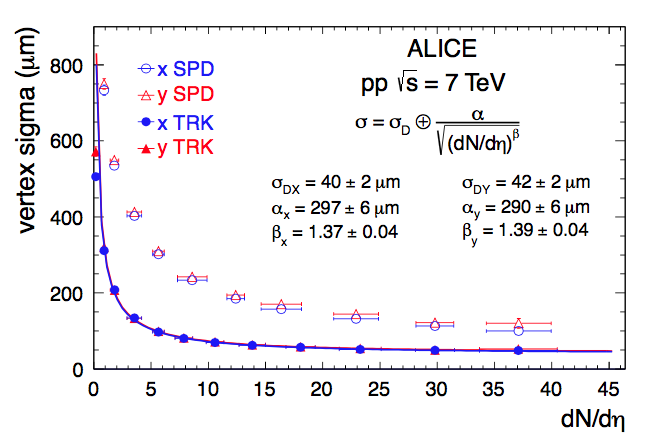
\includegraphics[width=.49\textwidth]{FigCap4/VtxReso.png}
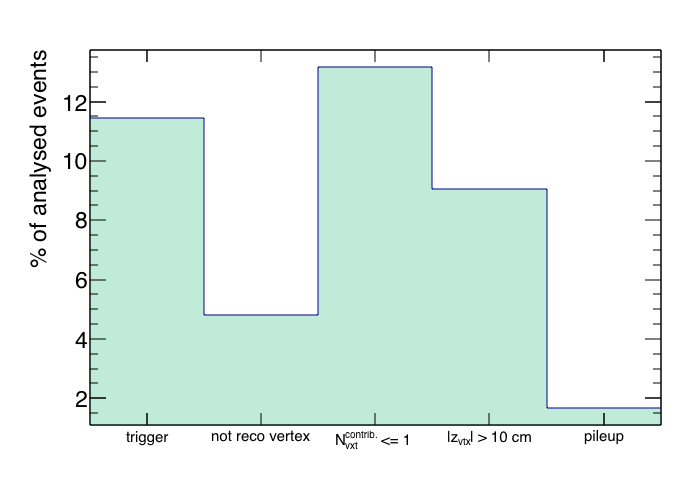
\includegraphics[width=.49\textwidth]{FigCap4/RejFracPass4.png}
\caption{Left: resolutions of $x$- and $y$- vertices reconstructed with SPD tracklets or global tracks as a function of the event multiplicity. Right: fractions of events rejected during vertex and physics selection.}
\label{fig:vxtReso}
\end{figure}



\section{$\Dsplus$ reconstruction and strategy}
\label{sec:DsRecoStrategy}
The $\Dsplus$ mesons can not be directly detected because of 
their mean proper decay length $c\tau = 150\pm 2$ $ \mu$m~\cite{Olive:2016xmw} 
that prevents them from reaching the detectors. Hence, the analysis is 
based on the reconstruction of the decay products.
$\Dsplus$ mesons and their antiparticles were 
 reconstructed in the decay channel $\Dstophipi$ 
 (and its charge conjugate) followed by $\PhitoKK$ 
 (Fig.~\ref{fig:DsDecayTopology}). The branching ratio (BR) of this decay channel 
 is 2.27 $\pm$ 0.08 \%~\cite{Olive:2016xmw}.
Other $\Dsplus$ decay channels can give rise to the same final products
 $\KKpi$, such as $\Dsplus\rightarrow {\rm  K^{*0} K^+}$ and 
 $\Dsplus\rightarrow f_o(980) \pi^+$ with BR  2.63 $\pm$ 0.13 \% and 
 1.16 $\pm$ 0.32 \%, respectively. It was verified that the selection efficiency for 
 these decay modes is strongly suppressed by the cuts applied 
 to select the signal candidates of $\DstophipitoKKpi$, that include 
 a selection on the mass of the intermediate resonant state. 
 Since the width of the $\phi$ peak is narrower than those of the 
 K$^{*0}$ and the $f_o(980)$, the decay channel through the 
 $\phi$ resonance, being the one that provides the best discrimination 
 between signal and background, was used in this analysis. 
 The $\Dsplus$ signal is extracted from 
 the invariant-mass\footnote{The invariant mass is defined as:\\ 
 \begin{align*} m^2 =& E^2 -\vec{p}^{\, 2} = (E_1 + E_2)^2 -(\vec{p_1} + \vec{p_2})^2 \\ m^2 =& m_1^2 +m_2^2 + 2(E_1E_2 -p_1p_2{\rm cos}\theta) \end{align*}} 
 distribution of the candidates, which are obtained by 
 combinatorial association of three reconstructed tracks with the correct 
 charge-sign combination. Hence, 
 the invariant-mass distribution will have a contribution from real 
 $\Dsplus$ decays ($\DstoKKpi$) and another 
 from background candidates. In order to improve the signal-to-background
ratio, specific cuts were applied on the decay topology, on
   the invariant mass of $\KK$ pair and on the particle identification, 
   as explained in the following sections. 
In particular, the selections based in the decay topology exploit the
fact that $\Dsplus$ meson mean proper decay length of $\sim 150\, \mu$m  
makes it possible to separate its decay vertex from the primary vertex
of the pp interaction. 
\begin{figure}[!t]
\centering
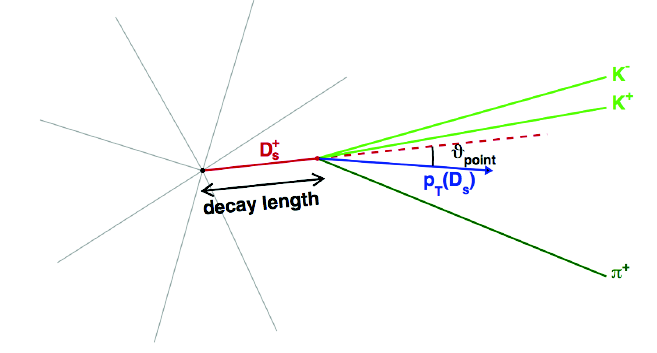
\includegraphics[width=12cm]{FigCap4/Ds.png}
\caption{Schematic view of the $\Dsplus\rightarrow \phi \pi^+ \rightarrow K^+K^-\pi^+$ decay.}
\label{fig:DsDecayTopology}
\end{figure}
Before the candidates go through specific selections on the decay
topology and particle identification, they have to pass single-track 
quality cuts. In the following, details of each selection step will
be illustrated. 



\section{Single-track selections}
\label{sec:singleTrCuts}
Reconstructed tracks were selected by requiring:
\begin{itemize}
\item successful fit with the Kalman filter in TPC and ITS (see Sec.~\ref{sec:tracking})
\item pseudo-rapidity $|\eta| < 0.8$
\item $\pt > 0.3~\GeV/c$
\item at least 70 (out of a maximum of 159)
associated space points in the TPC
\item ratio of crossed rows (total number of hit TPC pad rows, i.e. corrected 
for pad rows with missing signal) over findable clusters (pad rows which, 
based on the geometry of the track, are possible clusters) in the TPC larger than 0.8
\item $\chi^2/\mathrm{ndf} < 2$ for the track-momentum fit in the TPC (where ndf is the number of degrees of 
freedom involved in the tracking procedure)
\item at least two (out of six) hits in the ITS, out of which at least one 
in either of the two SPD layers
\end{itemize}
For tracks that satisfy the above selection criteria, the transverse momentum 
resolution is better than 1$\%$ at $\pt = 1\, \Gevc$ and about 2\% at $\pt = 10 \, \Gevc$. 
The resolution on the track impact parameter, which is the distance of closest 
approach of the track to the primary vertex, is better than 75 $\mu$m for 
$\pt >$ 1 $\Gevc$ for the projection on the bending plane ($r\phi$, normal to 
the beam direction) in pp collisions.
In order to have unbiased determination of the primary vertex, for each 
$\Dsplus$ candidate the interaction point was recalculated from the reconstructed 
tracks after excluding the candidate decay tracks.
\begin{figure}[!htbp]
\begin{center}
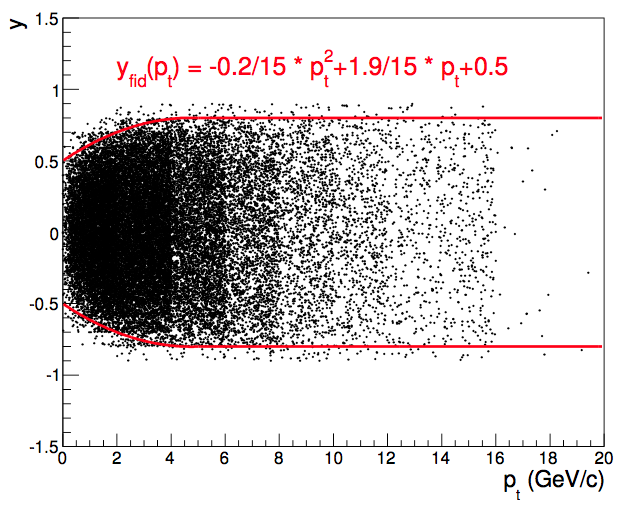
\includegraphics[width=.5\textwidth]{FigCap4/YvsPt.png}
\label{fig:singtrafter}
\caption{Rapidity versus $\pt$ distribution of the reconstructed $\Dsplus$ mesons. The fiducial acceptance region is defined by $|y| < y_{\rm fid}(\pt)$.}
\end{center}
\end{figure}

The single-track selection criteria reduce the $\Dsplus$-meson acceptance
in the rapidity-transverse momentum plane. The acceptance drops 
steeply to zero for $|y| > 0.5$ at low $\pt$ and for $|y| > 0.8$ 
at $\pt > 5~\Gevc$. A $\pt$-dependent fiducial acceptance region was therefore defined as 
$|y| < y_{\mathrm{fid}}(\pt)$, with $y_{\mathrm{fid}}(\pt)$ increasing 
from 0.5 to 0.8 in the transverse momentum range $0 < \pt < 5~\Gevc$ 
according to a second-order polynomial function, and $y_{\mathrm{fid}}=0.8$ 
for $\pt > 5~\Gevc$ (see Fig.~\ref{fig:singtrafter}):
\begin{equation}
\label{eq:yFid}
y_{\rm fid} (\pt) = -\frac{0.2}{15}\pt^2 + \frac{1.9}{15}\pt + 0.5.
\end{equation}

\section{Decay-chain and topology selection}
\label{sec:topolPP}
The $\Dspm$ candidates are built from combinatorial 
 association of three candidate tracks passing the selection criteria 
 described in Sec.~\ref{sec:singleTrCuts}, with the correct combination of charge 
 signs. In this way, a huge number of candidates (about 885M, corresponding to $\sim$3 candidates per event) 
 is created, most of them being combinatorial background. 
 Strict selections are therefore needed to increase
 the signal-to-background ratio and the statistical significance of the signal,
 by applying cuts on variables that have the potential to discriminate
 $\Dsplus$ signal (i.e. corresponding to real $\Dspm$ decays) 
 from background candidates. Candidates 
  are thus selected by applying geometrical cuts on the displaced decay vertex 
  topology, which are tuned as a function of the D-meson $\pt$.
The main feature of the $\Dsplus$-decay topology is the presence of three tracks displaced from 
the primary vertex and compatible with the hypothesis of being originated from 
a common point. 
The variable that allows one to evaluate the displacement of a track from the interaction point is its 
impact parameter, whose resolution is mostly determined by the hits in the 
two SPD inner layers of the Inner Tracking System. \\
The request of a minimum $\pt = 0.3$ $\Gevc$ of the daughter tracks contributes to 
the background rejection exploiting the harder  $\pt$ distribution of
the $\Ds$ decay products with respect to the background tracks. 
The other selections are applied by exploiting the secondary vertex
which is reconstructed from the three tracks that compose the $\Ds$
candidate. The topological cuts used for $\Dspm$ signal selection
 are explained in detail below. Fig.~\ref{fig:var1},~\ref{fig:var2} and~\ref{fig:var3} complement
 the description, showing distributions of some of the below listed variables
 for prompt signal (in red) and background (in blue) candidates, in the interval $2 < \pt < 16 \, \Gevc$, 
 extracted from Monte Carlo production (PYTHIA~\cite{Sjostrand:2006za}) and data, respectively.
 The distributions in data are obtained from candidate triplets with very loose
 selections on the topological variables, thus the contribution from the signal is negligible.
 The beauty feed-down component (also obtained from MC) is shown
 in green curve for those variables whose distributions for prompt signal
 from charm decays and for feed-down signal from beauty decays are different.
 
\begin{itemize}
\item \textbf{Decay length $D_{len}$}, defined as the distance between
 primary and secondary vertex. $\Dspm$ decay vertices are displaced by
  a few hundred $\mu$m from the interaction vertex ($c\tau \approx 150\, \mu$m). Since real $\Dspm$ 
  decay vertices have, on average, larger values of decay length than the
   background, as it can be seen in Fig.~\ref{fig:var1} (left), 
   this allows one to discriminate signal from background. 
   Likely cut values are $D_{len} > 300-400\, \mu $m. 
   To be noted that $\Ds$ mesons coming from weak decays of beauty hadrons have larger $D_{len}$
   with respect to prompt $\Ds$ from charm decay, due to more displaced decay vertices.
\item \textbf{Normalized decay length NDL$_{\rm xy}$}, defined as the decay length 
in the transverse plane ($xy$) divided by its uncertainty (Fig.~\ref{fig:var1} right).
Typical values of cuts on this variable are around 2.
\item \textbf{Cos$\theta_{point}$}, where $\theta_{point}$ is the angle
 between the momentum of the reconstructed $\Dspm$ meson and the 
 $\Dspm$ flight line (line connecting primary and secondary vertex, see
  left panel in Fig.~\ref{fig:var2}). The pointing angle is expected to be small for signal 
  candidates, resulting in a distribution of cos$\theta_{point}$ peaking at 1 for 
  signal and being broader for background candidates. Hence, cuts like 
  cos$\theta_{point} >$ 0.93 or tighter were usually applied to reject background.
\begin{figure}[!t]
\centering
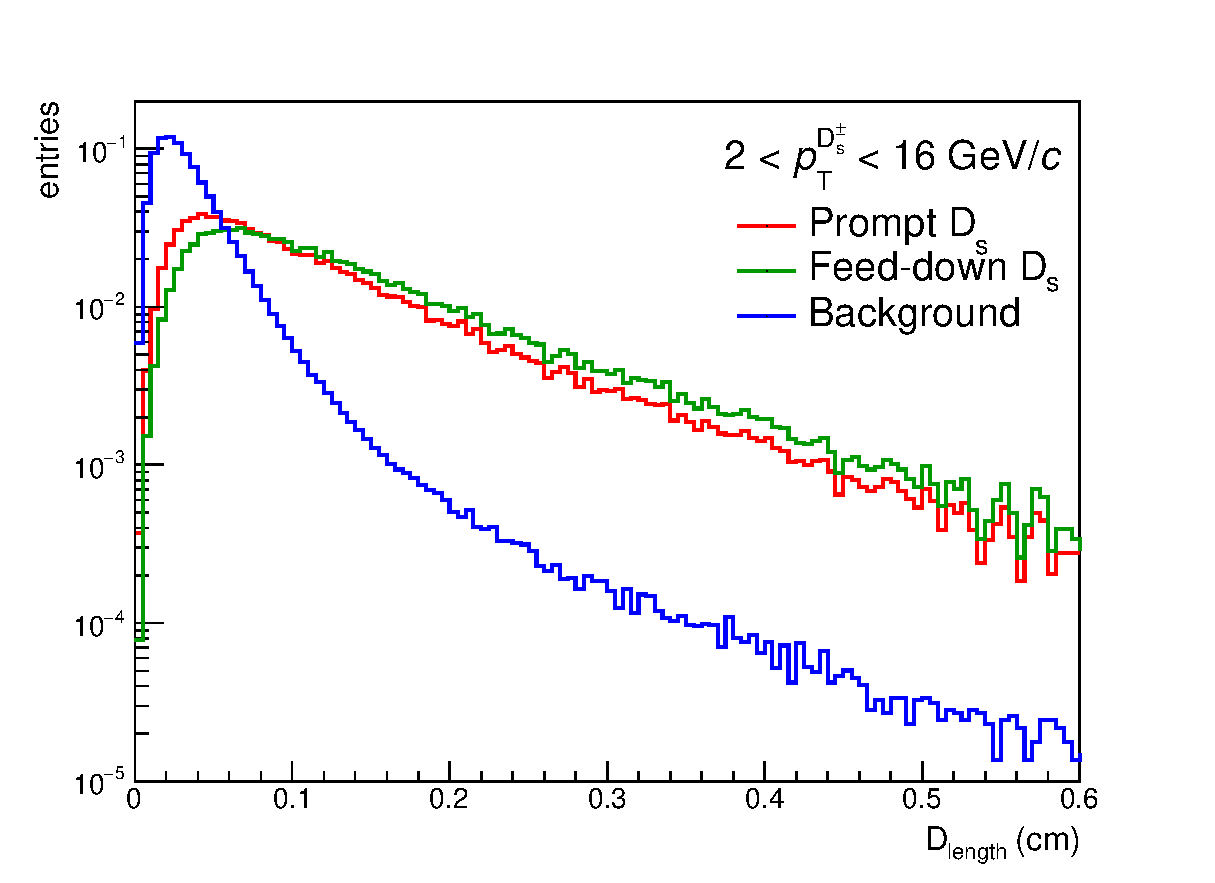
\includegraphics[width=6.5cm]{FigCap4/DL.eps}
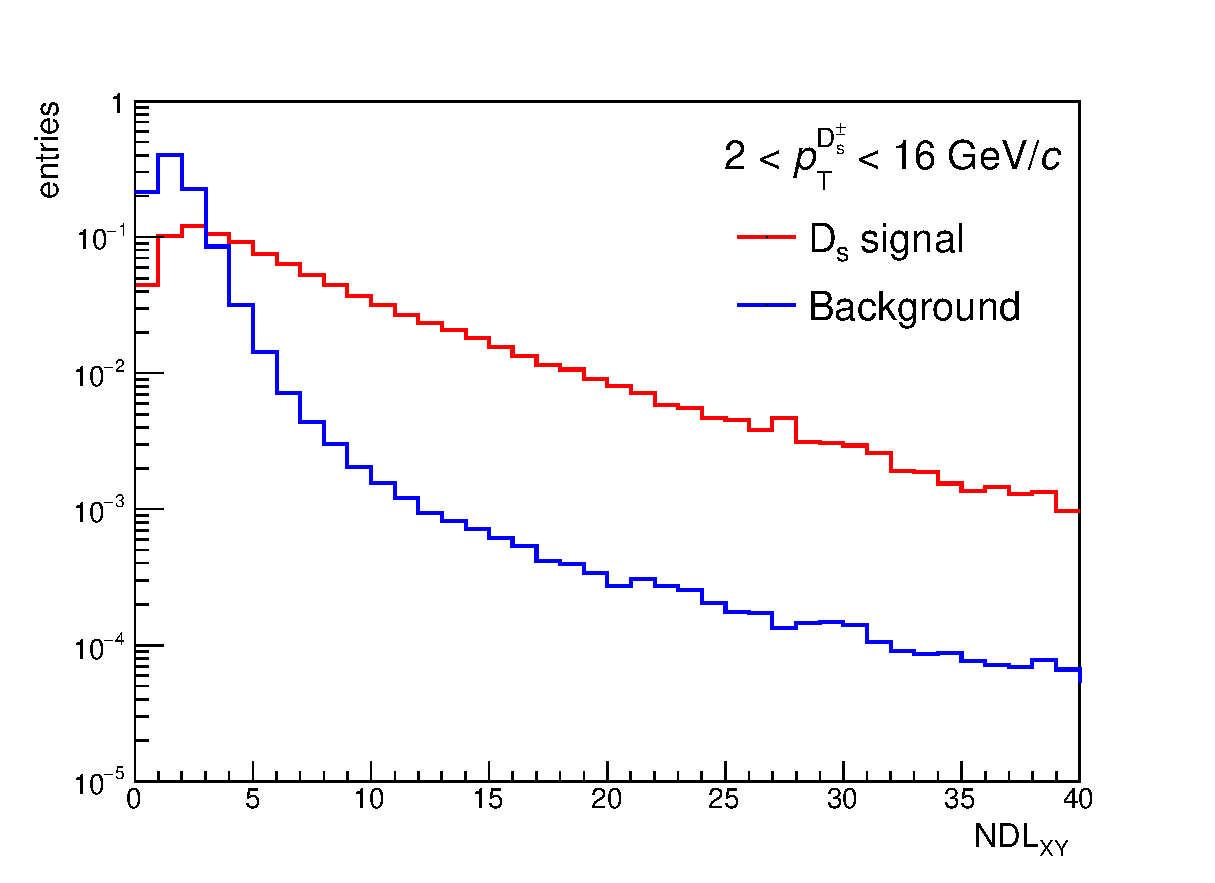
\includegraphics[width=6.5cm]{FigCap4/NDLxy.eps}
\caption{Left: distributions of decay length for prompt (red), feed-down (green) signal and background (blue) $\Ds$ candidates. Right: distributions of normalised decay length in the transverse plane signal (red) and background (blue) $\Ds$ candidates.}
\label{fig:var1}
\end{figure}
\begin{figure}[!h]
\centering
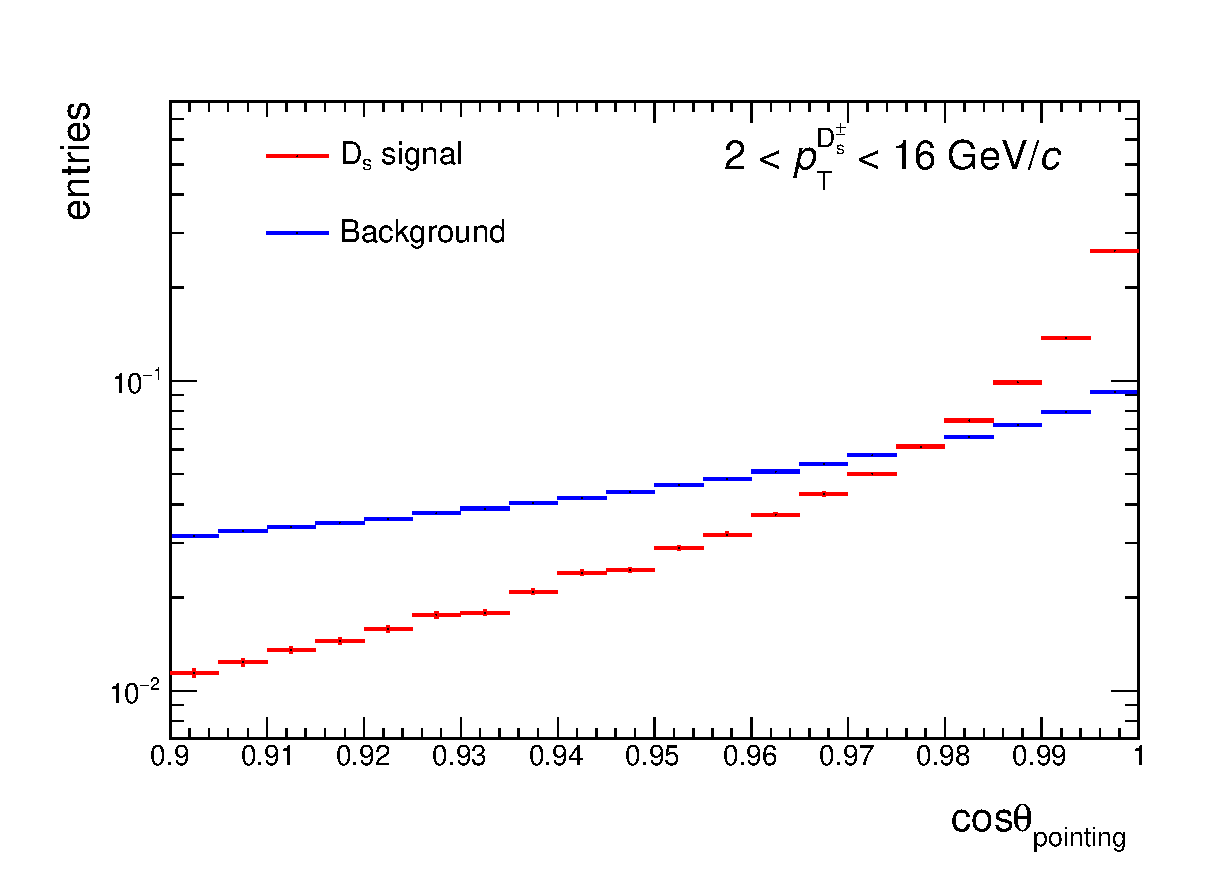
\includegraphics[width=6.5cm]{FigCap4/cosP.eps}
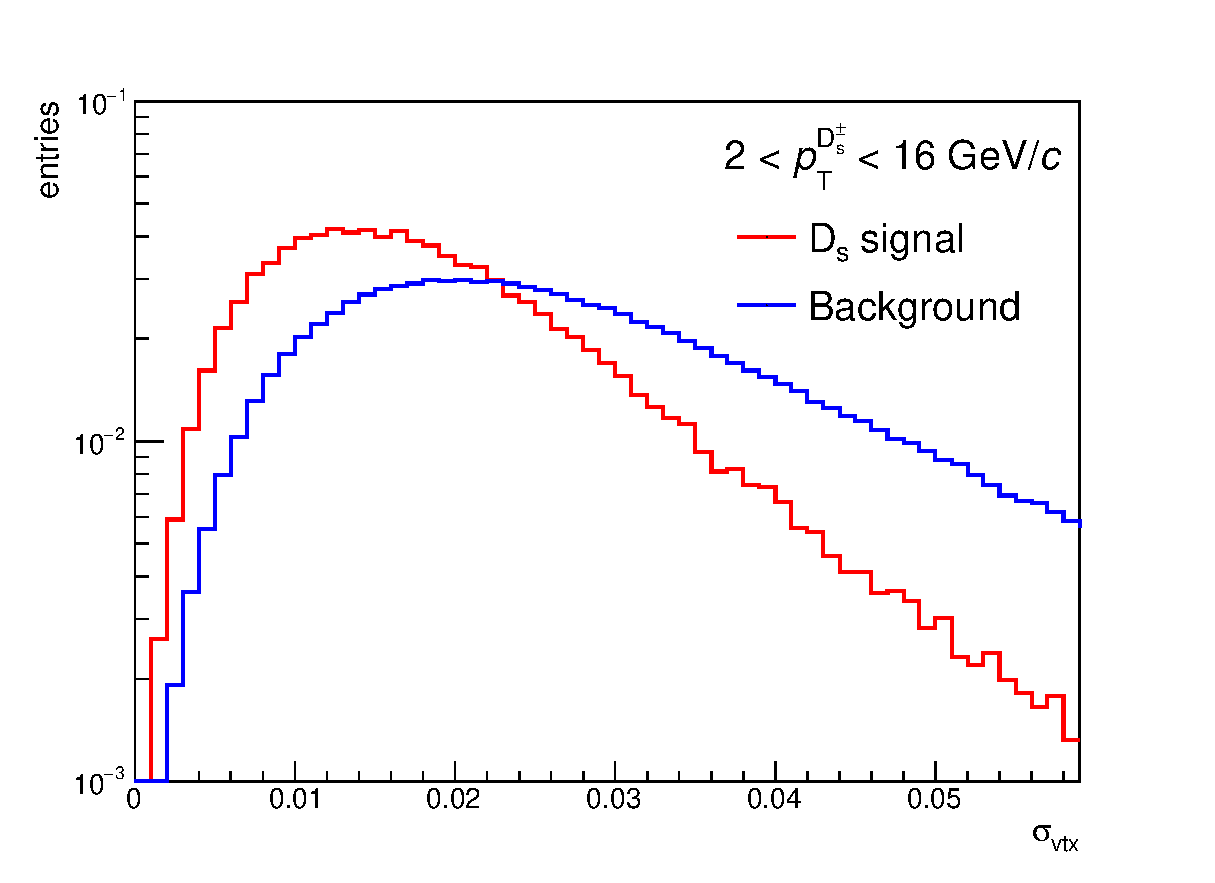
\includegraphics[width=6.5cm]{FigCap4/sigVert.eps}
\caption{Distributions of cos$\theta_{point}$ (left) and track dispersion around secondary vertex $\sigma_{vtx}$ (right) for signal (red) and background (blue) $\Ds$ candidates.}
\label{fig:var2}
\end{figure}
\begin{figure}[!h]
\centering
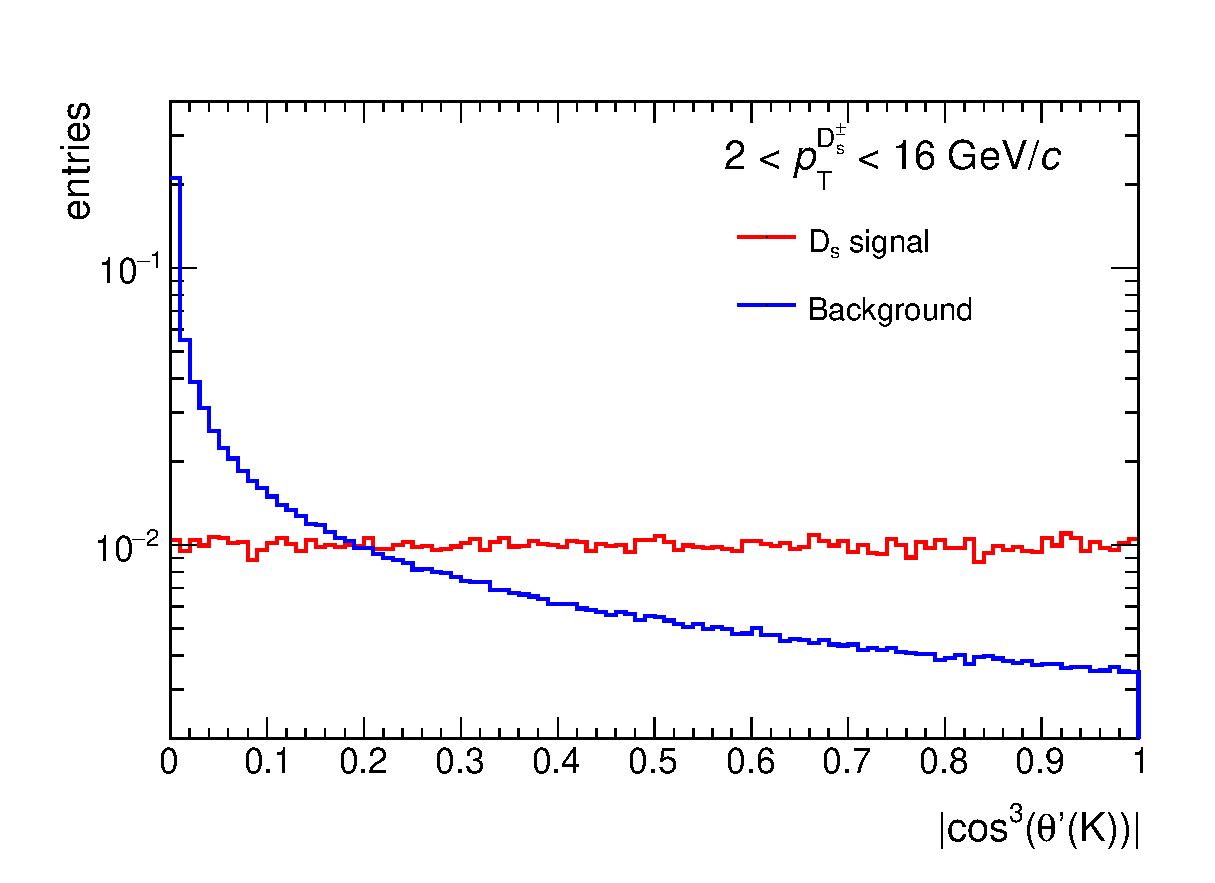
\includegraphics[width=6.5cm]{FigCap4/CosPiKPhi3.eps}
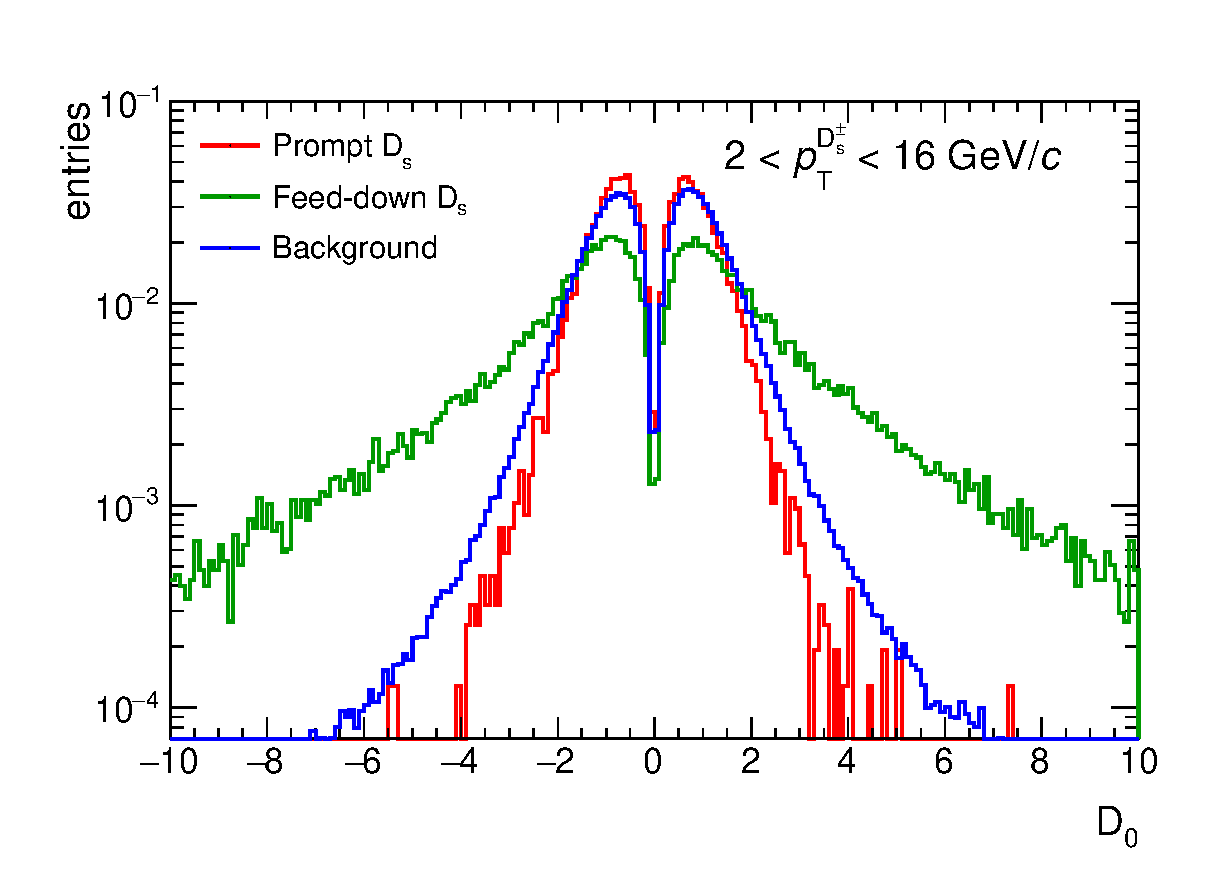
\includegraphics[width=6.5cm]{FigCap4/normIP.eps}
\caption{Left: distributions of $|{\rm cos}^3(\theta'(K))|$ for signal (red) and background (blue) $\Ds$ candidates. Right: distributions of maximum normalised single-track impact parameter among the three $\Ds$ daughters, in the transverse plane, for prompt (red), feed-down (green) signal and background (blue) $\Ds$ candidates.}
\label{fig:var3}
\end{figure}

\item \textbf{Track dispersion $\sigma_{vtx}$} around the decay vertex, defined as:
\[
\sigma_{vtx}=\sqrt{d^2_1+d^2_2+d^2_3}
\]
where $d_i$ is the distance of minimal approach between the decay 
track \textit{i} and the decay vertex. All tracks should originate from 
the secondary vertex, and $\sigma_{vtx}$ should be $\sim$ 0; in 
real cases, as a consequence of the tracking and vertex finding resolution, 
the $\sigma_{vtx}$ has non-zero values and an upper cut is needed 
to exclude vertices made of random combination of tracks. Typical cut
 values on the track dispersion were between 0.02 $< \sigma_{vtx}<$ 0.05 cm 
 (see Fig.~\ref{fig:var2} right).
\item \textbf{$\theta^*(\pi)$ angle}, it is the angle between the pion 
in the KK$\pi$ rest frame and the KK$\pi$ flight line. Cuts were applied
 on the distribution of the cos$\theta^*(\pi)$, with typical values 
 between 0.95 $<{\rm cos}\theta^*(\pi)  <$ 1.0.
\item \textbf{$\theta'$(K) angle}, it is defined as the angle between
 one of the kaons and the pion in the KK rest frame. Cuts were 
 applied on the distribution of the $|{\rm cos}^3(\theta'(K))|$ (Fig.~\ref{fig:var3}, left), with typical 
 values between 0.0 $<|{\rm cos}^3(\theta'(K))| <$ 0.05.
 The selections on $\theta^*(\pi)$ and $\theta'$(K) angles have already 
been used in various experiments which measured $\Dsplus$ production 
like ZEUS \cite{Chekanov:2005mm} and ATLAS \cite{ATLAS:2011fea} as well as 
in previous ALICE analyses~\cite{ALICE:2011aa,Abelev:2012tca,Adam:2016ich,Adam:2015jda}
 and are based on kinematical 
considerations on the decay chain with a $\phi$ in the intermediate state.
\item \textbf{Single-track normalised impact parameter residual $D_{0}$} : it is defined 
as the difference between the expected 
impact parameter value $d^{exp}_{0,r,\phi} \approx D_{len}^{xy} \cdot {\rm sin}(\theta_{xy})$
 ($D_{len}^{xy}$ is the decay length on $xy$ plane and $\theta_{xy}$ is the angle 
between the reconstructed D-meson momentum and the $i$-th daughter track on $xy$ plane) 
and the reconstructed one $d^{reco}_{0,r,\phi}$ for the $i$-th daughter
track. The difference $d^{reco}_{0}-d^{exp}_{0}$ is normalised by its uncertainty
calculated as the sum in quadrature of the uncertainties on $d^{reco}_{0}$ and $d^{exp}_{0}$.
In Fig.~\ref{fig:var3} (right) the distributions of the $D_{0} = max[d^{reco}_{0}-d^{exp}_{0}/\sigma]$ among 
the three daughter tracks of $\Ds$ candidates are shown, in different colours for
background and signal candidates, distinguished between prompt and beauty 
feed-down components. Since the distributions of $D_{0}$ 
are quite different for prompt and feed-down D mesons, 
a selection based on this variable can reduce the feed-down D-meson contribution with respect to 
that of prompt D mesons. In this analysis selections on the $D_{0} \sim 2$
were applied.
\end{itemize}

  New topological variables were introduced with respect to the 
  previous analysis of this sample. They are the projections of the cosine of 
the Pointing angle and of the (normalised) decay length in the $xy$ plane 
 and the single-track normalised impact parameter residual.
The projections of the variables in the $xy$ plane are justified by 
the better resolution of the impact parameter resolution with respect to $z$-direction.\\


A further selection which allowed to reduce the background is the requirement that the
 \textbf{invariant mass of the reconstructed $K^+K^-$ pair} is compatible 
 with the $\phi$-meson mass. This is not a topological 
 cut (i.e. a cut exploiting the displacement of the decay vertex), 
 but a selection on the decay chain. It is required that at least 
 one of the two pairs of tracks with opposite charge has an invariant
  mass compatible with the $\phi$ mass when the kaon mass is assigned to
  the two tracks. The selection is done on 
  the absolute value of the difference between the $\phi$ 
   invariant mass from PDG ($\sim 1.019\, \Gevc$) and the reconstructed one:
\[
\Delta M = |M^{inv}_{rec}-M_{\phi}|.
\]
Typical values for cuts on $\Delta M$ are between 3 $<\Delta M<$ 15 MeV$/c^2$,
thus always preserving more than 85\% of the signal.

\section{Particle identification}
\label{Sec:PID}
The Particle IDentification (PID) selection is based on the specific energy loss 
d$E$/d$x$ in the TPC and the time-of-flight from the interaction vertex to the 
TOF detector. This is used in the D-meson analysis to reduce the background, 
and it is essential for $\Dsplus$ studies because of the low values of signal-over-background
 ratios (S/B).
A track is  considered compatible with a certain particle species 
($\pi$, K or p) if the measured signal has a difference 
within $n\sigma$ from the expected one for the corresponding mass hypothesis:
\[
|S_{meas}-S^{\pi,k,p}_{expected}| < n^{\pi,k,p}\sigma ,
\]
where $\sigma$ is the resolution on the energy-loss or time-of-flight signals for each species
and $S^{\pi,k,p}_{expected}$ is the expected signal in TPC or TOF
calculated respectively with Bethe-Bloch or time-of-flight equations for a given mass hypothesis (see Sec.~\ref{sec:TPC} and~\ref{sec:TOF}).
Candidate triplets were required to have two tracks compatible with 
the kaon hypothesis and one with the pion hypothesis. In addition, 
since the decay particle with opposite charge sign with respect to the $\Dsplus$
mother particle in the $\DstoKKpi$ chain has to be a kaon, 
a triplet was rejected if the opposite-sign track was not compatible 
with the kaon hypothesis. 
The criterion used to classify tracks on the basis of their PID
information in TPC and TOF detectors is 
illustrated in Fig.~\ref{fig:strongPID}, where $n\sigma^{\rm max,TPC} = 1$ for
$0.6 < \pt < 0.8 \, \Gevc$ and 2 elsewhere and $n\sigma^{\rm max,TOF} = 3$ at all $\pt$.  
A response value of -1, 0 or 1 (green values in Fig.~\ref{fig:strongPID}) 
is assigned to the PID signal in each
detector. For both detectors, a final response value of -1 is assigned   
if the PID signal of the track is different from the expected one
by more than 3$\sigma$. In cases where the TPC or TOF information is not
available, a response value of 0 is assigned
to the detector. This holds in particular for tracks at low momentum that may not reach the TOF.  
To combine PID information in the two detectors,
the response values in TPC and TOF 
are summed together and the track is considered
compatible with a species hypothesis if the combined response value is 1 or 2. This
PID selection preserves $\sim$85-90\% of the signal depending on the $\pt$.

 
\begin{figure}[!h]
\centering
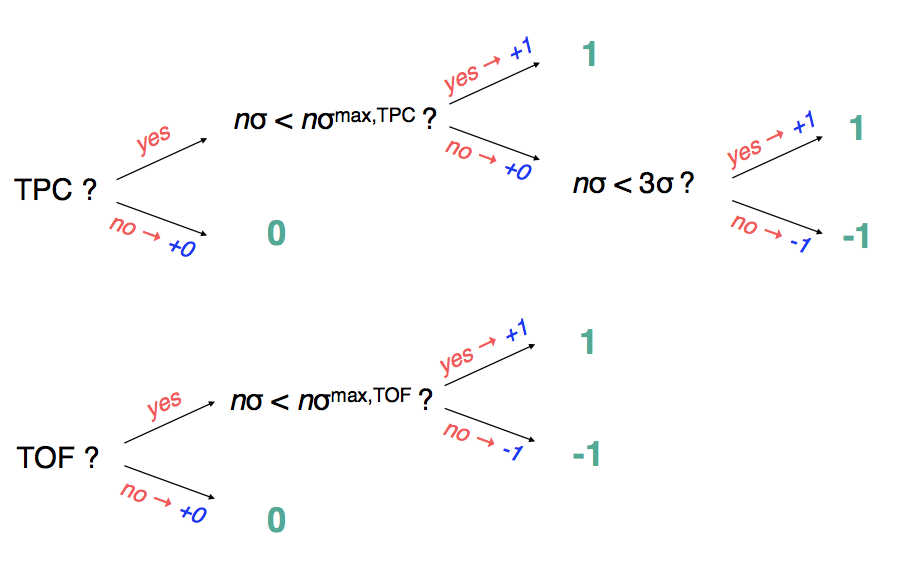
\includegraphics[width=11cm]{FigCap4/strongPID.png}
\caption{PID selection criteria in TPC and TOF for a specific mass hypothesis.}
\label{fig:strongPID}
\end{figure}


\section{Invariant mass spectra, cut optimization and signal extraction}
\label{sec:invMassPlotsPP}
For each candidate, two values of invariant mass can be computed, 
corresponding to the two possible assignments of the kaon and the 
pion mass to the two same-sign tracks. Considering the $\Dsplus$
 decay, the charge configuration of the tracks (+, -, +) can be interpreted
  both as to ($K^+,K^-,\pi^+$) and ($\pi^+,K^-,K^+$) mass assignments. 
     Candidates were rejected if none of the two pairs of opposite-charged 
   tracks had an invariant mass compatible with the PDG world average for the $\phi$ mass.
Signal candidates with 
  wrong mass assignment to the same-sign tracks would give rise to 
  a contribution to the invariant mass distributions that could introduce
   a bias in the extraction of the raw yield of $\Dsplus$ mesons.
   It was verified, both in data and in simulations, that the particle identification and the requirement 
   on the invariant mass of the two tracks identified as kaons to be compatible with the
$\phi$ PDG mass reduce the bias contribution to a negligible level.
$\Dsplus$ candidates that pass all the selections are 
used to fill invariant mass histograms in different intervals of candidate $\pt$.
The histograms are fitted by a function consisting of a sum of 
a Gaussian and an exponential function to describe the signal peak and 
the background shape respectively:
\begin{equation}
f(x)= Ae^{-B\cdot x}+Ce^{-\frac{(x-\mu)^2}{2\sigma^2}}.
\end{equation}
The selection criteria used in the analysis as  ``central cuts'' were tuned to 
preserve high selection efficiency and high statistical 
 significance for the D meson signal, defined as:
\[
Signif = \frac{\rm S}{\sqrt{\rm S+B}},
\]
where S and B are the extracted signal and background obtained 
from the fit procedure integrated within 3$\sigma$ 
around the peak of the Gaussian ($\sigma$ being the
Gaussian width of the peak from the fit). The statistical significance is related to the 
relative statistical uncertainty on the extracted signal, so higher 
significance means lower statistical uncertainty on the raw yield. 
A third variable which is considered in the cut optimisation procedure
 is the signal-over-background ratio S/B. It was also
required that the position and the width 
  of the Gaussian peak were compatible with the values
   obtained in simulated events, with the same selection strategy.
The selection values depend on the $\pt$ of the $\Ds$-meson candidate, since
the number of background candidates depends on $\pt$ as well.
At low momentum, where the contribution from the combinatorial
background is dominant, tighter selections are needed but, due to less displaced 
vertices with respect to the higher $\pt$ candidates which are more boosted, too strong selections
on the decay topology (e.g. decay length) are not allowed.
The cuts used in the analysis are detailed in Table~\ref{tab:cutsDs}.
The number of $\Ds$ candidates per event, after all the selections described above, is about 0.02.
\begin{table}[tbh!]
\centering
\begin{tabular}{|l|c|c|c|c|} 
\hline 
 $\Ds$ meson& \multicolumn{4}{c|}{pt interval (GeV/$c$)}\\
\hline
 & 2--4  & 4--6 & 6--8 & 8--12\\
\hline
Decay length ($\mum$)        & $>$300 & $>$350 & $>$350 & $>$400\\
Decay length XY ($\mum$)     & $>$0 & $>$200 & $>$200 & $>$200\\
Norm Decay length XY          & $>$2.0& $>$0.0 & $>$2.0 & $>$2.0\\
Cosine pointing              & $>$0.94 & $>$0.95 & $>$0.94 & $>$0.94\\
$\sigma_{vtx}$  (cm)          & $<$0.02 & $<$0.03 & $<$0.03 & $<$0.06\\
$\Delta M$ (MeV/$c^{2}$) & $<$8.0 & $<$10.0 & $<$4.5 & $<$9.0\\
$\cos \theta^*(\pi)$    & $<$1.0 & $<$1.0 & $<$1.0 & $<$0.95\\
$|\cos^3 \theta^\prime({\rm K})|$        & $>$0.10 & $>$0.05 & $>$0.05 & $>$0.05\\
Norm. IP residual Kaon  & $<$2.5 & $<$2.0 & $<$2.0 & $<$2.0 \\
Norm. IP residual Pion  & $<$2.5 & $<$2.0 & $<$2.0 & $<$2.0 \\[1ex]
\hline
\end{tabular}
\caption{Selections used for the $\Dspm$ meson in the four transverse momentum intervals considered.} 
\label{tab:cutsDs}
\end{table}
In Fig.~\ref{fig:invmassDs} the invariant mass distributions 
of $\Dspm$ mesons in four $\pt$ intervals from 2 to 12 $\Gevc$ are shown 
and the values of S/B, statistical significance and extracted yields 
with their statistical uncertainties are reported in Table~\ref{tab:signalDs}.
\begin{figure}[!htb]
\begin{center}
 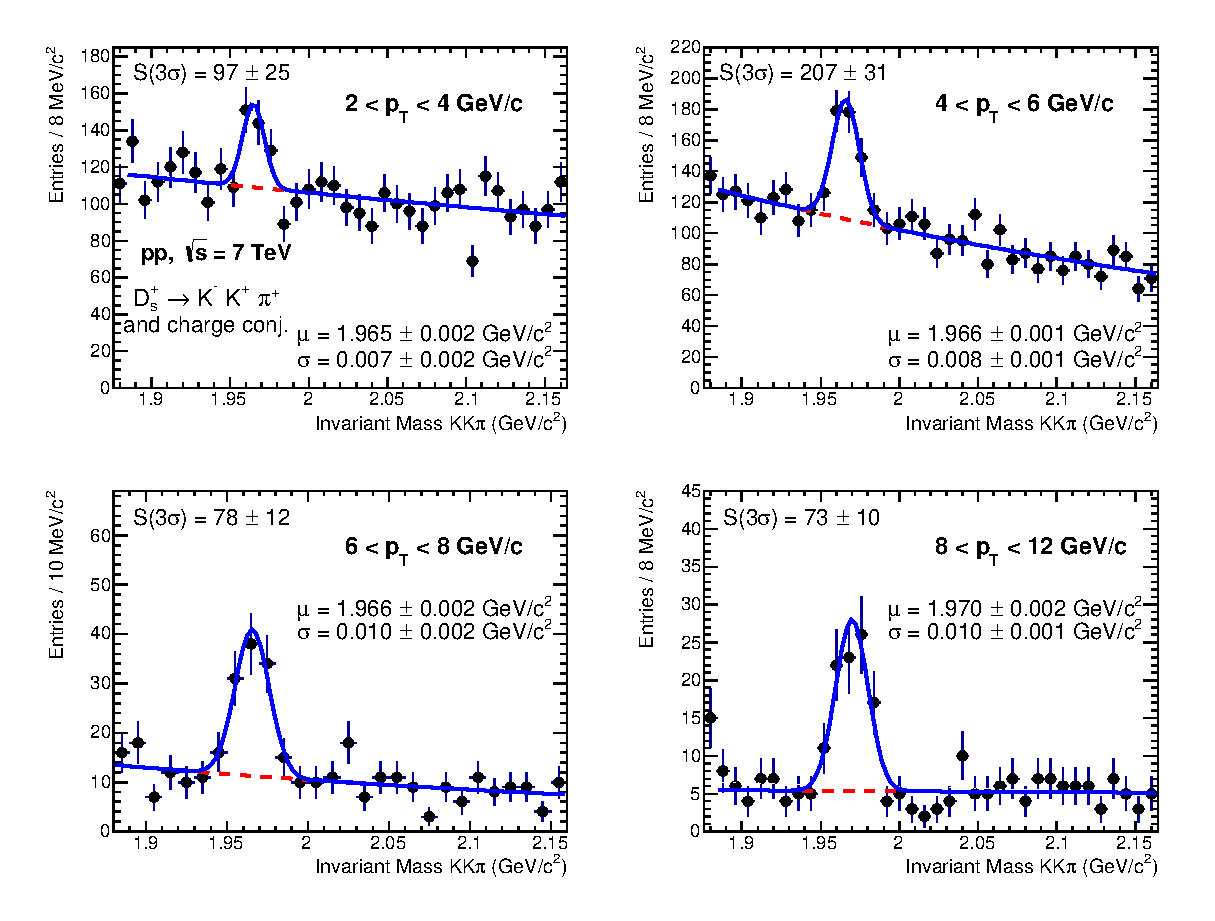
\includegraphics[width=.99\textwidth]{FigCap4/DsMassHistos_ppPass4.eps}
\caption{Invariant mass distributions of $\Dsplus$ candidates and charge
conjugates in the four considered $\pt$ intervals.}             
\label{fig:invmassDs}
\end{center}
\end{figure}
\begin{table}[tbh!]
\centering
\begin{tabular}{|l|c|c|c|} 
\hline
 $\pt$ ($\Gevc$) & S/B  & Signif. & S(3$\sigma$)\\
\hline
2-4   & 0.18 & 3.8 & 97 $\pm$  25\\
4-6    & 0.30 & 6.9 & 207 $\pm$ 31\\
6-8    & 1.10 & 6.4 & 78 $\pm$ 12\\
8-12  & 1.78 & 6.8 & 73 $\pm$ 10\\
\hline
\end{tabular}
\caption{S/B, statistical significance and yield for $\Dspm$ signal peak in the four transverse momentum intervals considered.} 
\label{tab:signalDs}
\end{table}

An indication of the improved resolution provided by the new 
reconstruction of the sample is shown in the left panel of Fig.~\ref{fig:sigma4vs2}, where the 
Gaussian sigmas of the simulated signal peak for the current and old
reconstruction are compared. In the right
panel of the same figure, the Gaussian widths of $\Ds$ peak are shown 
as a function of $\pt$ for the current reconstruction in data (solid points)
and in MC (dashed) and the values agree within uncertainties. 
\begin{figure}[!hb]
\begin{center}
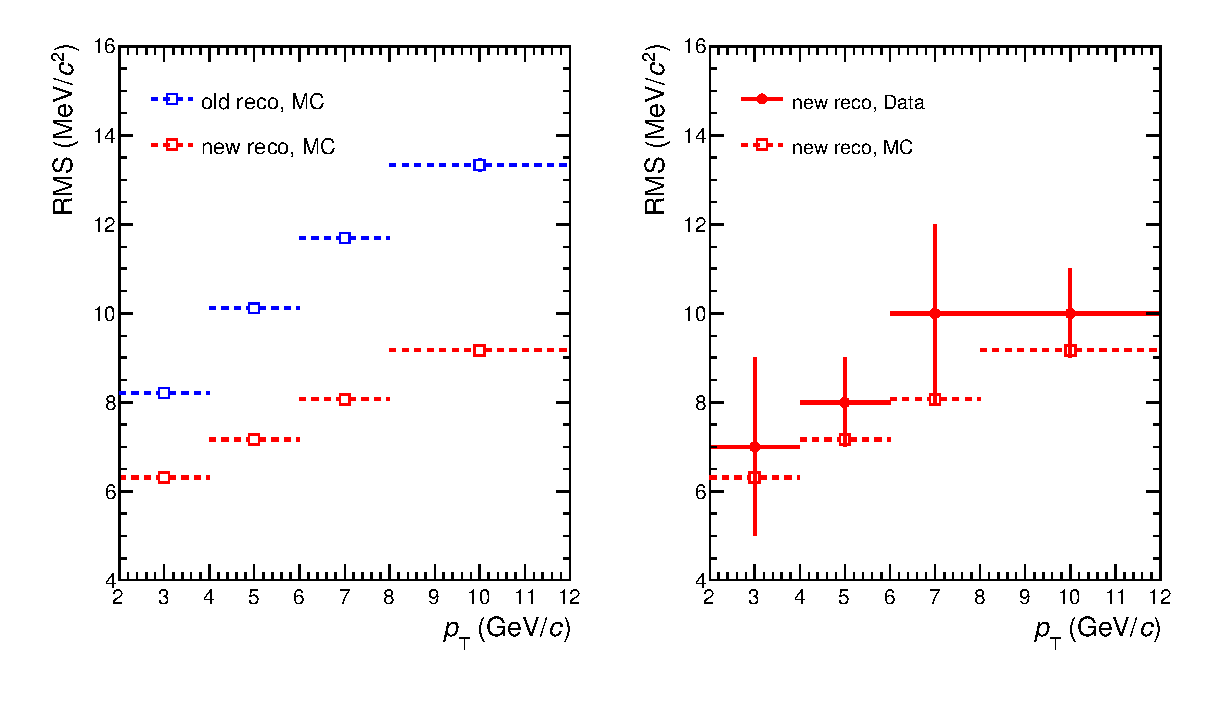
\includegraphics[width=.9\textwidth]{FigCap4/Resolutions_pass2_pass4.eps}
\caption{Left: MC Gaussian widths of $\Ds$ peak as a function of $\pt$, for current (red) and previous (blue) reconstruction. Right: Gaussian widths of $\Ds$ peak as a function of $\pt$ for current reconstruction in data (solid) and MC (dashed). }
\label{fig:sigma4vs2}
\end{center}
\end{figure}

\begin{figure}[!hb]
\begin{center}
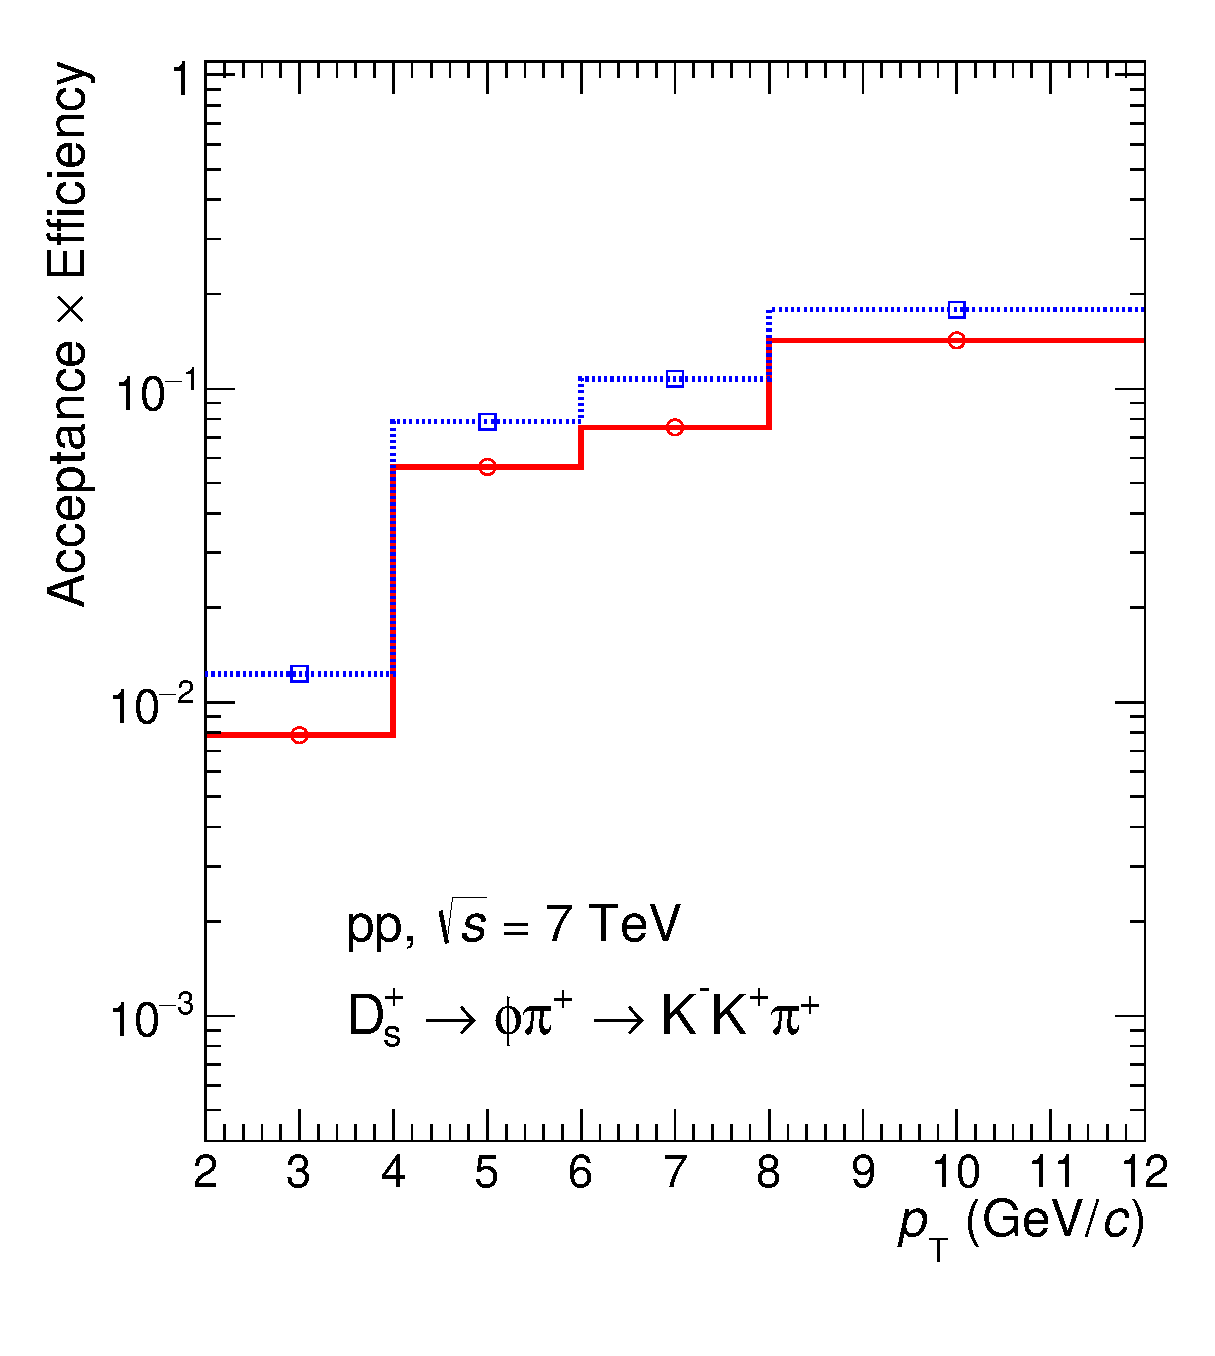
\includegraphics[width=.52\textwidth]{FigCap4/AccEff_Ds_Pass4.eps}
\caption{Acceptance-times-efficiency of prompt and feed-down $\Ds$ mesons as a function of $\Ds$ $\pt$.}
\label{fig:sigma4vs2}
\end{center}
\end{figure}

\section{Corrections}
\label{sec:corrPP}
The $\Dspm$ raw yields (sum of particle and anti-particle) extracted from the fits to the invariant-mass distributions
were corrected to obtain the $\pt$-differential production cross sections of prompt
 $\Dsplus$ mesons. The production cross section was calculated as:
\begin{equation}
  \label{eq:dsdptPP}
  \left.\frac{{\rm d} \sigma^{\rm D^{+}_{\rm s}}}{{\rm d}\pt}\right|_{|y|<0.5}=
  \frac{1}{ \Delta \pt}\frac{1}{{\rm BR} \cdot L_{\rm int}}\frac{\left.f_{\rm prompt}(\pt)\cdot \frac{1}{2} N^{\rm D^\pm_{\rm s}~raw}(\pt)\right|_{|y|<y_{\rm fid}}}{ C_{\Delta y} \,({\rm Acc}\times\epsilon)_{\rm prompt}(\pt)}\,,
\end{equation}
where $N^{\rm D^\pm_{\rm s}~raw}(\pt)$ is the value of the raw yield 
(sum of particles and antiparticles),
 which needs to be corrected for the B-meson decay feed-down contribution 
(i.e.\ multiplied by the prompt fraction $f_{\rm{prompt}}$), divided by the 
acceptance-times-efficiency of prompt $\Ds$ mesons 
$(\rm Acc \times \epsilon)_{\rm{prompt}}$, and divided by a factor of two to 
obtain the charge (particle and antiparticle) averaged yields.
The corrected yields were further divided by the decay channel branching ratio (BR), 
the $\pt$ interval width ($\Delta \pt$), the rapidity coverage 
($C_{\Delta y} = 2 y_{\rm fid}$) and the integrated luminosity $L_{\rm int}$.
The rapidity acceptance correction factor $C_{\Delta y}$ was computed with the PYTHIA 6.4.21 event generator
with Perugia-0 tune as the ratio between the generated D-meson yield in $\Delta y = 2y_{\rm fid}$, 
(with $y_{\rm fid}$ varying from 0.5 at low $\pt$ to 0.8 at high $\pt$) 
and that in $|y| < 0.5$. It was checked that calculations of the $C_{\Delta y}$ correction 
factor based on FONLL pQCD calculations or on the assumption of uniform D-meson
rapidity distribution in $|y| < y_{\rm fid}$ would give the same result, 
because both in PYTHIA and in FONLL the D-meson yield is uniform within 1\% in the range $|y| < 0.8$.
The integrated luminosity ($L_{\rm int} = (6.0 \pm 0.2) {\rm nb}^{-1}$) was computed as $L_{\rm int} = N_{ev}/\sigma_{pp,MB}$,
where $N_{ev}$ is the number of analysed events and 
$\sigma_{pp,MB} = 62.2$ mb~\cite{Abelev:2012sea}
is the cross-section for the minimum-bias trigger condition, derived from
a van der Meer scan measurement~\cite{vanderMeer:296752}.

\subsection{Reconstruction and selection efficiency}
\label{sec:Effpp}
The acceptance-times-efficiency correction factor, 
$(\rm Acc \times \epsilon)$, was determined for the $\Ds$-meson
hadronic decay considered in this analysis using Monte Carlo simulations 
of pp collisions generated with the PYTHIA 6.4.21 event generator~\cite{Sjostrand:2006za} with the 
Perugia-0 tune~\cite{Skands:2010ak} and particle transport through the apparatus 
using GEANT3~\cite{Brun:1994aa}.
The luminous region distribution and the conditions (active channels, gain, 
noise level and alignment) of all the ALICE detectors were included in the 
simulations, considering also their evolution over time during the 2010 LHC 
data taking period.
In the production, only events containing a $c\bar{c}$ or a $b\bar{b}$ pair 
were transported through the apparatus and reconstructed, and
D mesons were forced to decay hadronically via the decay channels relevant to
the specific analyses.
The efficiency was extracted separately for prompt and feed-down D-mesons and 
is shown in Fig.~\ref{fig:sigma4vs2}, for the selection criteria
reported in Tab.~\ref{tab:signalDs}.
D mesons from beauty-hadron decays have higher efficiency than
the prompt ones in all the $\pt$ intervals, due to the larger average displacement of their 
decay vertices from interaction point.
The efficiency increases with $\pt$ because at higher $\pt$ 
the background is less dominant and looser selections are allowed. 
In general, with the chosen topological selections, efficiencies in this analysis
are on average 15\% lower than those used in the previously published analysis~\cite{Abelev:2012tca}. 
The present analysis uses more powerful selection variables 
(projections on $xy$ plane and impact parameter residual) that
enhance the signal-over-background ratio for $\Ds$ meson by a factor 
from 2 to 5 depending on the $\pt$ interval, with a slight reduction
of the global efficiency. Large signal-over-background ratios are indeed essential 
to assure a good stability of the extracted yield.

\subsection{Beauty feed-down subtraction}
\label{sec:ppFprompt}
The $f_{\rm prompt}$ fraction was calculated using the beauty production cross sections from  
FONLL calculations~\cite{Cacciari:1998it, Cacciari:2001td}, the 
$\mathrm{B} \rightarrow \mathrm{D} + X$ decay kinematics from the EvtGen package~\cite{Lange:2001uf} 
and the efficiencies for feed-down D mesons reported in 
Fig.~\ref{fig:sigma4vs2}:
\begin{equation}
\label{eq:fpr}
\begin{split}
f_{\mathrm{prompt}} = \, & 1- \frac{N^{\text{D~feed-down}}_{\mathrm{raw}}}{N^{\mathrm{D}}_{\mathrm{raw}}}=\\
& 1- \left (\frac{\rm d^2 \sigma}{\mathrm d\pt \mathrm d y} \right)^{\rm FONLL}_{\text{feed-down}} \cdot \frac{(\mathrm{Acc} \times \epsilon)_\text{feed-down} \cdot C_{\Delta y} \Delta \pt \cdot \mathrm{BR} \cdot L_{\rm int}}{N^{\rm D +\overline{D},raw}/2}\,,
\end{split}
\end{equation}
where the $\pt$ dependence of $f_{\rm prompt}$, $N^{\rm D +\overline{D},raw}$ and
$(\mathrm{Acc} \times \epsilon)_\text{feed-down}$ is omitted for brevity.
The values of $f_{\rm prompt}$ of $\Ds$ meson vary between 0.89 and 0.92 as a function
of $\pt$ and are shown in Fig.~\ref{fig:fpromptAndMT} (left). 
The prompt fraction decreases with $\pt$
due to topological cuts, such as the decay length, that are more efficient
in selecting $\Ds$ meson from beauty decays. The values of $f_{\rm prompt}$
are compatible with those obtained in the analysis of the first reconstruction of the sample~\cite{Abelev:2012tca}. 
\begin{figure}[!t]
\begin{center}
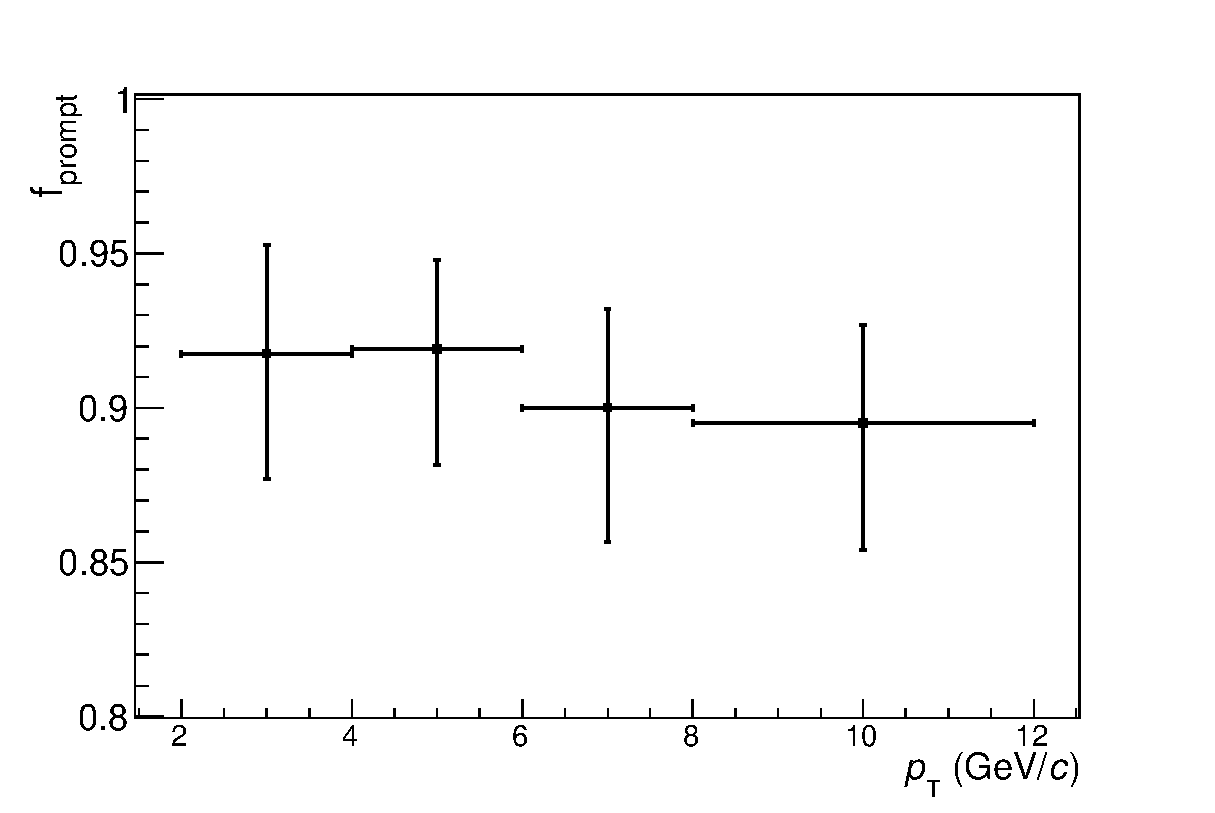
\includegraphics[width=.49\textwidth]{FigCap4/promptFraction_pass4.eps}
 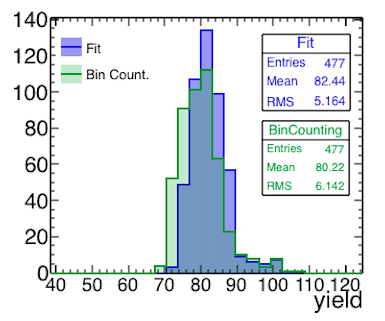
\includegraphics[width=.47\textwidth]{FigCap4/MT_pt68.png}
\caption{Left: prompt fraction values for $\Ds$ meson with the final selections as a function of $\pt$ in pp collisions at $\s = 7$ TeV. Right: multiple-trial raw yield distribution from fit and bin counting extraction in different colours, as an example for the interval \mbox{$6 < \pt < 8 \, \Gevc$}.}
\label{fig:fpromptAndMT}
\end{center}
\end{figure}



\section{Systematic uncertainties}
\label{sec:systPP}
In this section the studies carried out to estimate the systematic uncertainties on the
 measurement of the $\Dsplus$ cross section as a function of $\pt$ are presented. 
 The contributions to the systematic uncertainty from the different 
 sources were studied separately and are described in the following.

\subsection{Raw yield extraction}
\label{sec:RawYieldSyst}
The value extracted for the yield depends on the  
configuration of the invariant-mass fit.
In order to estimate the systematic uncertainty on the raw yield,
a possible approach is to explore all the possible fit configurations and build
a distribution of the yields, via a multiple-trial approach. The fits to the invariant-mass 
distributions were repeated several times varying
i) the lower and upper limits of the fit, 
ii) the background fit function (3 cases: exponential, linear and second 
order polynomial), iii) the Gaussian mean and width of the signal line shape, 
which were left free or fixed to MC
values. The fits which did not converge or had $\chi^2$/ndf $>$ 2.0 
were rejected and not considered in the evaluation of the 
systematic uncertainty. It was verified that the yields extracted with the
default fit parameters had compatible values to the mean of
the distribution of yields from the multiple-trial approach. 
An example of the distribution of yields from multiple-trial approach applied on fit and on
bin counting is shown in the right panel of Fig.~\ref{fig:fpromptAndMT},
for the interval $6 < \pt < 8 \, \Gevc$. 
In the blue distribution, the signal extraction is done via a fit of the invariant mass, while
in the green distribution it is estimated from the counting of the entries in the invariant-mass histogram after 
subtracting the background counts calculated from the 
background fit function.
The values of the mean and the RMS
of both the distributions are reported in the plot.
The RMS of the distribution of the multiple trials was used as an estimator of
the systematic uncertainty on the raw yield extraction. With the above
selection criteria, the value resulted to be $\sim$6\% in all $\pt$ intervals.
The relative difference between the means of the distributions
for the extraction via fit and via bin counting resulted
to be smaller than 6\% at all $\pt$ and therefore no additional uncertainty was assigned from this check. 
The assigned uncertainty is reduced by a factor 3-4 with respect to the analysis with the old reconstruction,
where it was around 15-20\% depending on the $\pt$ interval. 
To further investigate whether the systematic uncertainty estimated with
this approach is not too much conservative, a slightly
different approach was tested. We assumed that 
the systematic uncertainty on the yield extraction via the fit procedure 
arises only from variations in the line shape of the signal and 
in the fitting function for the 
background. Let us examine these two contributions separately.\\

\emph{Signal line shape}
The uncertainty from signal line shape was calculated by 
considering the combinations among these fit
configurations: (i) free Gaussian width parameter, (ii) width parameter 
fixed to MC value, (iii) Gaussian width varied by 20\% with 
respect to MC value (to account for the maximum difference of width values between data and MC), 
(iv) free peak position, (v) peak position fixed to MC value.
The uncertainty was estimated as the maximum error (max. value - min. value) divided by $\sqrt{12}$,
considering the distribution uniform.
It resulted to be $\sim$5\% in all the $\pt$ intervals. 

\begin{figure}[!hb]
\begin{center}
 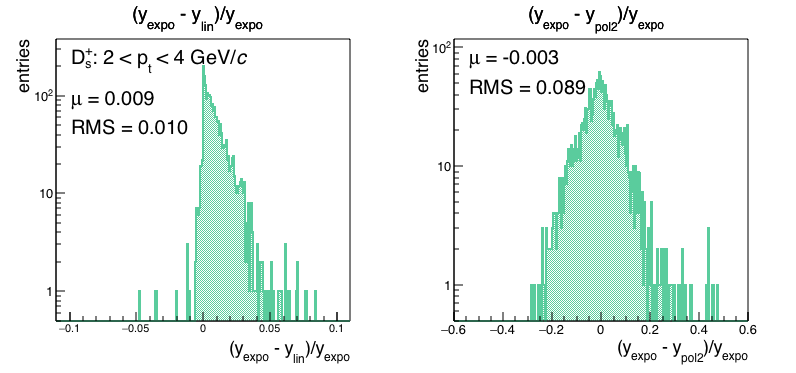
\includegraphics[width=.70\textwidth]{FigCap4/studyBkg_Free_pt0.png}
\caption{Relative difference of signal yield with exponential and first (left) and second (right) 
order polynomial functions for background, in $2 < \pt < 4 ~\Gevc$.}             
\label{fig:diffBkgPt0}
\end{center}
\end{figure}


\emph{Background fit function}
Using different functions to fit the background introduces 
some systematic differences in the extracted yields.
The default shape used for the central value of raw yield is an 
exponential function, but first and second 
order polynomial shapes were also tested to estimate the systematic 
uncertainty. In Table~\ref{tab:chi2bkg} 
the values of reduced chi square referred to the compatibility 
of the background function with data (excluding the region within 3$\sigma$ from the peak) are 
reported. 
\begin{table}[!h]
\centering
\vspace{0.5cm}
\begin{tabular}{|c|c|c|c|c|} 
\hline \rule{0pt}{2.7ex}
 & $\pt$ interval & Exponential & Linear & Pol2 \\ 
 &(GeV/$c$) & & &  \\ 
\hline \rule{0pt}{2.7ex}
           &\phantom{0}2--4\phantom{0} & 1.21 & 1.21 & 1.09\\
           $\chi^2/ndf$ &\phantom{0}4--6\phantom{0} & 1.15 & 1.18 & 1.16\\
          &\phantom{0}6--8\phantom{0} & 1.03 & 1.02 & 1.03\\
           &\phantom{0}8--12 & 0.99 & 0.99  & 1.03\\
\hline
\end{tabular}
\caption{Reduced $\chi^2$ values for the fit of the background (peak region excluded) in the
considered $\pt$ intervals of the $\Ds$ meson.} 
\label{tab:chi2bkg}
\end{table}
One can see that all the three shapes 
give a good description of data, but in general no improvements 
are visible when adding more parameters in the fit
with respect to exponential shape, so the latter confirms itself as a good choice.
Neverthless, it is important to look also at the values of the 
extracted yield to assess possible biases.
 In order to do this, 50 simulated samples were generated via 
 Poissonian smearing of the fit function with the exponential background.
 For each sample, the yields extracted utilising a fit function with exponential 
 background were compared with those obtained using linear and 
 polynomial functions with the same
configuration for the parameters of the Gaussian peak, mass range and bin width. The
difference of the yields with linear and parabolic backgrounds relative to 
the yield extracted using a fit with exponential background 
was used to fill a histogram. The procedure was repeated for different
configurations of lower and upper limits for the fit and 
invariant-mass bin widths for each of the
50 samples. 
A potential shift from zero of the mean of the resulting distribution 
 should reveal the bias from the change of background. The
  spread of the distribution is related to statistical fluctuations. 
  In Fig.~\ref{fig:diffBkgPt0} an example of the above 
  described distribution is presented, in the interval $2 < \pt < 4\, \Gevc$.
  Left and right panels show respectively the distribution of the difference
  of yields extracted with first or second order polynomial shapes to those extracted with exponential
  background. The shift in the distribution is not statistically significant 
 since $\mu < 3\,$RMS. Hence, no bias arises from the change of background
 and the main systematic effect from this approach comes from the function used for the 
 signal peak, resulting in a 5\% uncertainty that is consistent with the 6\% quoted from the first approach.\\
 
 
\begin{figure}[!h]
\begin{center}
 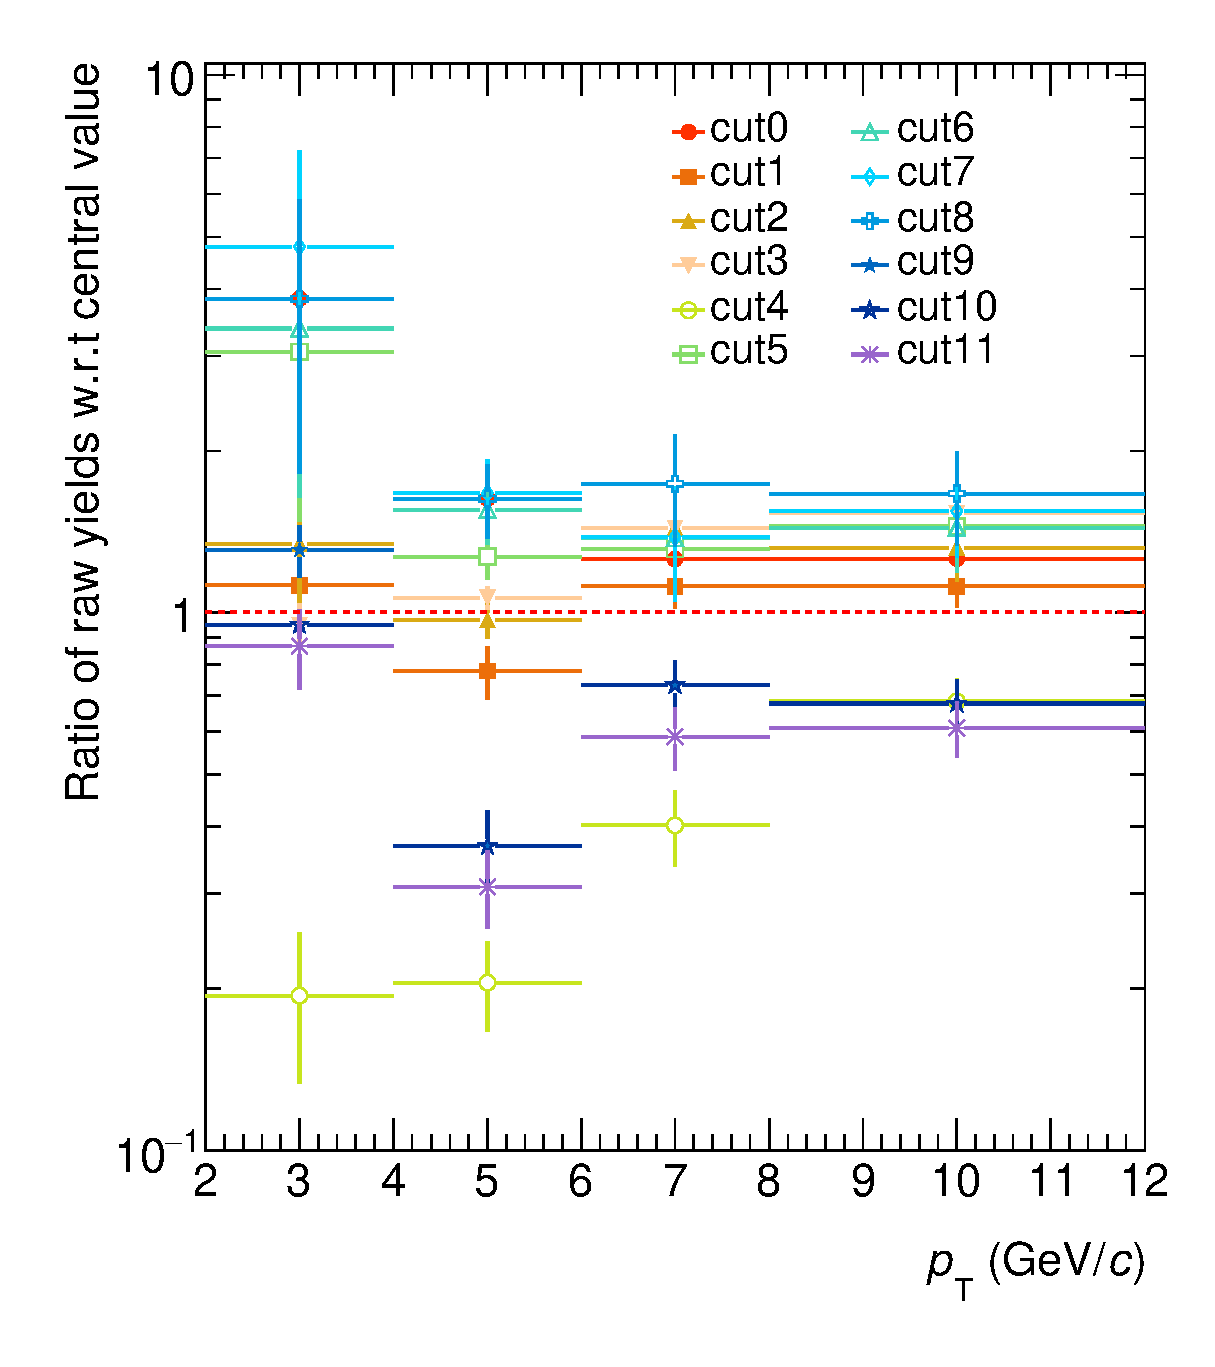
\includegraphics[width=.49\textwidth]{FigCap4/cutVariationPlot_pass4_rawY.eps}
 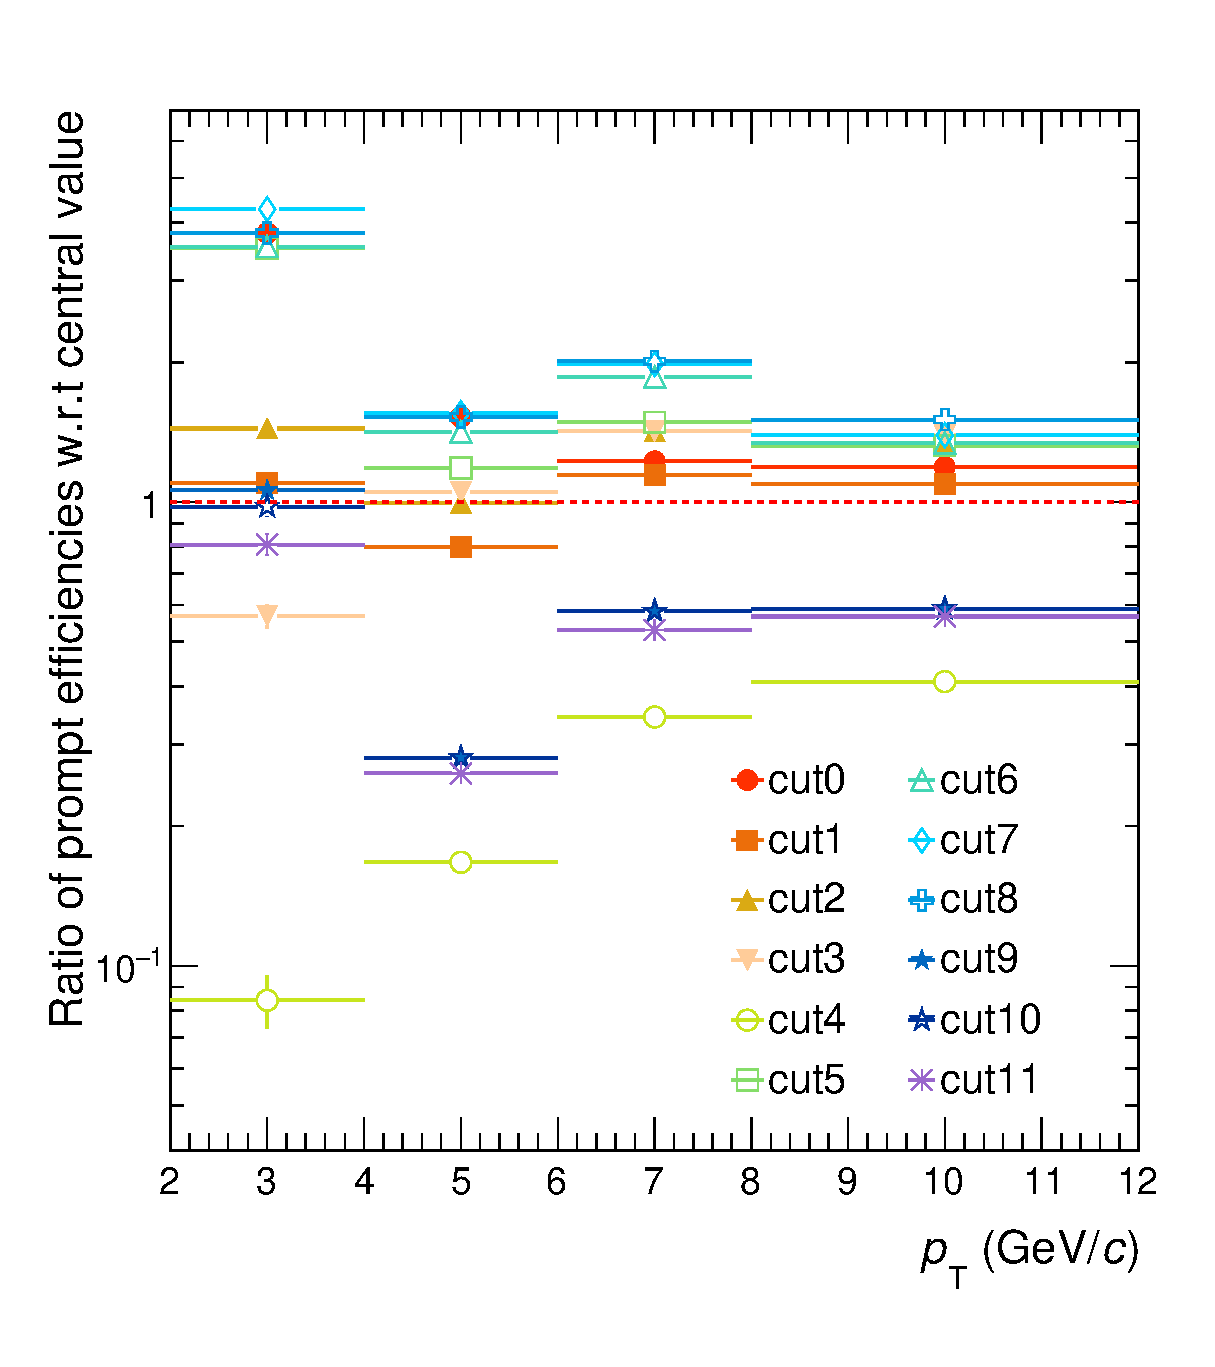
\includegraphics[width=.49\textwidth]{FigCap4/efficiencies_cuts0to12.eps}
 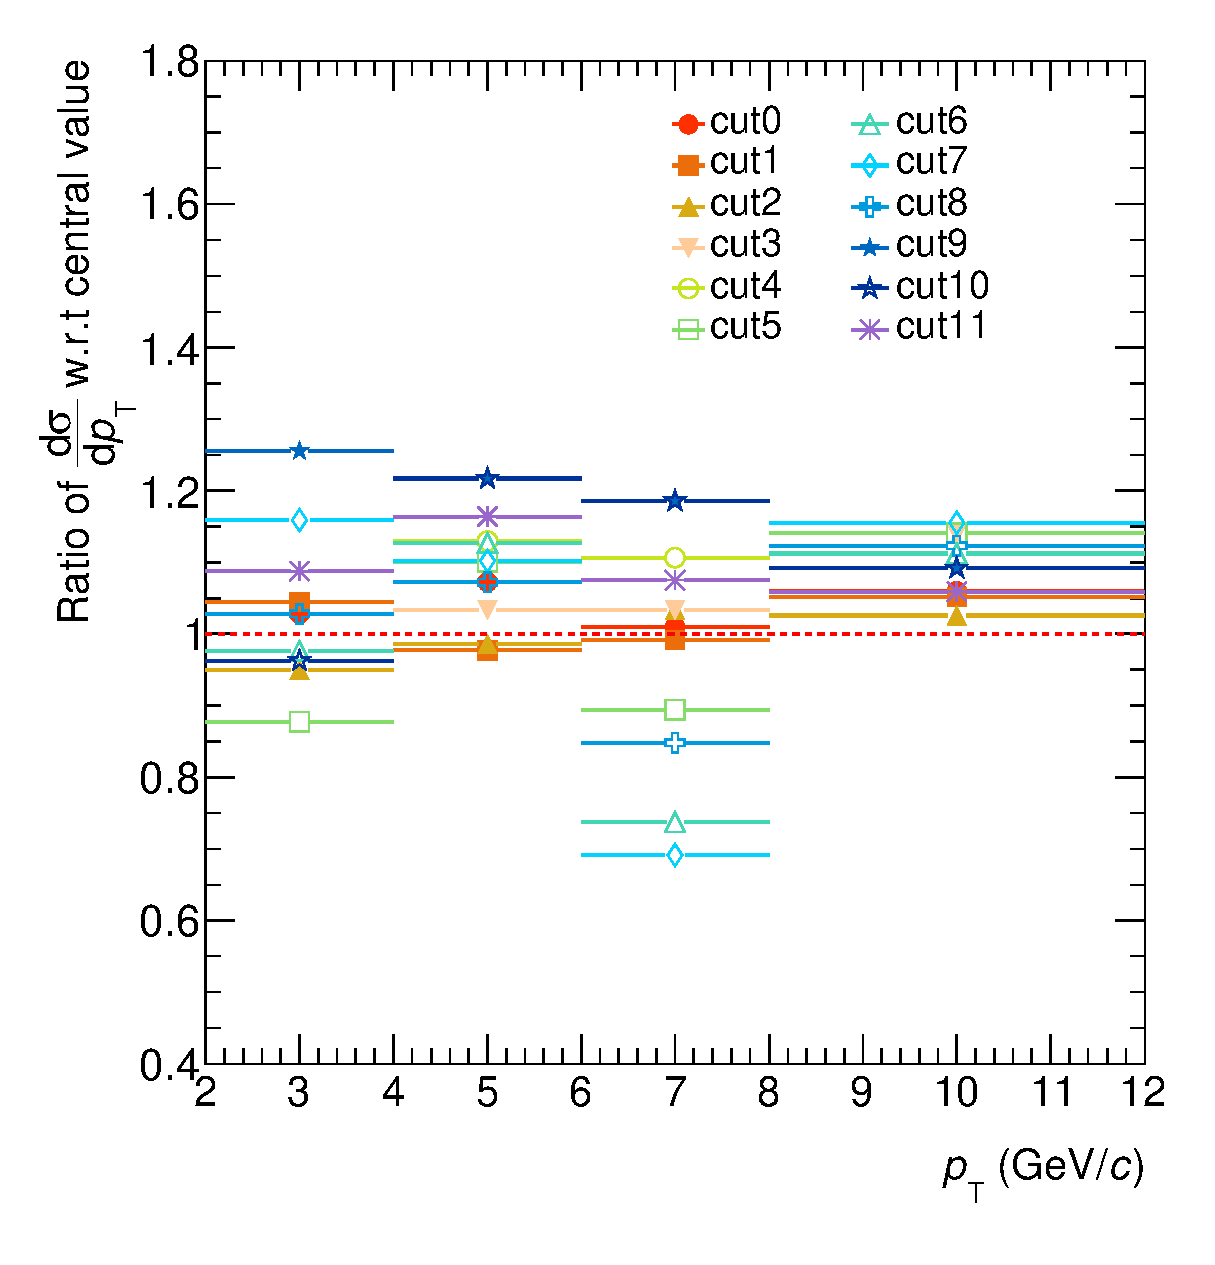
\includegraphics[width=.49\textwidth]{FigCap4/cutVariationPlot_pass4.eps}
\caption{Ratios of $\Ds$ raw yields (top left), selection efficiencies (top right) and cross sections (bottom) with different sets of cuts with respect to their respective values with the default selections, as a function of $\pt$.}             
\label{fig:cutVar}
\end{center}
\end{figure} 
\subsection{Selection efficiency}
\label{sec:CutVariation}
The systematic uncertainty on the selection efficiency accounts for 
possible imperfections in the MC description of the variables used to select the signal, 
which could introduce a bias in the efficiency. A possible test to quantify the effect of any discrepancy in the 
description of topological variables between data and MC is to exploit different sets of cuts
that have different selection efficiencies and to compare the cross sections.
In this analysis, twelve sets of cuts were compared, 
their respective efficiencies spanning a variation up to 
a factor of $\sim$6 with respect the default efficiency, depending on the $\pt$ interval.
Only the cuts that provided 
medium-high statistical significance and good S/B ratios of the extracted yields
were taken into account for the final systematics.
Fig.~\ref{fig:cutVar} shows the ratios of raw yields (top left panel) and efficiencies (top right) 
extracted with the different sets of cuts with respect
to the reference values with the default selections as a function of $\pt$.
To find several sets of cuts that provide a good signal stability, 
more than one variables need to be varied at the same time. It is very likely that,
while the selection on some variables needs to be released, the selection
on others requires to be tightened. For this reason, the extracted yields with lower selection efficiency are in general not simply
sub-samples of those with higher efficiency, thus making not straightforward the calculation
of the error on the ratios of raw yields and hence, of the cross sections in order to
estimate the systematic uncertianty.
The ratios of the different cross sections to the default one are shown in the bottom panel of the
same Fig.~\ref{fig:cutVar}. We took the RMS of the their distributions in each $\pt$ interval as an estimator of 
the systematic uncertainty. The uncertainty resulted to be 7\% in all $\pt$ bins.
\begin{figure}[!h]
\begin{center}
 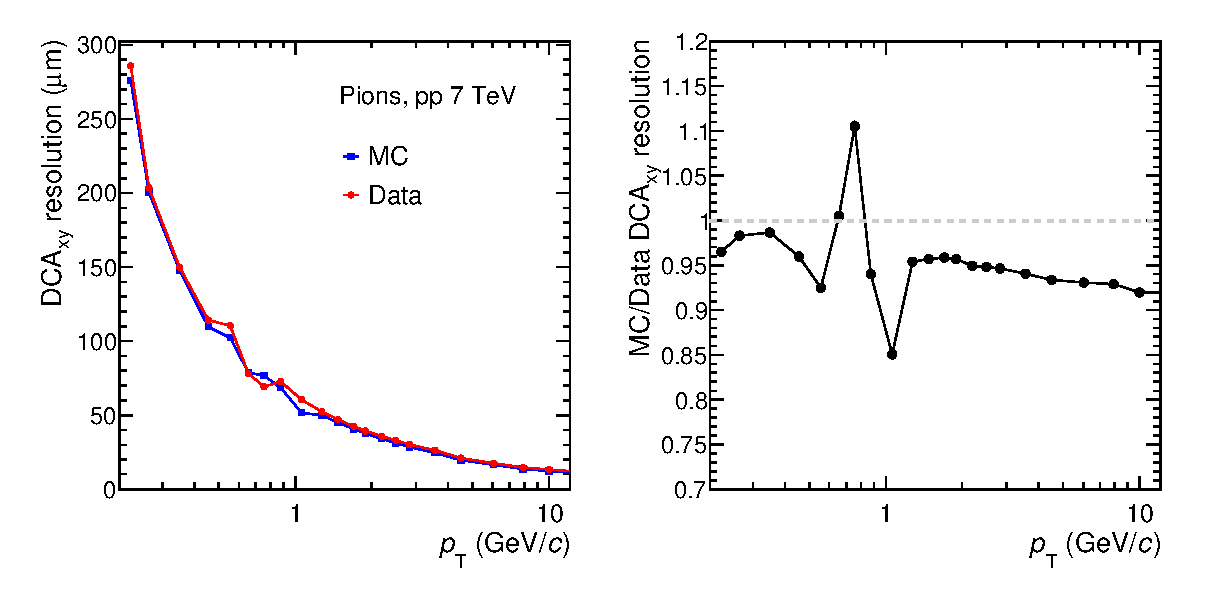
\includegraphics[width=1\textwidth]{FigCap4/DCAxyReso_Pions.eps}
\caption{DCA$_{\rm xy}$ resolution curves of pion tracks as a function of $\pt$ in data and in MC (left panel) and their ratio (right panel) in pp collisions at $\s = 7 $ TeV.}             
\label{fig:DCAxyReso}
\end{center}
\end{figure}
In particular, the effect of possible imperfections in the description 
of the residual misalignment in the simulations was studied separately 
starting from the differences observed on the impact parameter resolution
in data and in the simulation.
Fig.~\ref{fig:DCAxyReso} (left) shows, as an example for pion tracks, distributions of
DCA$_{\rm xy}$ resolution as a function of $\pt$ in data and in simulation 
in pp collisions at $\s = 7 $ TeV. The values were extracted via fits to the DCA$_{\rm xy}$ distributions
of tracks in data and in MC, in different $\pt$ intervals. 
The right panel of the Fig.~\ref{fig:DCAxyReso} shows the 
MC-to-data ratio of the DCA$_{\rm xy}$ resolutions. 
The agreement is overall good. To estimate the effect of the residual discrepancy,
the resolution values in the MC were reduced by 10\% and the
DCA$_{\rm xy}$ of tracks in MC smeared according to the new resolution.
The variation of the efficiencies was less than 3\%, lower
than the 7\% from the cut variation study, which includes this contribution.
\iffalse
\begin{figure}[!htb]
\begin{center}
 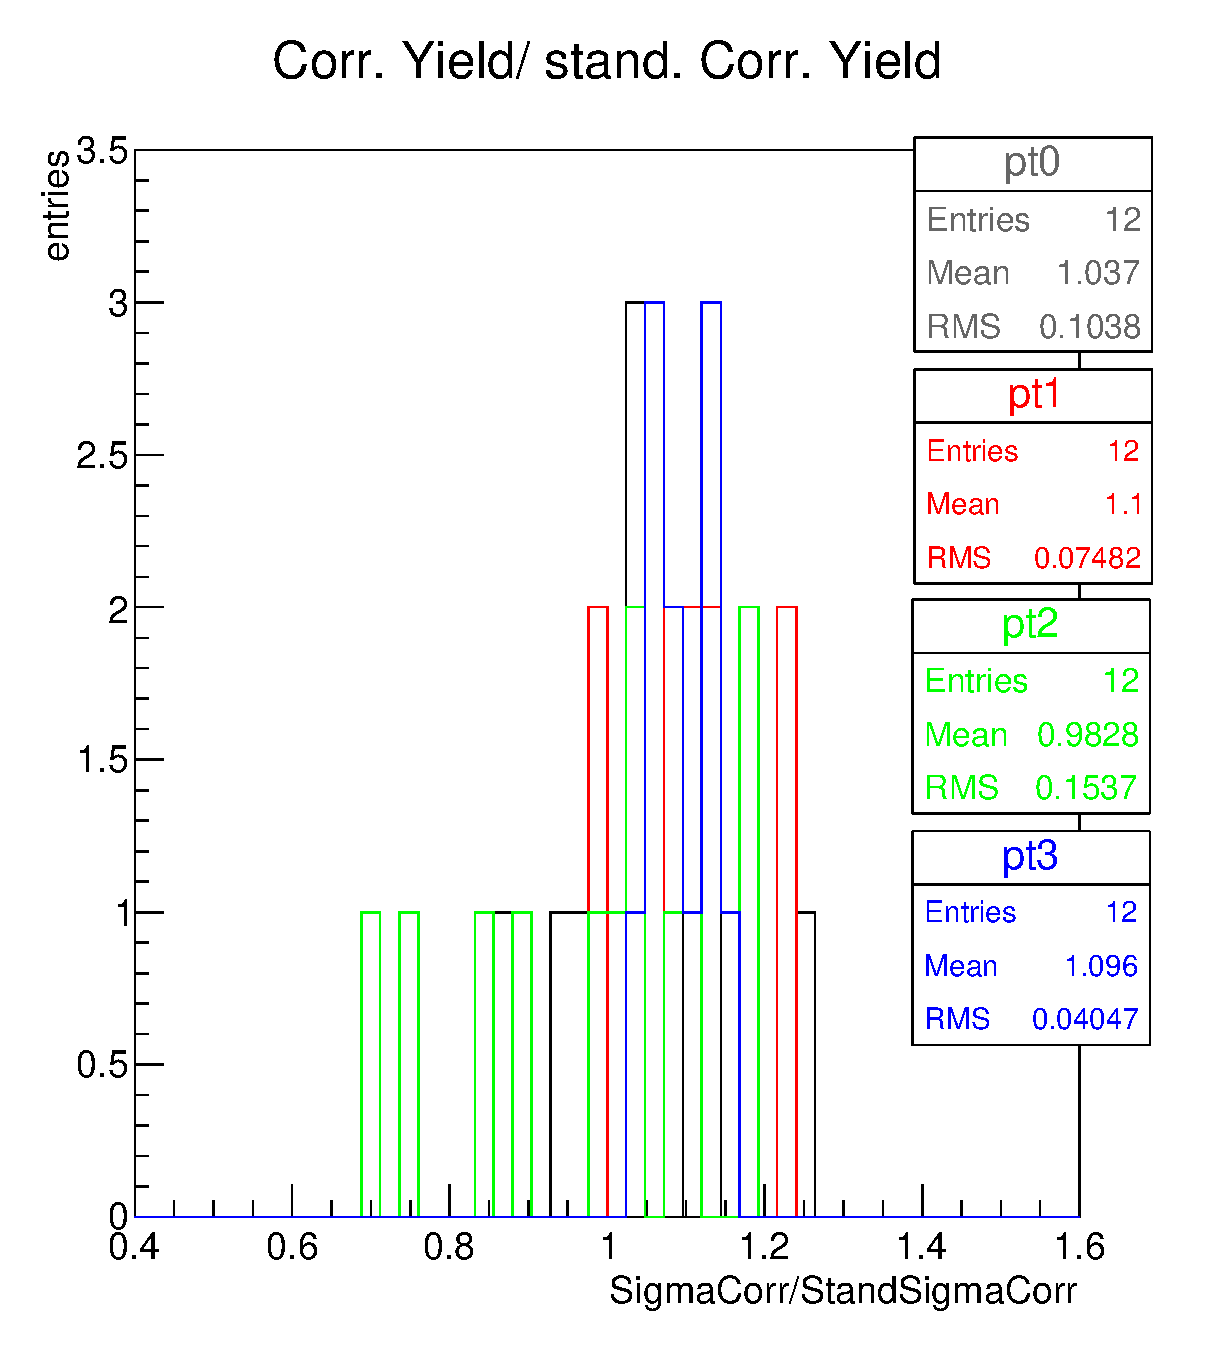
\includegraphics[width=.44\textwidth]{FigCap4/rms_cutvariation.eps}
 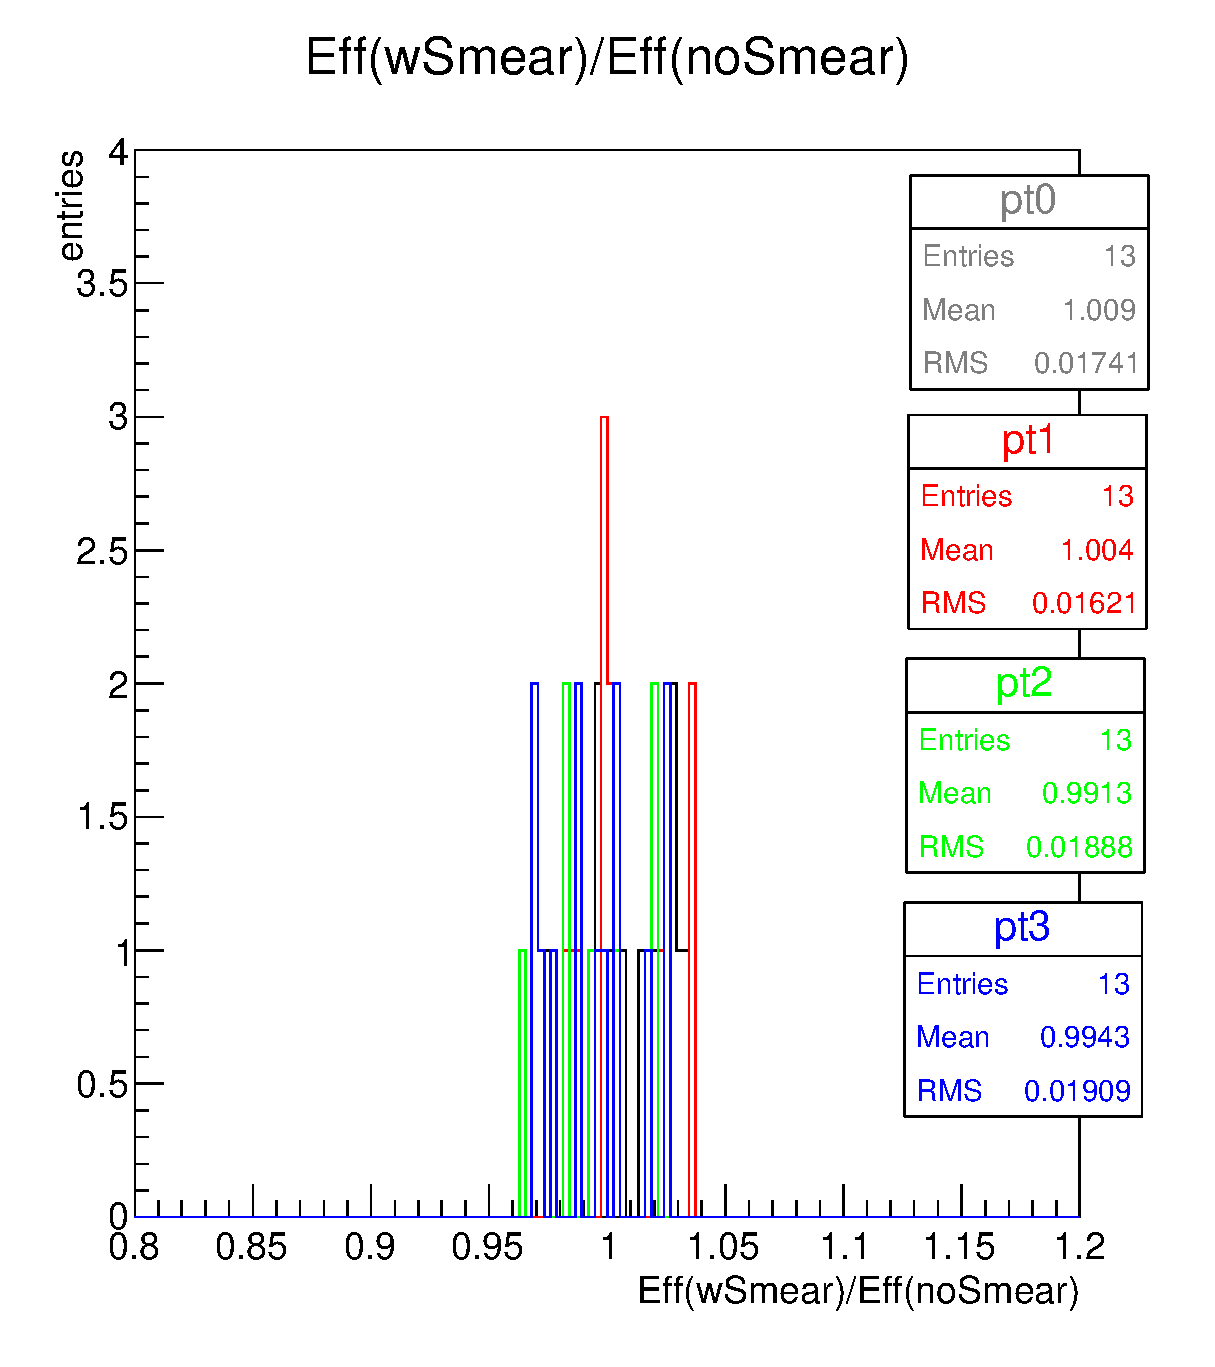
\includegraphics[width=.44\textwidth]{FigCap4/rms_smearp10.eps}
\caption{Left: $\Ds$ corrected yield measured with 12 different sets of
cuts and compared to the yield from the best set of cuts (chosen for the central yield value). Right: ratio for $\Ds$ efficiencies w/o a 
10\% smearing on the xy impact parameter resolution.}             
\label{fig:cutVariation}
\end{center}
\end{figure}
\fi

\subsection{PID efficiency}
\label{sec:PIDsystPP}
To test the efficiency correction of PID efficiency, looser PID selection criteria were
used with respect to the default selection described in Sec.~\ref{Sec:PID}. 
In fact, in the $\Ds$ case, the rare signal and the large background 
do not allow for a reliable signal extraction without 
particle identification. The looser PID selection accepts those cases 
reported in Fig.~\ref{fig:strongPID} where combined response values from TPC and TOF 
detectors are 0, 1 or 2, which correspond to a 3$\sigma$ cut on the d$E$/d$x$ and
time-of-flight signals. The tighter standard selection only accepts as final
response values of the tracks 1 or 2.
In Fig.~\ref{fig:rmsPID} the ratio
of the corrected yields obtained with looser-to-default PID selection is shown, 
for the twelve different sets of cuts discussed in Sec.~\ref{sec:CutVariation}.
The evaluation of the systematic uncertainty, estimated as the RMS of the distributions in each $\pt$ 
interval, was made considering only the region $\pt > 4 \, \Gevc$, since 
with looser PID we could not obtain a stable extraction of the raw yield for most
of the different sets of cuts, whose statistical significance values were $<3$ and the S/B was about few percent.
The RMS of the corrected yield distributions for the considered
$\pt$ intervals is about 7\% and this value is assigned as uncertainty in all $\pt$ intervals.

\begin{figure}[!htb]
\begin{center}
 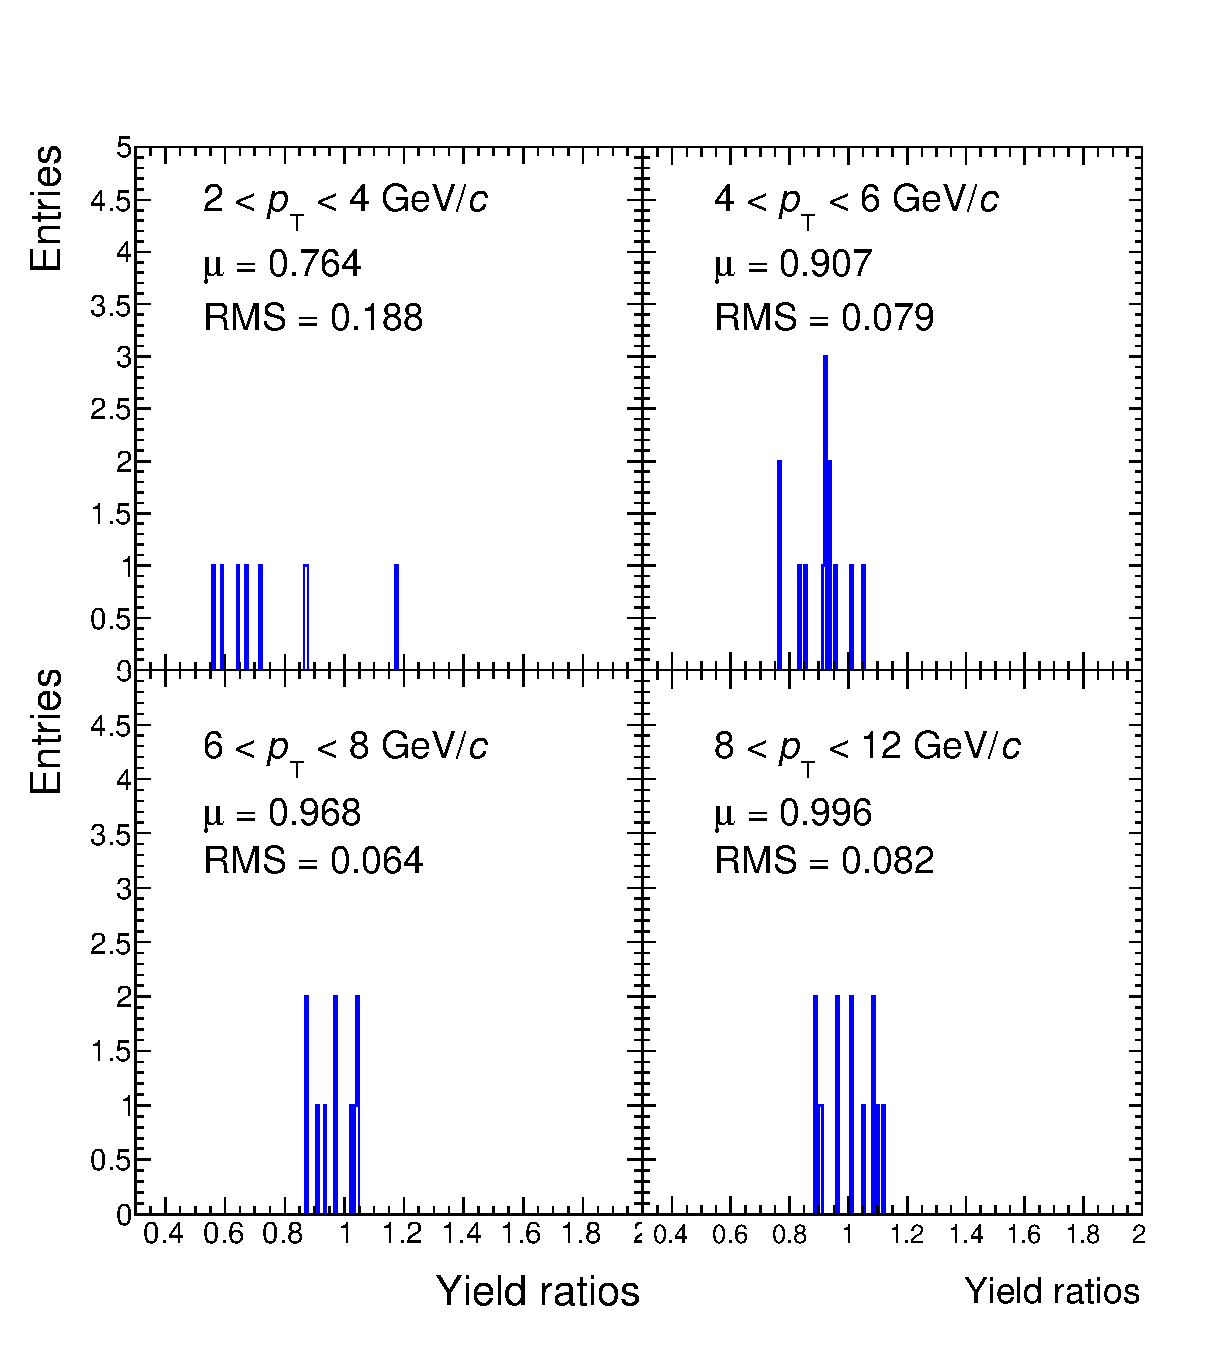
\includegraphics[width=.7\textwidth]{FigCap4/PIDrms4x4}
\caption{Ratio of $\Ds$ corrected yields with looser and default PID selections (for twelve different sets of
topological selections).}
\label{fig:rmsPID}
\end{center}
\end{figure}

\subsection{Track reconstruction efficiency}
\label{sec:TrackEffSystPP}
The systematic uncertainty related to the tracking efficiency includes the 
effects arising from track finding in the TPC, from track prolongation  
from the TPC to the ITS, and from track quality selections.
It was estimated with the following tests:
\begin{itemize}
\item comparison of the D-meson cross sections obtained with different track selection cuts;
\item comparison of the TPC-ITS track matching efficiency in data and simulations.
\end{itemize}
These checks are discussed in the following subsections.

\subsubsection{Variation of track selections}
\label{subsec:trackEffpp}
For this purpose, $\Dzero$ and $\Dplus$ mesons were used due to their
higher statistical significance of the extracted yields.
The D-meson raw yields and efficiencies were evaluated with 
different sets of track selection cuts.
The following selections were tested:
\begin{enumerate}
\item additional cut on number TPC crossed rows $> 120$-$[5\, ( \Gevc )/\pt]$ (not used in the default selections);
\item additional number of TPC clusters $>0.65 \times$ number of TPC crossed rows (not used in the default selections);
\item tighter selection on the ratio of crossed rows over findable clusters in the TPC ($>0.9$ instead of 0.8).
\end{enumerate}
The systematic uncertainty was assigned based on the observed variation of
the prompt $\Dzero$ and $\Dplus$ cross sections with respect to the default selections.
Based on this check, systematic uncertainties of 2\% and 3\% independent of D-meson $\pt$ were 
respectively estimated for $\Dzero$ (two-body decay) and $\Dplus$ (three-body decay). 
The values are consistent with a 1\% per-track systematic
uncertainty, that was inherited for the $\Ds$-meson analysis.

\subsubsection{ITS-TPC matching efficiency}
\label{sec:MEpp}
The matching efficiency, i.e. efficiency of track prolongation from TPC to ITS, 
is defined as the fraction of tracks successfully prolonged from TPC to ITS (having
at least one cluster in the SPD layers)
over the number of tracks reconstructed in TPC.
Systematic uncertainty on its determination arises from discrepancies 
in the tracking performance between data and Monte Carlo.
Primary particles are defined as 
prompt particles produced in the collision, including decay products, 
except those from weak decays of strange particles. Matching efficiency for primary tracks is higher than 
for secondary tracks (originating from strange-hadron decays, thus 
with secondary vertices likely to be outside the SPD layers or for particles produced
in interactions with material). 
If the fractions of primary and secondary tracks are different in data 
and in Monte Carlo, this could lead to a discrepancy in the matching efficiency
which is not due to the tracking performance and therefore it should not be
accounted in the systematic uncertainty on tracking. Hence,
data-driven corrections for primary and secondary fractions were used to re-weight the MC
and obtain a corrected inclusive MC efficiency, which is then used in the
comparison to data, to estimate the systematic uncertainty.\\
The steps in the procedure are:
\begin{itemize}
\item extract the matching efficiencies for different particle types: 
Eff$^{\rm MC}_{\rm primaries}$, Eff$^{\rm MC}_{\rm secondaries}$, Eff$^{\rm Data}_{\rm inclusive}$
\item extract the fraction of primary tracks in data: f'$_{\rm primaries}$
\item compute a corrected MC-inclusive efficiency: 
Eff$^{\rm MC}_{\rm inclusive}$ = f'$_{\rm primaries}$ x Eff$^{\rm MC}_{\rm primaries}$ + (1- f'$_{\rm primaries}$) x Eff$^{\rm MC}_{\rm secondaries}$
\item estimate the relative systematic uncertainty: 
(Eff$^{\rm Data}_{\rm inclusive}$ - Eff$^{\rm MC}_{\rm inclusive}$)/Eff$^{\rm Data}_{\rm inclusive}$.
\end{itemize}
A minimum-bias Monte Carlo production (with the PYTHIA 6 event generator and
GEANT 3 for particle transport through the apparatus) anchored to 2010 pp data taking at 
$\s = 7$ TeV was used for this study. Charm-enriched productions were not used in this study 
since the shape of DCA distribution of tracks (used to extract data-driven 
primary track fraction) is affected by the heavy-flavour particle enhancement
and may bias the fit.
Efficiency was studied as a function of:
\begin{itemize}
\item $\pt$, from 0.5 to 15 $\Gevc$
\item $\phi$, between (0,2$\pi$)
\item $\eta$, between (-0.8,0.8)
\end{itemize}

Let us examine below more in detail the steps needed to 
calculate the systematic uncertainty.
\begin{enumerate}
\item {\bf ITS-TPC matching efficiency:} it is calculated separately for 
primary and secondary tracks in MC, inclusively on data. For 
the numerator of the matching efficiency, tracks were selected requiring 
to have a successful fit with the Kalman filter in the TPC and ITS, a hit in one of the two SPD layers, 
$|$DCAxy$|<$ 2.4 cm and $|$DCAz$|<$ 3.2 cm.
\begin{figure}[!htb]
\centering
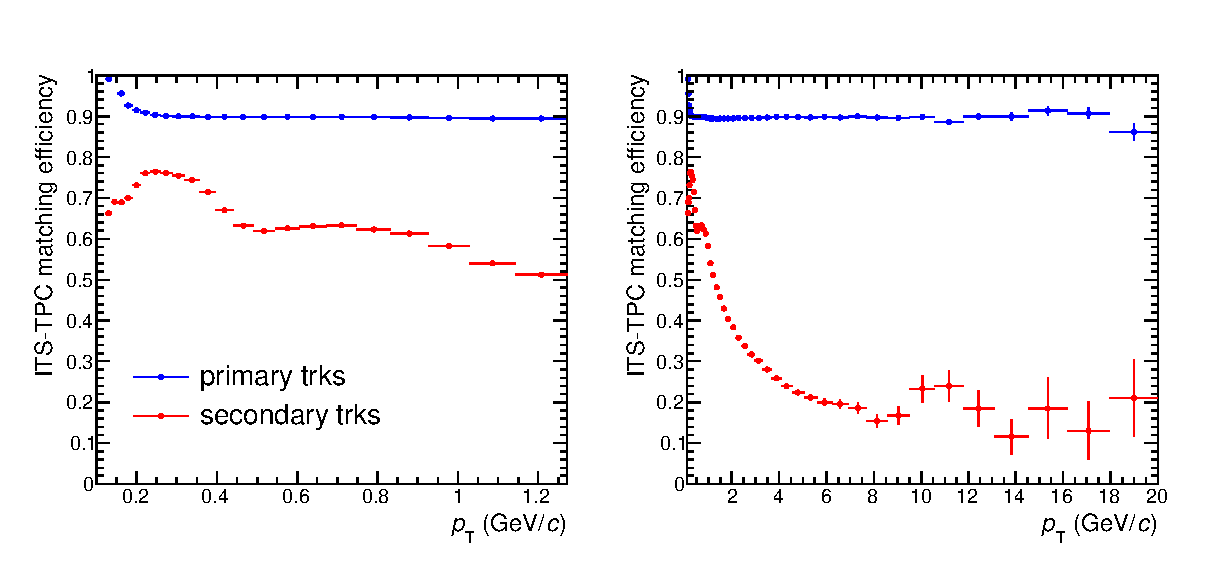
\includegraphics[width=1\textwidth]{FigCap4/ITSTPC_matchEff_vsPt_LowFullpt.eps}
\caption{Matching efficiency for primary and secondary tracks as a function of $\pt$ in MC for $\pt$ interval from 0.1 to 1 $\Gevc$ (left) and up to 20 $\Gevc$ (righ). }
\label{fig:matcheff_pt}
\end{figure}

In Fig.~\ref{fig:matcheff_pt}, ITS-TPC matching efficiency 
of charged tracks in MC as a function of 
$\pt$ is shown. The left panel is referred to the low $\pt$ region (0.1-1 $\Gevc$), 
the right one extends the $\pt$ interval up to 20 $\Gevc$. 
The difference between matching efficiency of primary and secondary tracks
is large and increases with $\pt$.

\item {\bf Fractions of primary tracks:} they are extracted with a data-driven technique based on a fit to
 the measured track impact parameter distribution using MC templates for 
 DCA$_{\rm xy}$ distributions of primary and secondary tracks, in different
 $\pt$, $\eta$ and $\varphi$ intervals. The ROOT TFractionFitter 
 package was used to perform the fit. The fit was configured 
 using three templates describing primary tracks, secondaries tracks
 from strange-hadron decays and tracks produced in interactions in the material. 
 A selection on tracks requiring at least one hit in either of the two SPD layers 
 was used, to assure good enough resolution to distinguish primary and 
 secondary DCA$_{\rm xy}$ distributions.
\begin{figure}[!htb]
\begin{center}
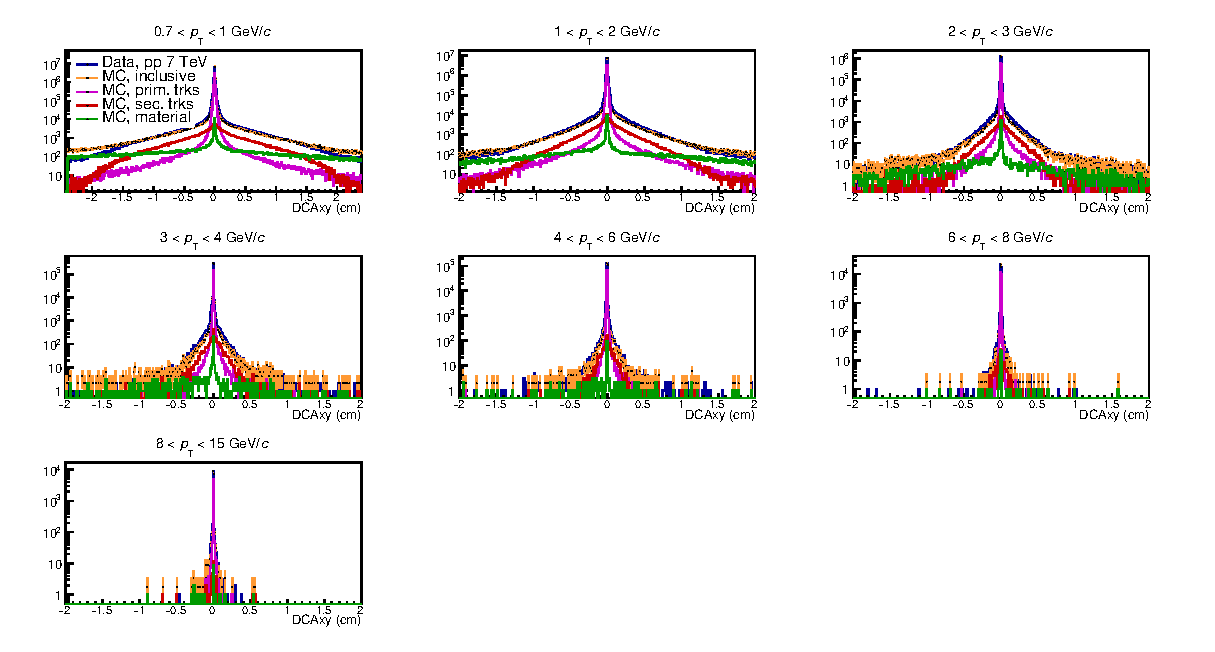
\includegraphics[width=1.2\textwidth]{FigCap4/FitComponents.eps}
\caption{DCA$_{\rm xy}$ distributions in data and in MC for primary and secondary tracks in different colours, in $\pt$ intervals from 0.5 to 15 $\Gevc$.}
\label{fig:DCAxyDataMCVsPt}
\end{center}
\end{figure}
\begin{figure}[!hb]
\begin{center}
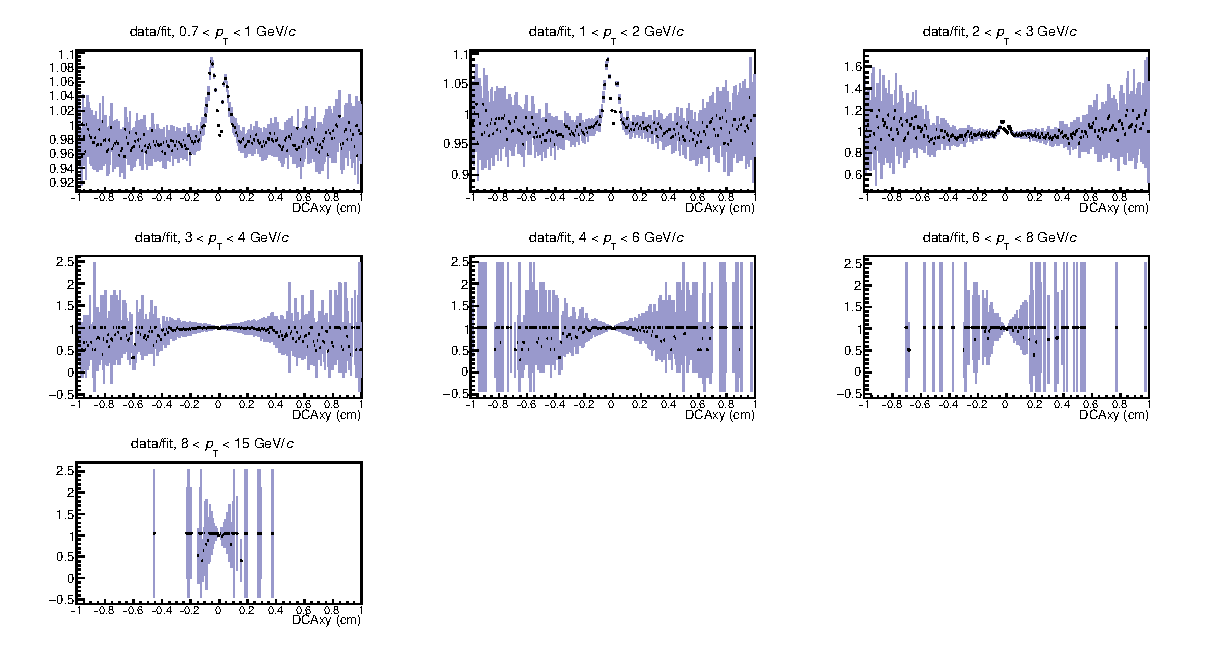
\includegraphics[width=1.2\textwidth]{FigCap4/DataOverFit.eps}
\caption{Ratio of DCAxy distributions in data and in the fit result histograms, in $\pt$ intervals from 0.5 to 15 $\Gevc$.}
\label{fig:DCAxyRatioDataFitVsPt}
\end{center}
\end{figure}
Fits were performed on the DCA$_{\rm xy}$ distributions of charged particles from data
in the range [-1,1] cm, in different intervals of $\pt$, $\varphi$, $\eta$ 
and constraining the three fractions in the TFractionFitter class within reasonable minimum and maximum values.
The fractions were then calculated by integrating the histogram 
resulting from the fit in the range $|$DCA$_{\rm xy}|<$ 2.4 cm, for
consistency with what done for the matching efficiency calculation. 
As a closure test, it was verified that the MC values for the fractions of primary and secondary tracks 
were in agreement with the values extracted when performing the fit with TFractionFitter 
on the inclusive MC distribution, with the three MC templates.  
In Fig.~\ref{fig:DCAxyDataMCVsPt} the distributions of DCA$_{\rm xy}$ 
in data and in MC for the different components are
shown in different colours, in $\pt$ intervals from 0.5 to 15 $\Gevc$. 
In Fig.~\ref{fig:DCAxyRatioDataFitVsPt} the ratio of DCA$_{\rm xy}$ distributions 
in data to the distribution resulting from the fit (obtained as output of TFractionFitter class) are plotted.
At low $\pt$, where the statistics allows a good performance of the fit, 
the values of the bin-per-bin ratios stay within 10\% variation. At higher $\pt$,
the agreement gets slightly worse but the values of the ratios always stay 
around unity. Furthermore, the smooth values of the data-driven
fractions obtained from the fits as a function of $\pt$, $\eta$ and $\varphi$
are an indication of the reliability of the fit.
In Fig.~\ref{fig:Fractions}, the data-driven values of primary and secondary
 fractions are shown and compared to 
 the ones from the PYTHIA + GEANT 3 simulation (empty markers). 
The fraction of secondaries in the figure already includes the contributions 
from material. We conclude that the fraction of secondaries is underestimated in the simulations.
\begin{figure}[!hb]
\begin{center}
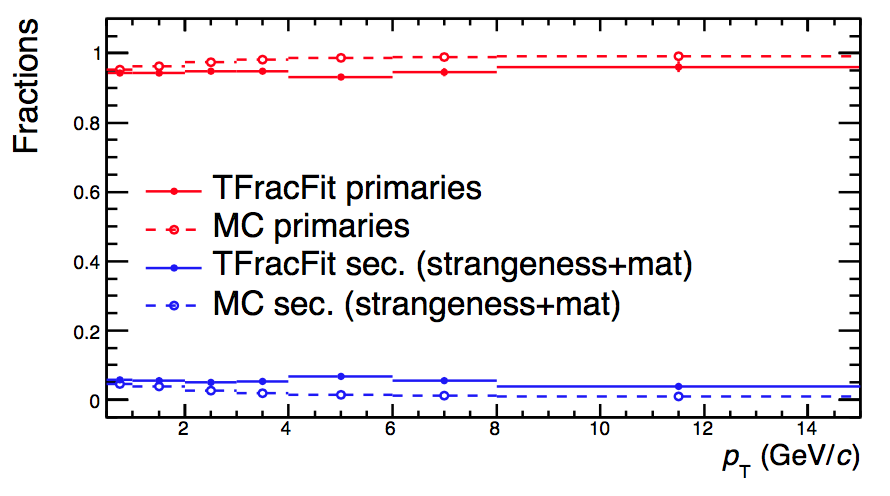
\includegraphics[width=.6\textwidth]{FigCap4/MEfractions.png}
\caption{Data-driven (solid lines) and MC (dashed lines) fractions of primary (red) and secondary (blue) tracks as a function of $\pt$ in pp collisions at $\s = $ 7 TeV.}
\label{fig:Fractions}
\end{center}
\end{figure}

\item {\bf Correction to the primary fraction:} since the fraction of primary
 particles was calculated using tracks with the request of a hit in one of the SPD layers, 
the primary fraction estimated for this sample of tracks 
needs to be rescaled to the primary fraction of the sample of tracks reconstructed in the TPC.
The reason for this correction is that the primary fraction is then used 
to (re)-weight the matching efficiency, that is normalised to the number of tracks in the TPC only. 
The fractions of primary tracks are expected to 
be different in ITS and TPC due to their different amount of 
secondary tracks from strangeness decays,
whose secondary vertices are likely to be outside the SPD layers. 
The correction factor is based on MC information and obtained as 
the ratio of the fraction of primary tracks in TPC to the fraction of primary
 tracks with TPC-ITS matching and one point in the SPD. The final fraction of primary tracks is hence
  f'$_{\rm primaries}$ = f$_{\rm primaries}$ x correction factor, 
  where f$_{\rm primaries}$ is the fraction obtained at step 2. 
  Typical values of correction factor for primary tracks are around $\sim$ 0.95-0.98
  as a function of $\pt$. 
  In Fig.~\ref{fig:MCfractions} an example of fractions of primary 
  and secondary tracks in MC requiring ITS-TPC matching or points in the TPC detector only are 
  shown in different colours as a function of $\pt$.
\begin{figure}[!htb]
\begin{center}
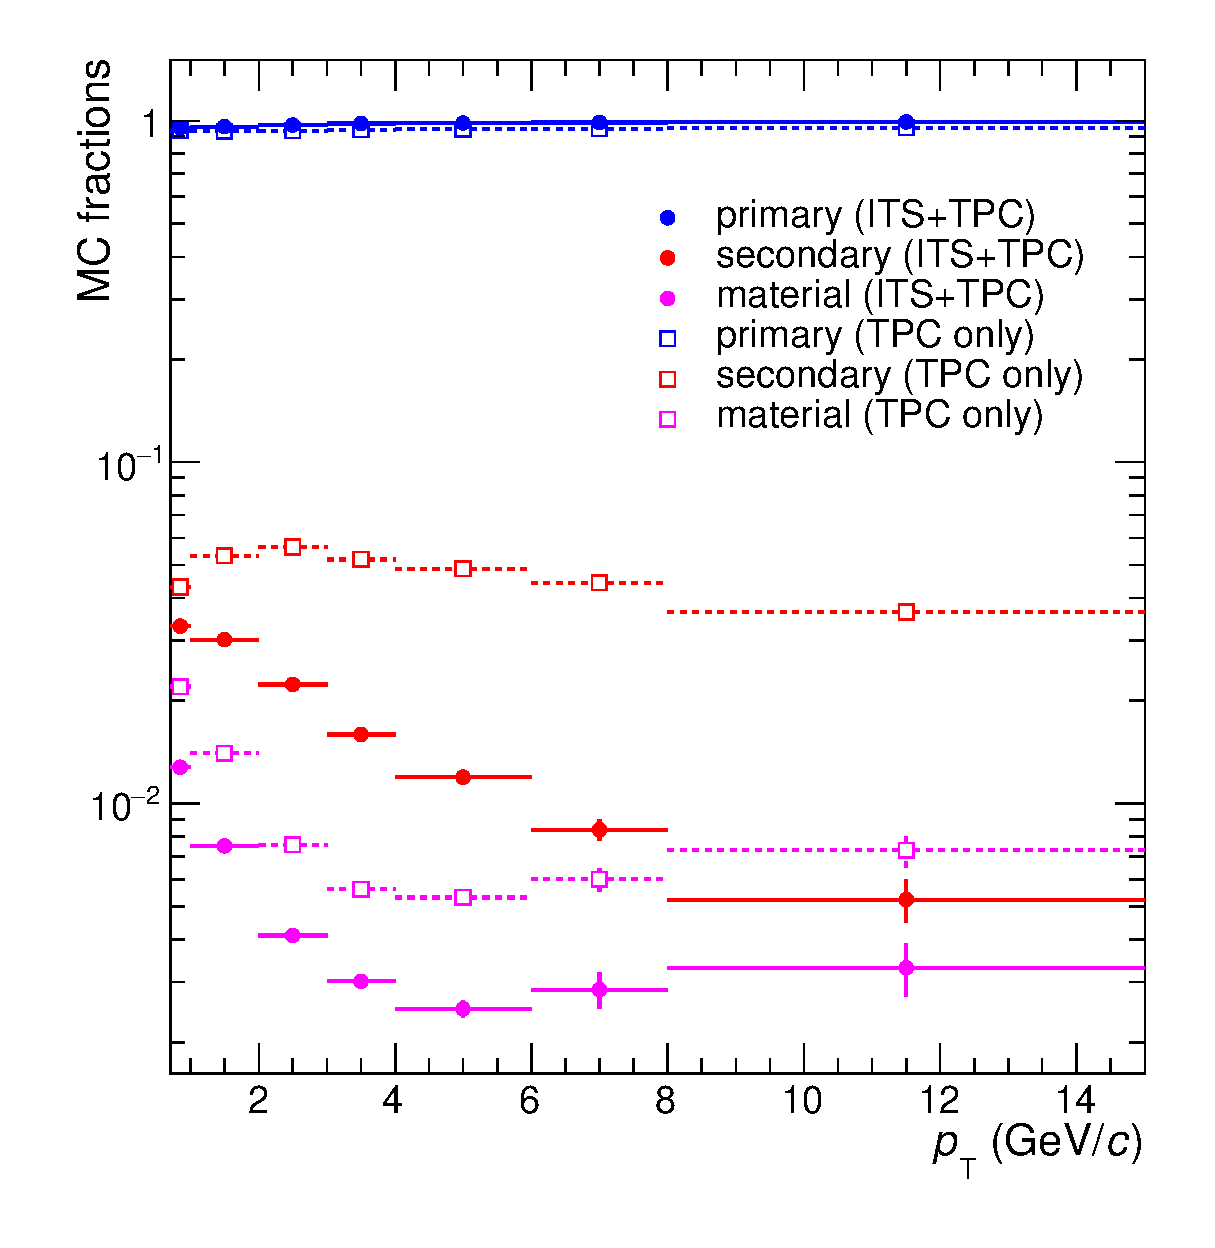
\includegraphics[width=.50\textwidth]{FigCap4/MCfractions_ESDTrOnly_VsPt_PiK.eps}
\caption{Example of fractions of primary and secondary tracks in MC requiring ITS-TPC and one point in SPD layers or TPC only selections in different colours as a function of $\pt$.}
\label{fig:MCfractions}
\end{center}
\end{figure}

\item {\bf ITS-TPC corrected matching efficiency:} it is calculated 
as  Eff$^{\rm MC}_{\rm inclusive}$ = f'$_{\rm primaries}$ x Eff$^{\rm MC}_{\rm primaries}$ + (1- f'$_{\rm primaries}$) x Eff$^{\rm MC}_{\rm secondaries}$. The corrected matching efficiency 
is shown in Fig.~\ref{fig:CorrMatchEffVsPt},~\ref{fig:CorrMatchEffVsPhi} 
(left) and~\ref{fig:CorrMatchEffVsEta} (left)
as a function of $\pt$, $\phi$, $\eta$ respectively, for kaons and 
pions (selected with a 3$\sigma$ PID cut on d$E$/d$x$ in TPC). 
It was verified that no substantial changes are obtained if 
considering all the species ($\pi, {\rm K, p, e,} \mu$). 
The drops in efficiency in some $\phi$ regions are due to SPD
inefficiencies during the data taking.
Finally, the ratios of MC inclusive (i.e. including primary and secondary tracks) matching efficiencies to
efficiency in data are shown in Fig.~\ref{fig:MatchEffSystVsPt},~\ref{fig:CorrMatchEffVsPhi} 
(right) and~\ref{fig:CorrMatchEffVsEta} (right) as a function of 
$\pt$, $\phi$, $\eta$ respectively. The data driven weighting procedure 
in MC allows to obtain better description of the data and a reduced systematic uncertainty
as compared to the one obtained using the uncorrected MC.
\begin{figure}[!htb]
\begin{center}
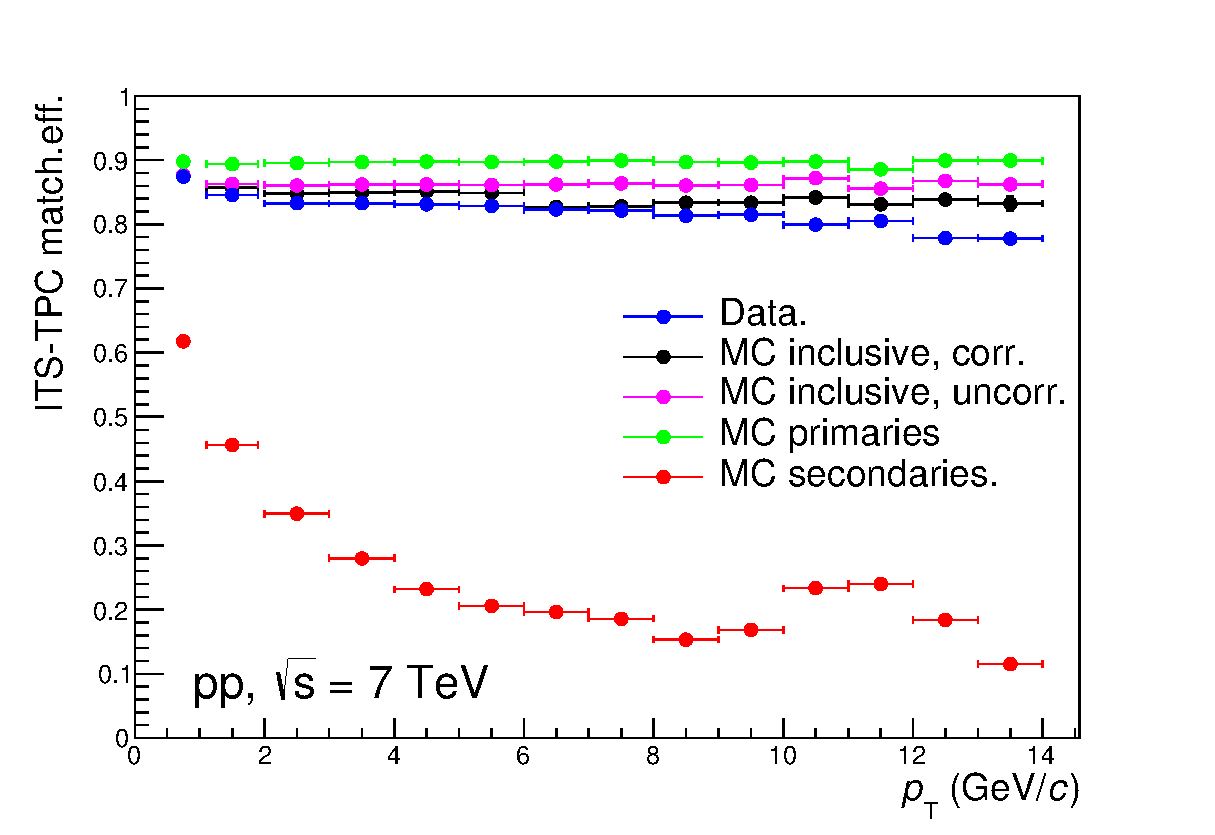
\includegraphics[height=7cm]{FigCap4/ITSTPCmatchEff_10bpass4_vsPt.eps}
\caption{ITS-TPC matching efficiency as a function of $\pt$ for 2010 pp data taking at $\s = 7$ TeV. The matching efficiency is shown for data (blu), for MC primary (green) and secondary (from strangeness decay and material interaction, in red) tracks, for inclusive MC tracks with (black) and without (magenta) data-driven correction. }
\label{fig:CorrMatchEffVsPt}
\end{center}
\end{figure}
\begin{figure}[!htb]
\begin{center}
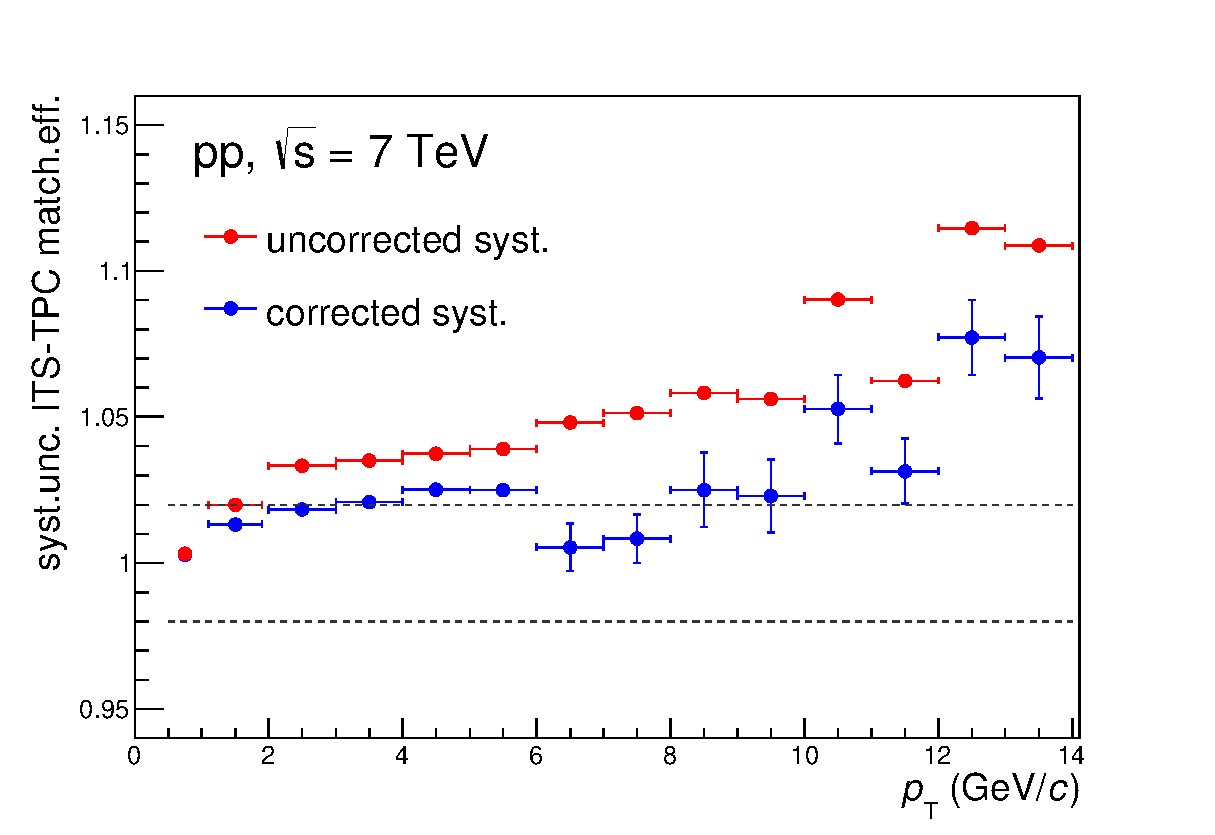
\includegraphics[height=7cm]{FigCap4/ITSTPCmatchEffSyst_10bpass4_vsPt.eps}
\caption{Ratio of ITS-TPC matching efficiencies in data and MC as a function of $\pt$ before (red) and after (blue) data-driven correction.}
\label{fig:MatchEffSystVsPt}
\end{center}
\end{figure}
This per-track uncertainty is then summed in quadrature with the 
1\% per-track systematic uncertainty on track selection discussed in the previous section. 
\end{enumerate}
Finally, the information from the simulations was used to propagate the uncertainty at the 
track level to the D-meson level through the decay 
kinematics. The tracking uncertainties of the three daughter tracks 
were assumed to be fully correlated and were summed linearly.
In the simulation the same topological and PID cuts used in data were 
applied. In the left panel of Fig.~\ref{fig:SysMatchEffDmeson}, the scatter plot of 
$\pt$ of daughter tracks versus 
$\Ds$-meson $\pt$ is presented, and the mean $\pt$ profile is also shown. 
The right panel shows the final systematic uncertainty of tracking 
efficiency for the 3-prong $\Ds$-meson decay as a function of $Ds$-meson $\pt$, 
as obtained with this MC-based procedure.
The estimated uncertainty in the previous analysis of this sample was 4\% per track, 
which resulted in 12\% for the three-body decay of $\Dsplus$ mesons.
This study allowed a reduction of the systematic uncertainty on tracking 
by a factor of $2 \div$3.5, depending on $\pt$, for $\Ds$ meson. 
\begin{figure}[!htb]
\begin{center}
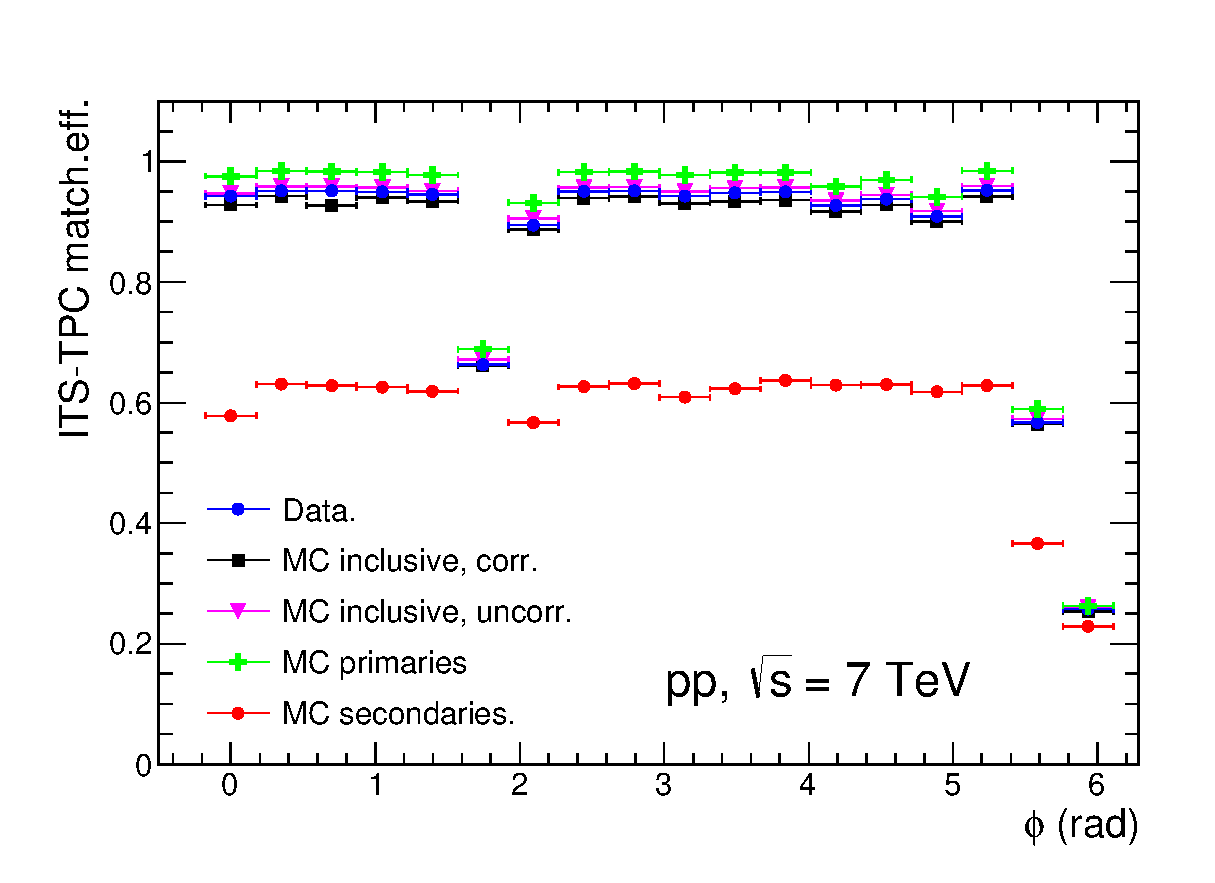
\includegraphics[width=.49\textwidth]{FigCap4/ITSTPCmatchEff_10bpass4_vsPhi.eps}
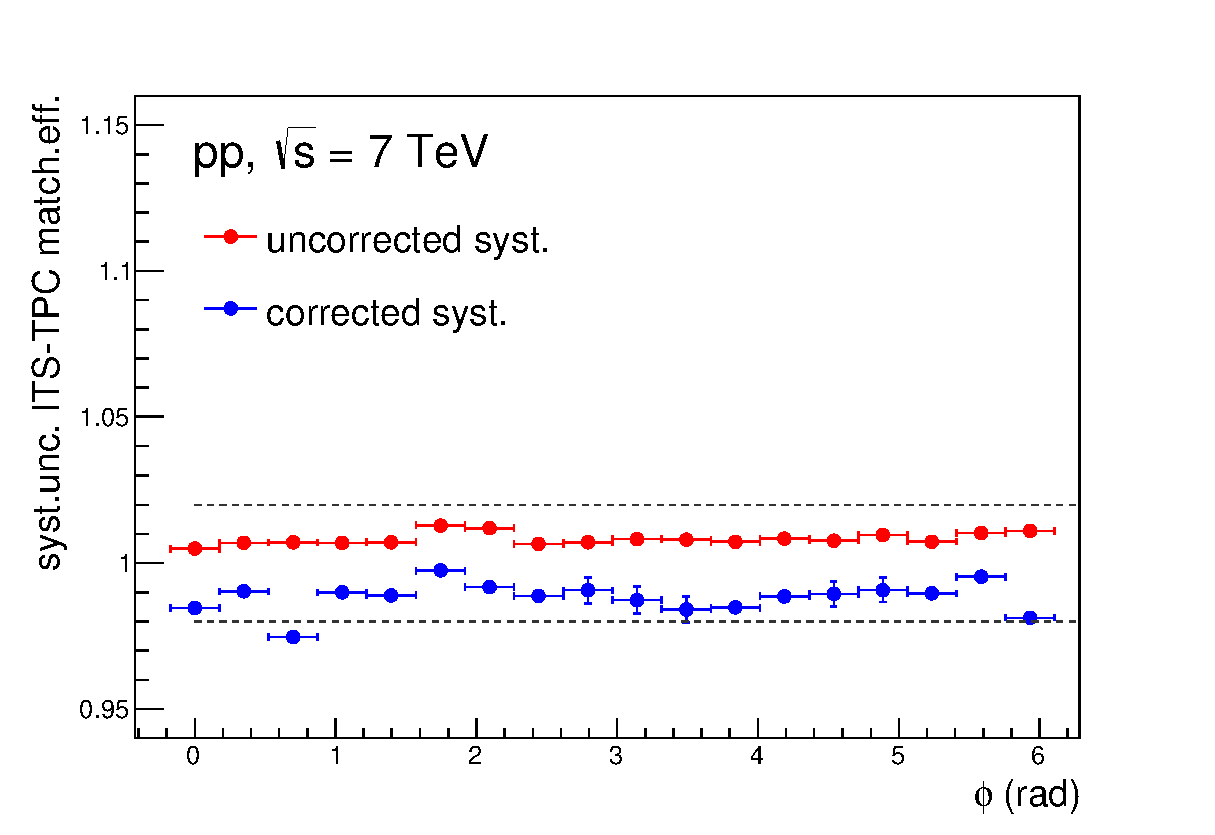
\includegraphics[width=.49\textwidth]{FigCap4/ITSTPCmatchEffSyst_10bpass4_vsPhi.eps}
\caption{Left: ITS-TPC matching efficiency as a function of $\phi$ for 2010 pp data taking at $\s = 7$ TeV. The $\pt$ of the tracks is \mbox{$0.5 < \pt < 14 \, \Gevc$}. The matching efficiency is shown for data (blu), for MC primary (green) and secondary (from strangeness decay and material interaction, in red) tracks, for inclusive MC tracks with (black) and without (magenta) data-driven correction. Right: ratio of ITS-TPC matching efficiencies in data and MC as a function of $\phi$ before (red) and after (blue) data-driven correction.}
\label{fig:CorrMatchEffVsPhi}
\end{center}
\end{figure}

\begin{figure}[!htb]
\begin{center}
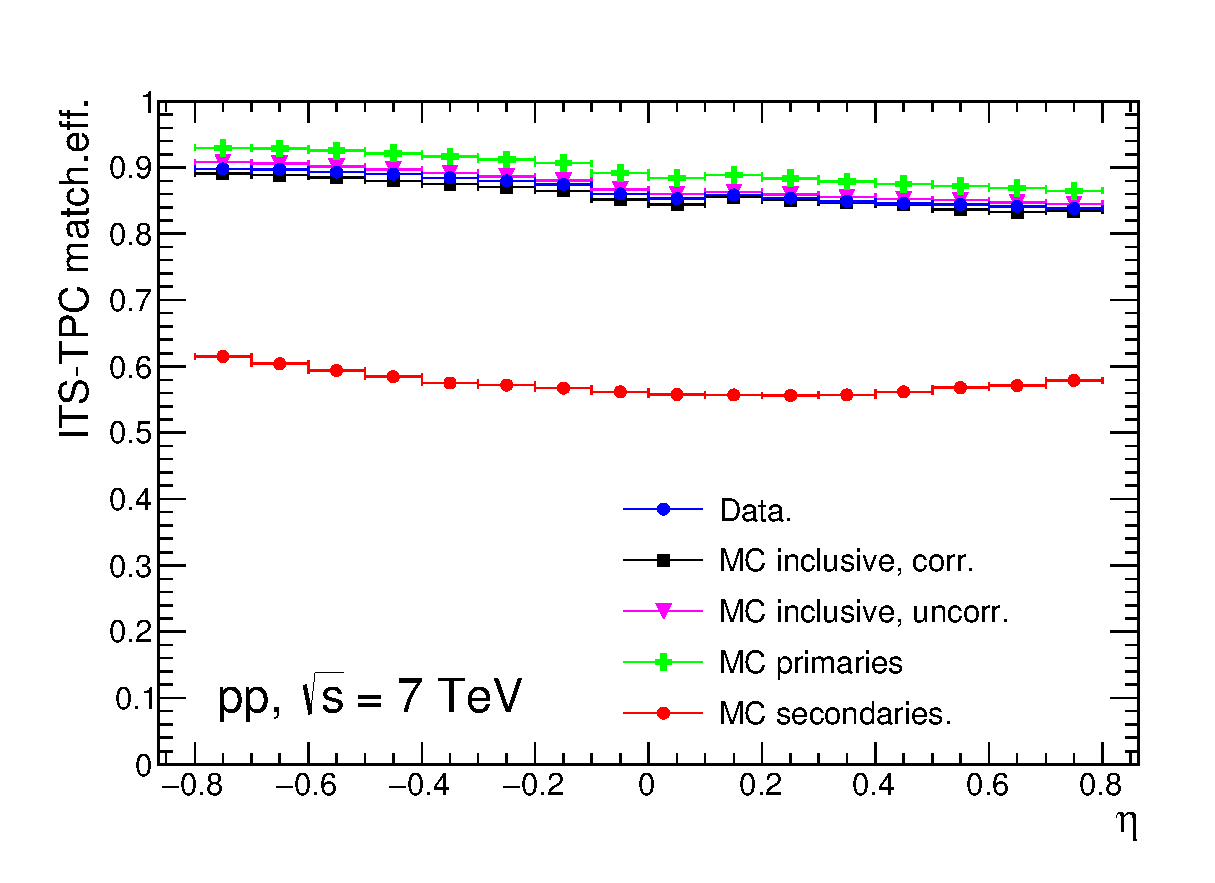
\includegraphics[width=.49\textwidth]{FigCap4/ITSTPCmatchEff_10bpass4_vsEta.eps}
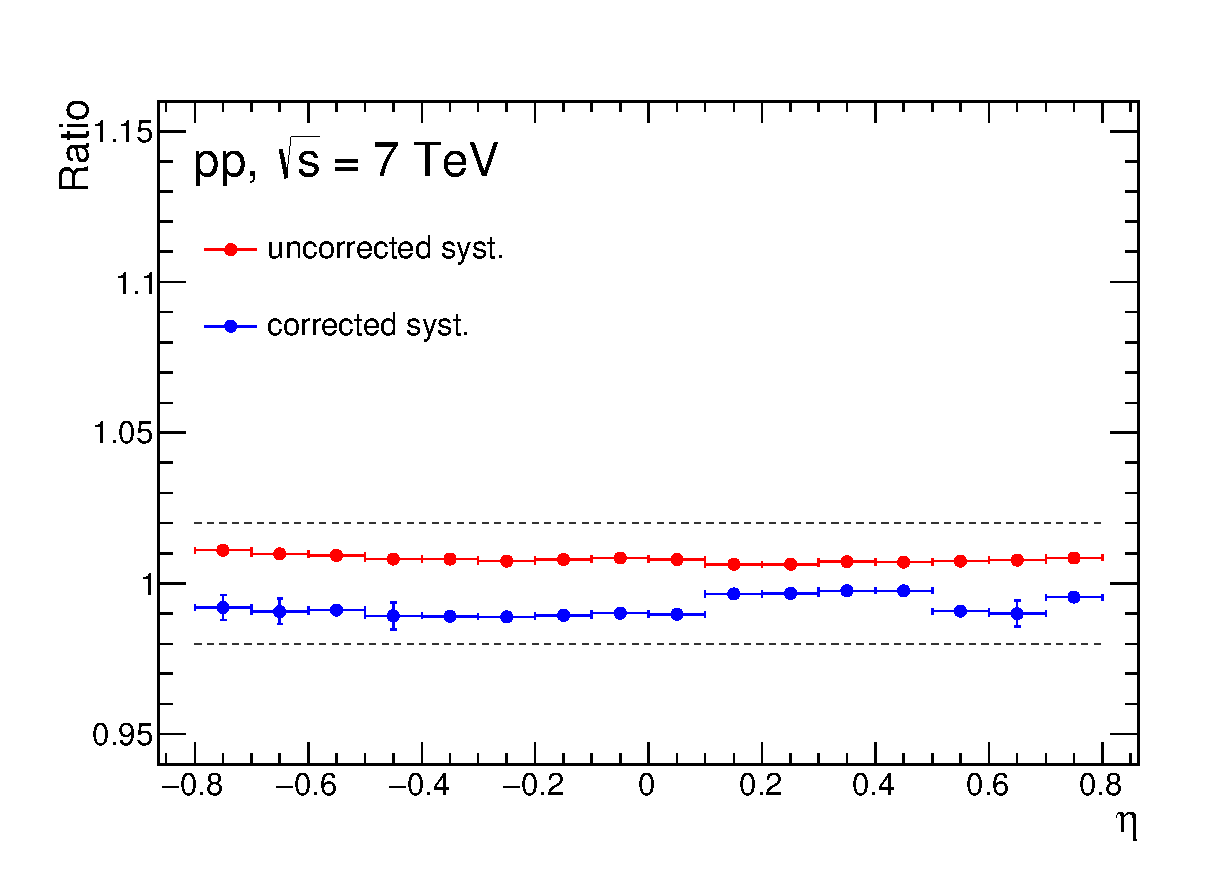
\includegraphics[width=.49\textwidth]{FigCap4/ITSTPCmatchEffSyst_10bpass4_vsEta.eps}
\caption{Left: ITS-TPC matching efficiency as a function of $\eta$ for 2010 pp data taking at $\s = 7$ TeV. The $\pt$ of the tracks is \mbox{$0.5 < \pt < 14 \, \Gevc$}. The matching efficiency is shown for data (blu), for MC primary (green) and secondary (from strangeness decay and material interaction, in red) tracks, for inclusive MC tracks with (black) and without (magenta) data-driven correction. Right: ratio of ITS-TPC matching efficiency in data and MC as a function of $\eta$ before (red) and after (blue) data-driven correction.}
\label{fig:CorrMatchEffVsEta}
\end{center}
\end{figure}


\begin{figure}[!htb]
\begin{center}
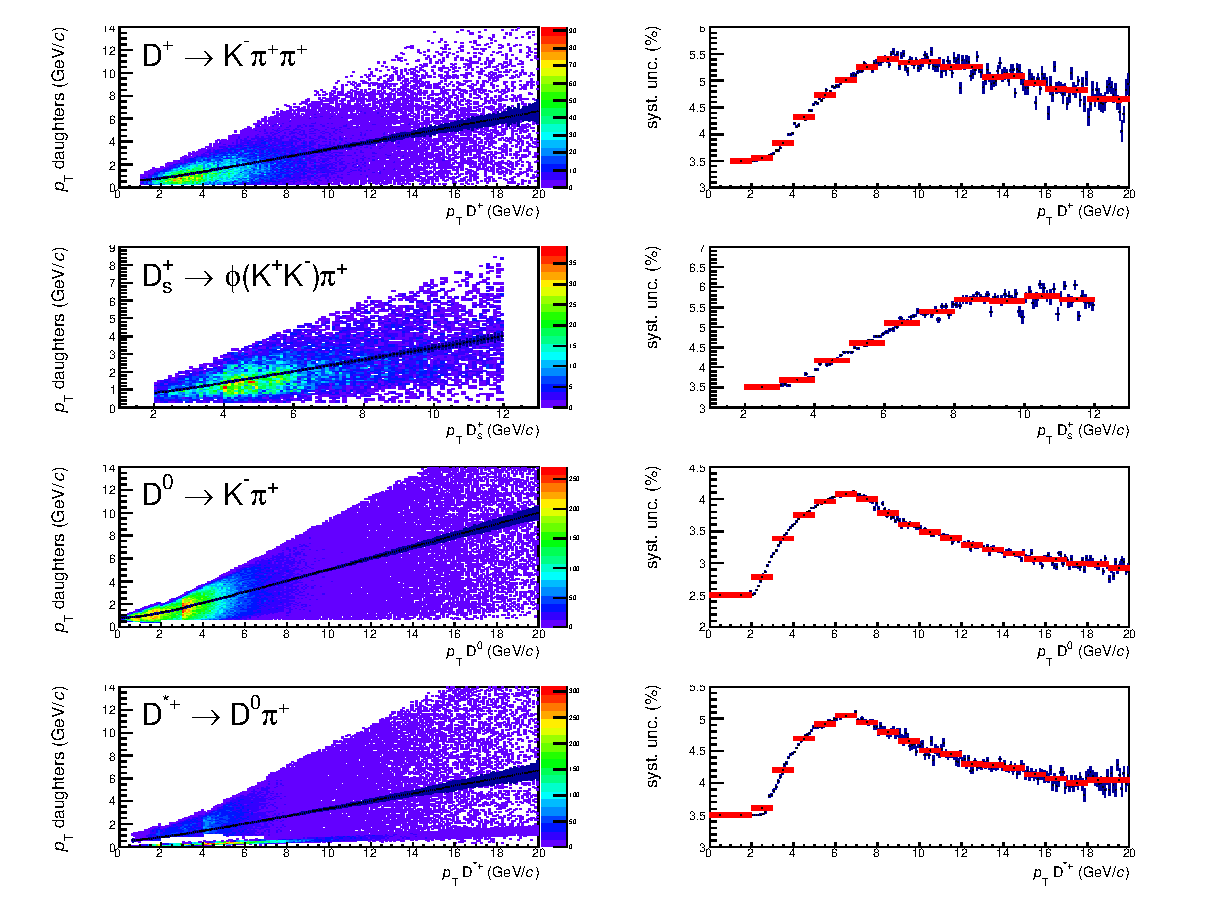
\includegraphics[width=1\textwidth]{FigCap4/FinalSystMEDmesons_ppPass4.eps}
\caption{Left: scatter plot of daughter $\pt$ versus $\Ds$-meson $\pt$. Right: final systematic uncertainties propagated at $\Ds$-meson level, after weighting for daughter kinematics, as a function of $\pt$.}
\label{fig:SysMatchEffDmeson}
\end{center}
\end{figure}

\subsection{B feed-down}
\label{sec:BfdSub}
The systematic uncertainty on the feed-down contribution, i.e. $\Ds$ mesons
originating from beauty-hadron decays in the raw yield, was estimated by varying the $\pt$-differential 
cross section of feed-down D mesons within the theoretical uncertainties
of the FONLL calculation. The procedure for the variation of the $b$-quark mass, 
of the perturbative scales and of the parton distribution functions is described 
in~\cite{Cacciari:2012ny}. The factorisation and renormalisation 
scales, $\mu_{\rm F}$ and $\mu_{\rm R}$, were made to vary independently 
in the ranges $0.5<\mu_{\rm F}/m_{\rm t}<2$, $0.5<\mu_{\rm R}/m_{\rm t}<2$, 
with the constraint $0.5<\mu_{\rm F}/\mu_{\rm R}<2$, 
where $m_{\rm t}=\sqrt{\pt^2+m_{\rm c}^2}$.
The mass of the c and b quarks were varied within $1.3<m_{\rm c}<1.7~\gev/c^2$ 
and $4.5<m_{\rm b}<5~\gev/c^2$, respectively.
The uncertainties on the fragmentation fractions of $b$ quarks into B mesons 
quoted in the PDG were kept into account. The uncertainty related to the B decay 
kinematics was neglected, after verifying that the difference resulting 
from using the PYTHIA~\cite{Sjostrand:2006za} decayer instead of 
EvtGen~\cite{Lange:2001uf} is negligible 
with respect to the FONLL B-meson cross-section uncertainty.
Previous D-meson analyses in 
ALICE~\cite{ALICE:2011aa,Adam:2016ich,Adam:2015jda} 
used to compare two different methods to correct for the beauty feed-down component 
and include their difference in the systematic uncertainty. 
The first method, used to give the central value for $f_{\rm prompt}$, 
is the one presented in Eq.~\ref{eq:fpr} and needs as inputs the measured $\Dspm$ raw yields, the FONLL predictions
of B-meson cross-sections and the selection efficiency for feed-down 
D mesons. The alternative method takes as inputs FONLL predictions for both 
feed-down and prompt D mesons and their respective Monte Carlo efficiencies, 
as follows:
\begin{equation}
f^\prime_{\rm prompt} = \left( 	1 + 	\frac{({\rm Acc}\times\epsilon)_{{\rm feed-down}}}{({\rm Acc}\times\epsilon)_{{\rm prompt}}}	\cdot
		 \frac{ \left(\frac{{\rm d}^2 \sigma}{{\rm d}y \, {\rm d} \pt } \right)^{{\sf FONLL}}_{{\rm feed-down}} }{ \left(\frac{{\rm d}^2 \sigma}{{\rm d}y \, {\rm d} \pt } \right)^{{\sf FONLL}}_{ {\rm prompt} } } 
\right)^{-1} \, .
\label{eq:fc}
\end{equation}
The usage of this alternative approach has been reconsidered after a
review of currently available measurements of beauty and 
charmed meson cross-sections at the LHC was carried out. The measurements 
were compared to FONLL predictions for heavy-flavoured hadrons 
for the specific center-of-mass energy and rapidity interval.
In Fig.~\ref{fig:Bmesons}, the B$^{+}$-, B$^{0}$-, B$^0_{\rm s}$-meson and 
$\Lambda_{\rm b}$-baryon cross sections measured by CMS in pp collisions 
at $\s = $ 7 TeV~\cite{Khachatryan:2011mk,Chatrchyan:2011pw,Chatrchyan:2011vh,Chatrchyan:2012xg},
in the rapidity interval $|y| <$ 2.4, are compared to FONLL predictions. 
The latter were rescaled for the fragmentation fractions of $b$ quark into 
$b$ hadrons from PDG~\cite{Patrignani:2016xqp}, which provides the production 
fractions of $b$ hadrons in hadronic Z decays.
The measurements lay within FONLL uncertainty bands in the case 
of non-strange B mesons. A worse agreement for FONLL is found to B$^0_{\rm s}$-meson
and $\Lambda_{\rm b}$-baryon cross sections.
In Fig.~\ref{fig:LHCbBmesons}, measurements of B$^{+}$-, B$^0_{\rm s}$-meson
and $\Lambda_{\rm b}$-baryon cross sections from
LHCb in pp collisions at $\s =$ 7 TeV at forward rapidity 
\mbox{2.0 $< y <$ 4.5} are shown~\cite{Aaij:2013noa,Aaij:2015fea}.
FONLL predictions were scaled by the fragmentation fraction values 
of $b$ quarks into $b$ hadrons measured by LHCb in the rapidity interval 
2.0 $< y <$ 4.5~\cite{Aaij:2011jp}. The LHCb measurements in pp collisions indicate an 
enhancement of baryon production from $b$-quark fragmentation at forward rapidity with respect to 
the value quoted by the PDG~\cite{Patrignani:2016xqp}. The values from LHCb are in agreement with the measurements
of the $b$-quark fragmentation fraction in p$\bar{\rm p}$ collisions at Tevatron reviewed in~\cite{Patrignani:2016xqp}.
In Tab.~\ref{tab:fragFrac}, the fragmentation fractions of beauty quarks at Z resonance and
in p$\bar{\rm p}$ collisions are summarised:\\
\begin{table}[!h]
\centering
\begin{tabular}{l|ccc}
 \hline 
\hline
$b$ hadron & fraction at Z $[\%]$  & fraction at p$\bar{\rm p}$ \\
\hline 
${\rm B}^{+}$, ${\rm B}^{0}$    &     40.7 $\pm$ 0.7   & 34.4 $\pm$ 2.1 \\
${\rm B}_{s}$                 &     10.0 $\pm$ 0.8   & 11.5 $\pm$ 1.3 \\
$b$ baryons          &       8.5 $\pm$ 1.1   & 19.7 $\pm$ 4.6 \\
 \hline 
\hline
\end{tabular}
\caption{Fragmentation fractions of $b$ quarks into weakly-decaying $b$-hadron species in Z$ \rightarrow b\bar{b}$ decay, in p$\bar{\rm p}$ collisions at $\s = 1.96$ TeV~\cite{Patrignani:2016xqp}.}
\label{tab:fragFrac}
\end{table}




In the top left panel of Fig.~\ref{fig:LHCbBmesons} the 
comparison between LHCb B$^{+}$-meson cross section and the FONLL
 calculations shows a good agreement. Also the $\Lambda_{\rm b}$-baryon cross section (top-right panel)
 is well described by FONLL, provided that the value of $f(b\rightarrow \Lambda_{\rm b})$
measured in pp or p$\bar{\rm p}$ collisions is used. This supports the evidence for non-universality of
hadronisation fractions in the two different environment of pp (p$\bar{\rm p}$) collisions
and in Z decay. 
\begin{figure}[!htbp]
\begin{center}
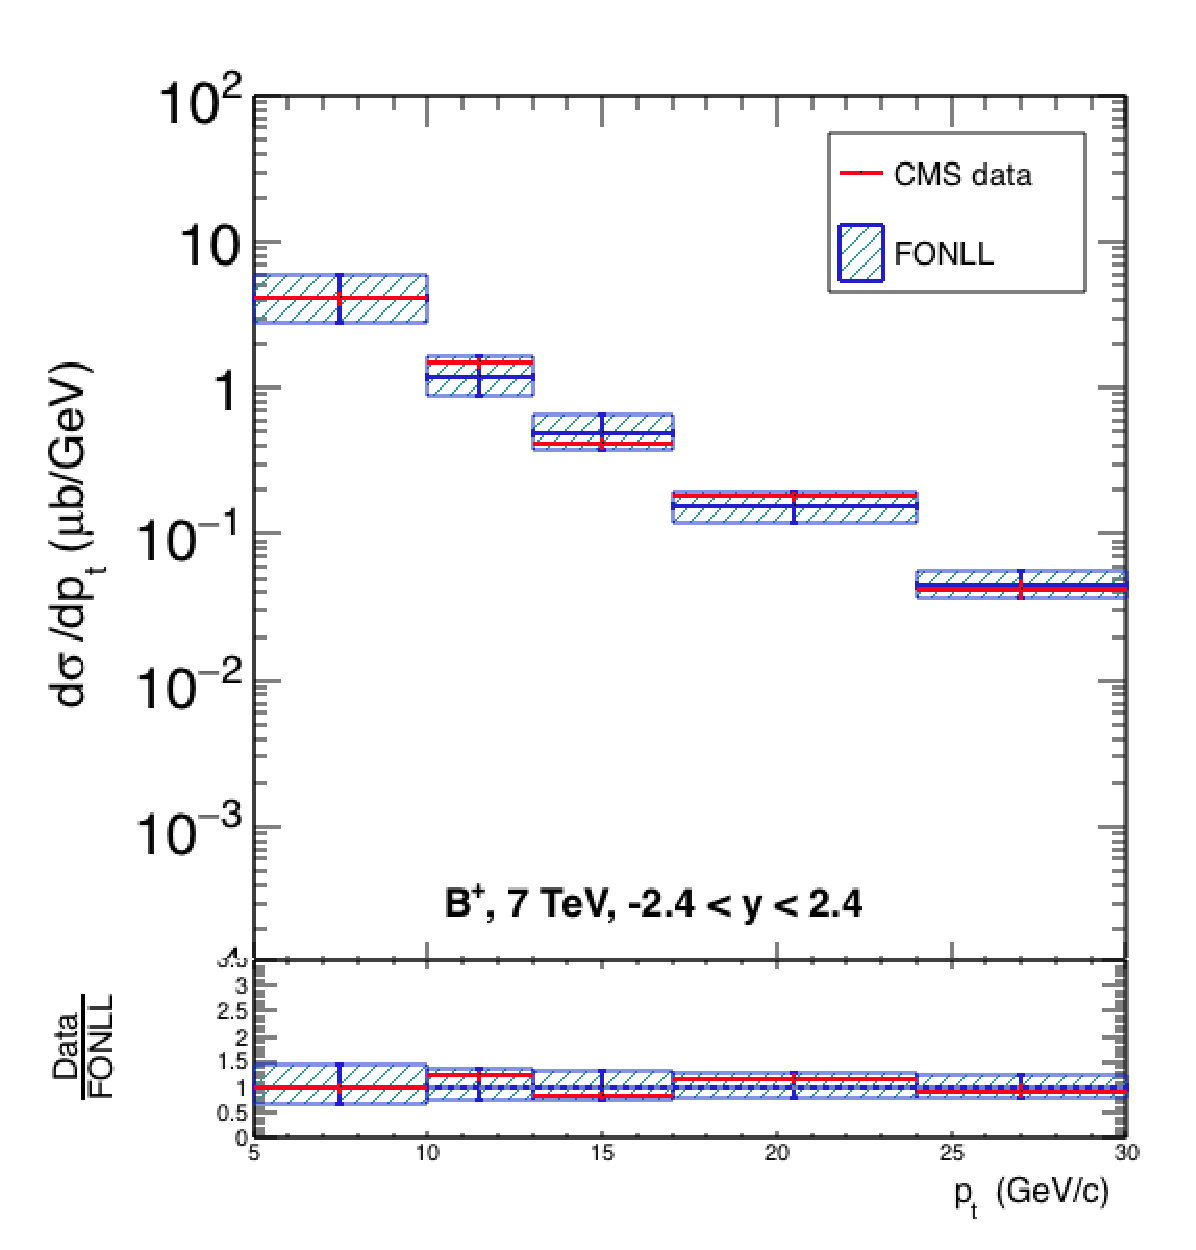
\includegraphics[width=.45\textwidth]{FigCap4/Bplus_7TeV_y_24_24.eps}
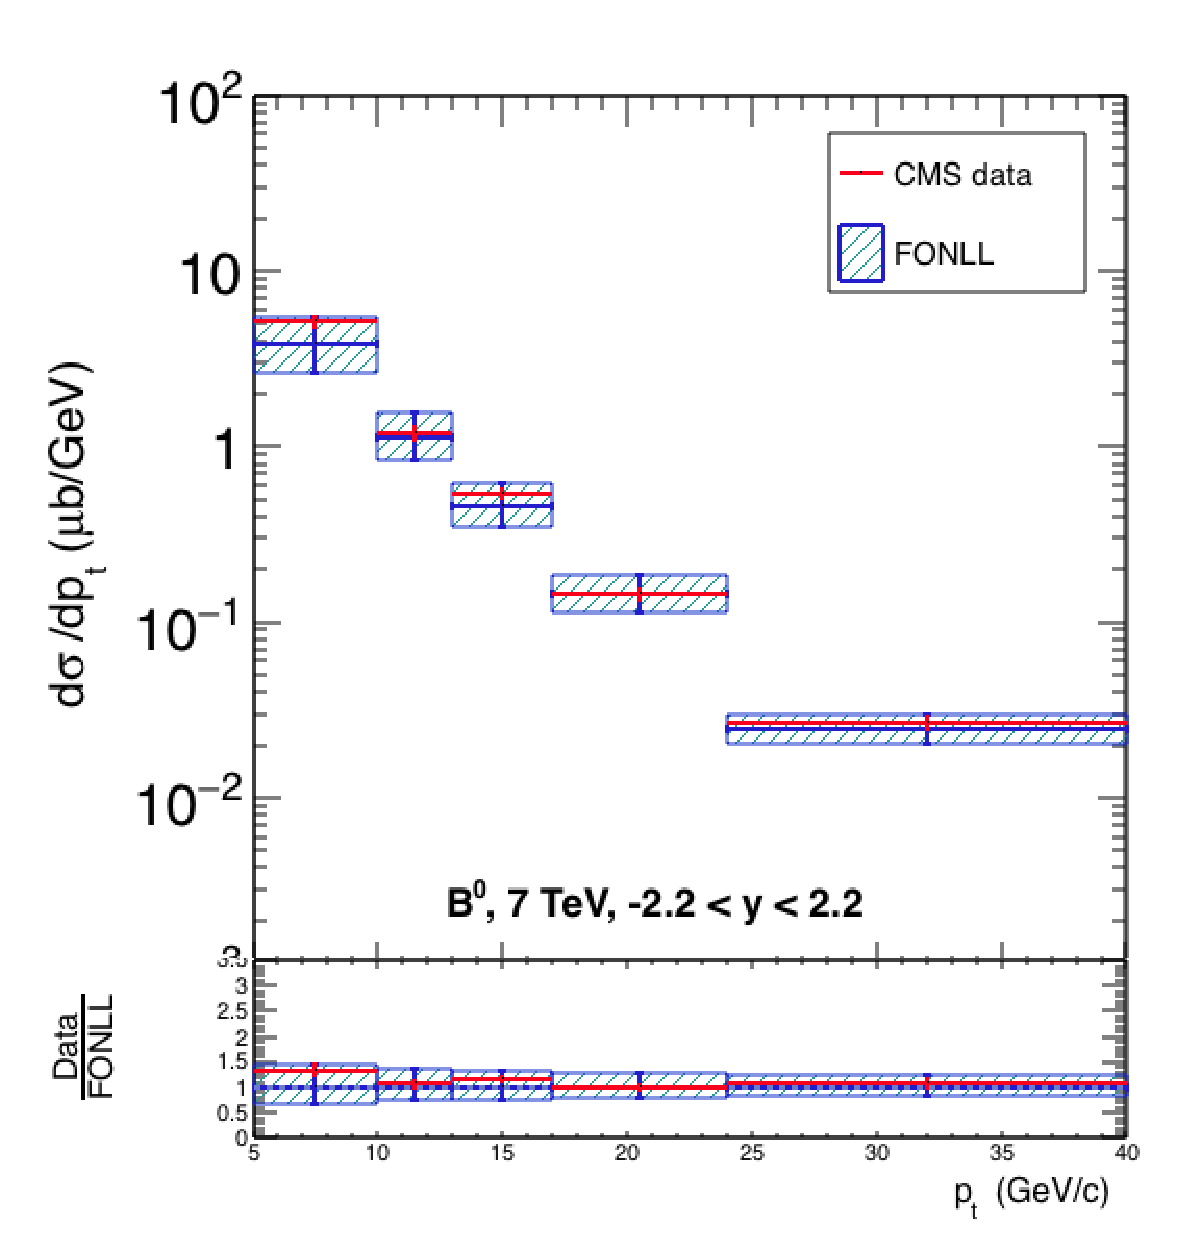
\includegraphics[width=.45\textwidth]{FigCap4/Bzero_7TeV_y_22_22.eps}
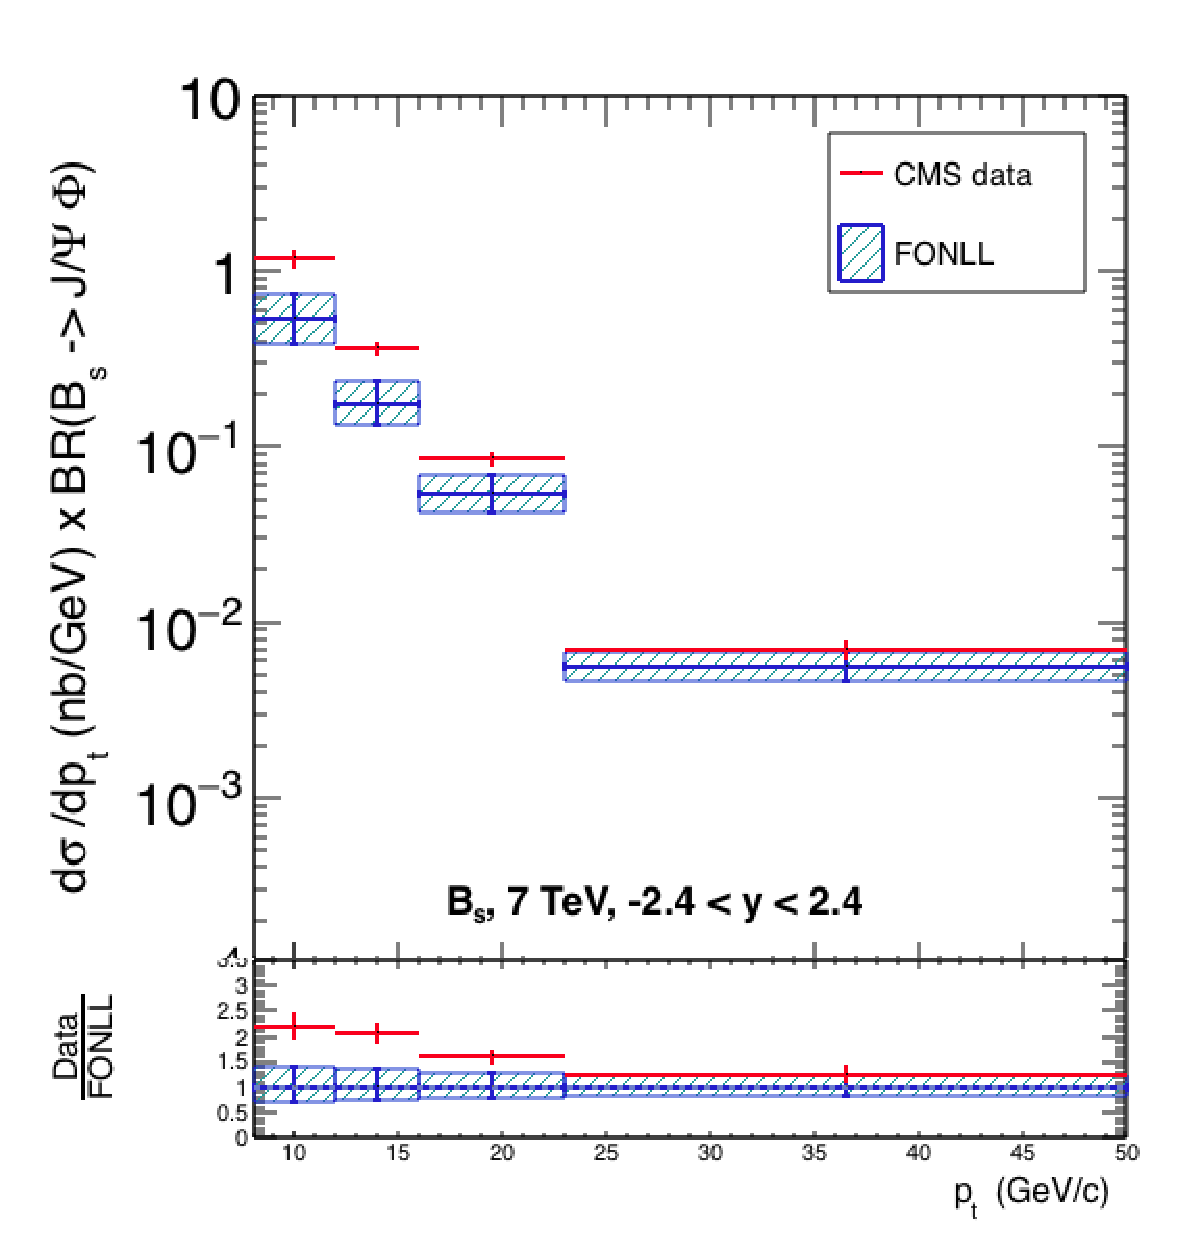
\includegraphics[width=.45\textwidth]{FigCap4/Bs_7TeV_y_24_24.eps}
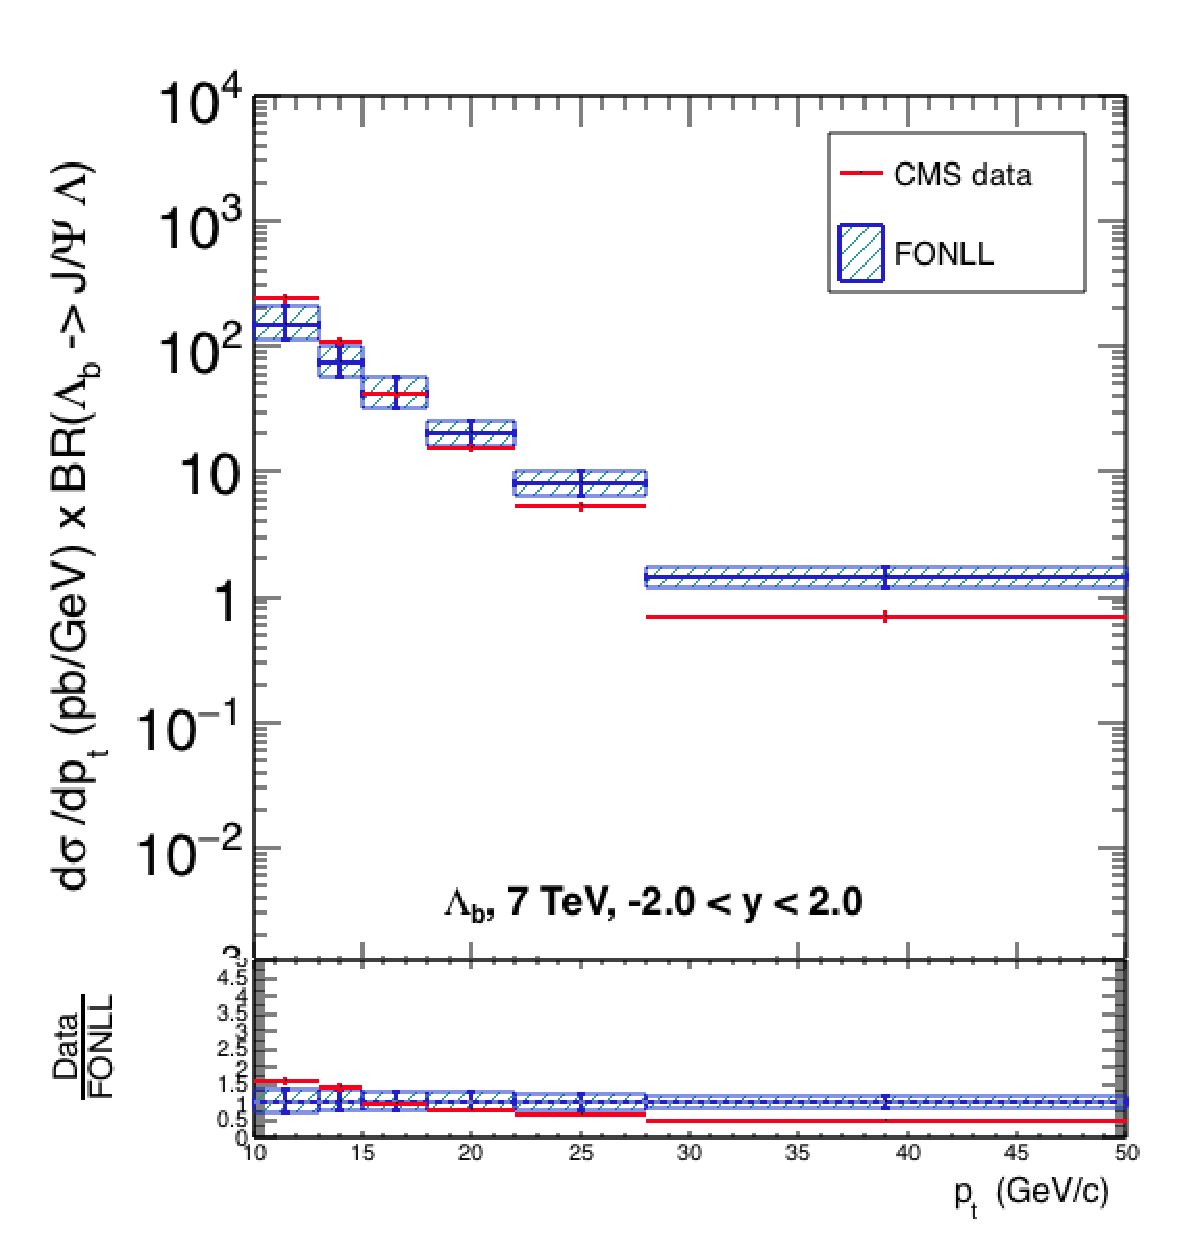
\includegraphics[width=.45\textwidth]{FigCap4/Lambdab_7TeV_y_20_20.eps}
\caption{B$^{+}$-, B$^{0}$-, B$_{\rm s}$-meson and $\Lambda_{\rm b}$-baryon differential cross-sections (red points) as a function of $\pt$ measured by CMS in pp collisions at $\s =$ 7 TeV at mid-rapidity~\cite{Khachatryan:2011mk,Chatrchyan:2011pw,Chatrchyan:2011vh,Chatrchyan:2012xg} compared to FONLL predictions~\cite{Cacciari:1998it, Cacciari:2001td} at the same energy (blue boxes). }
\label{fig:Bmesons}
\end{center}
\end{figure}
\begin{figure}[!htbp]
\begin{center}
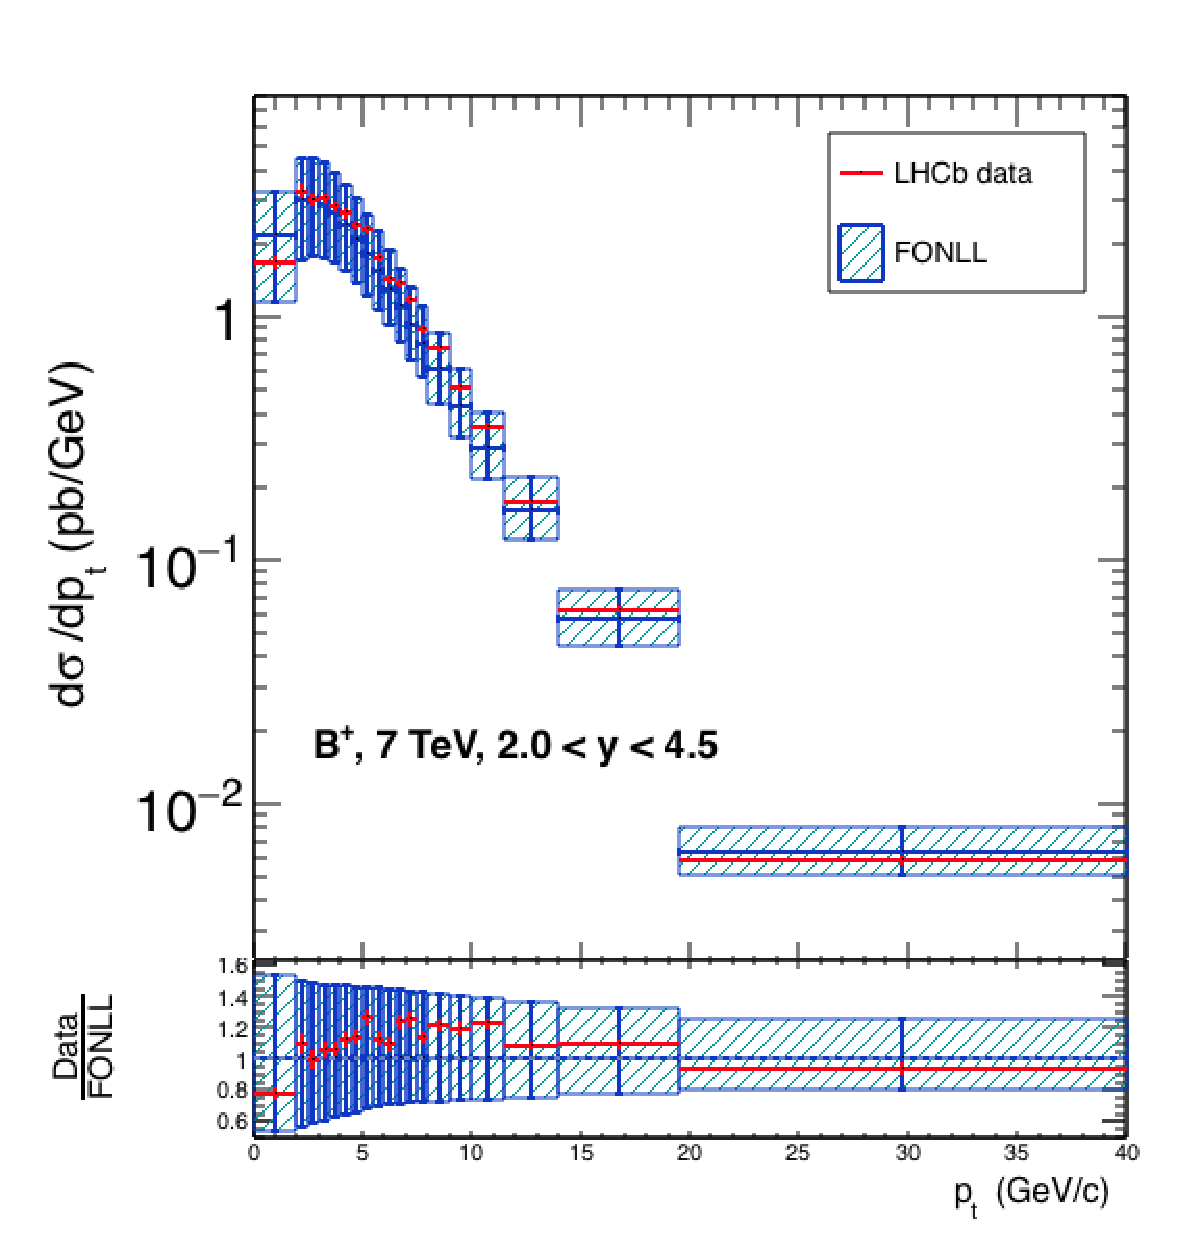
\includegraphics[width=.45\textwidth]{FigCap4/Bplus_7TeV_y_20_45_FF35.eps}
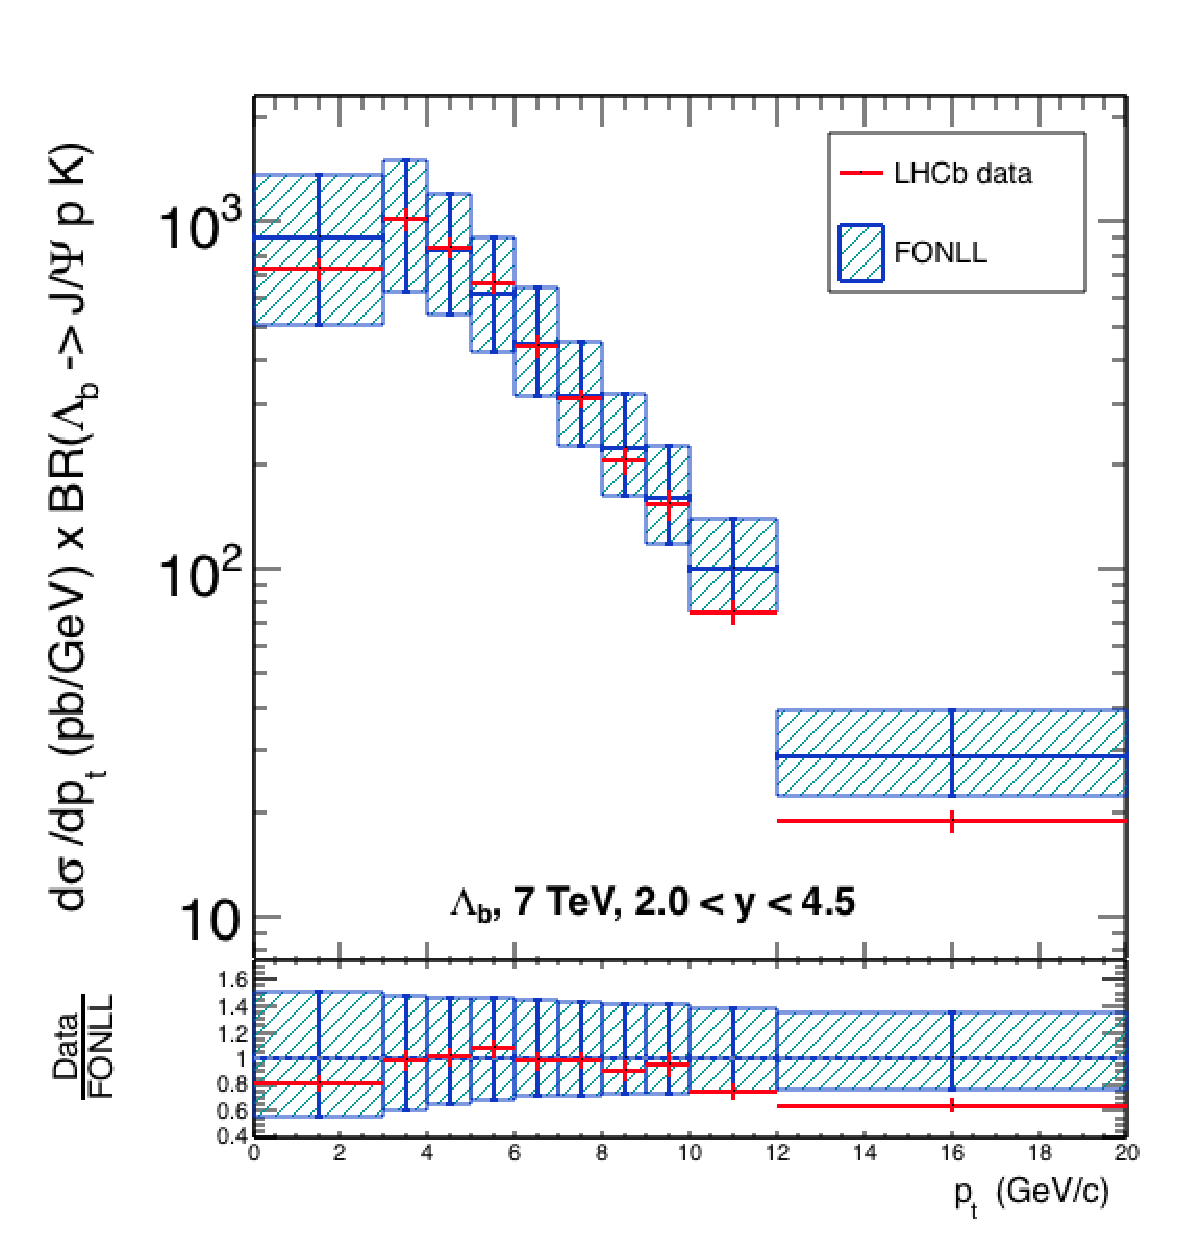
\includegraphics[width=.45\textwidth]{FigCap4/Lambdab_7TeV_y_20_45_FF21_BR6.eps}
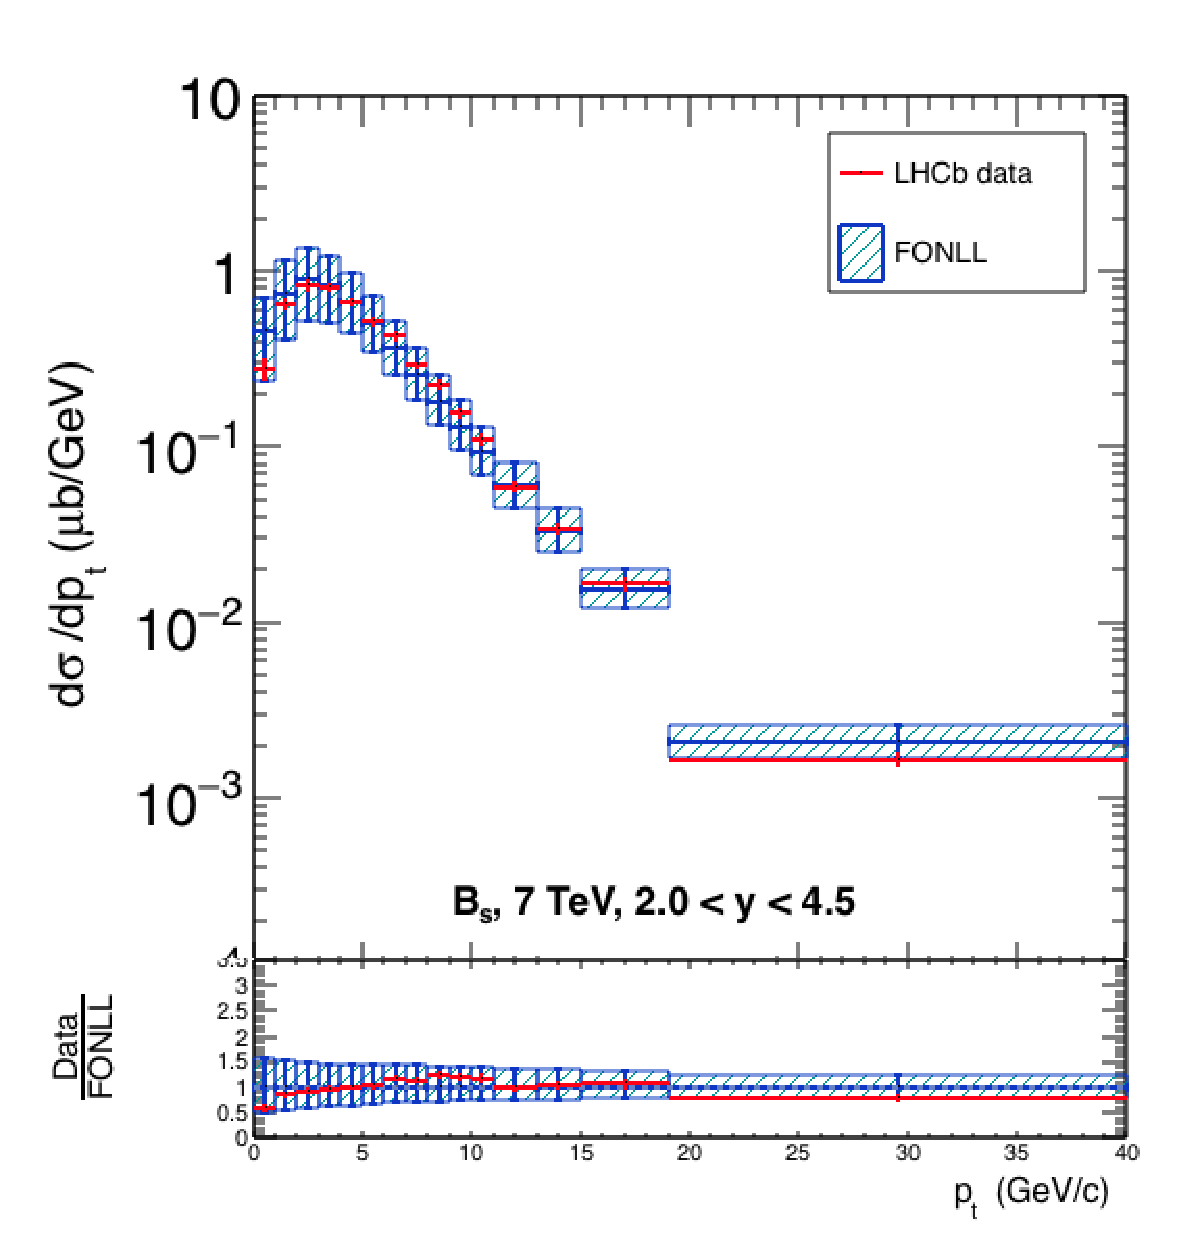
\includegraphics[width=.45\textwidth]{FigCap4/Bs_7TeV_y_20_45.eps}
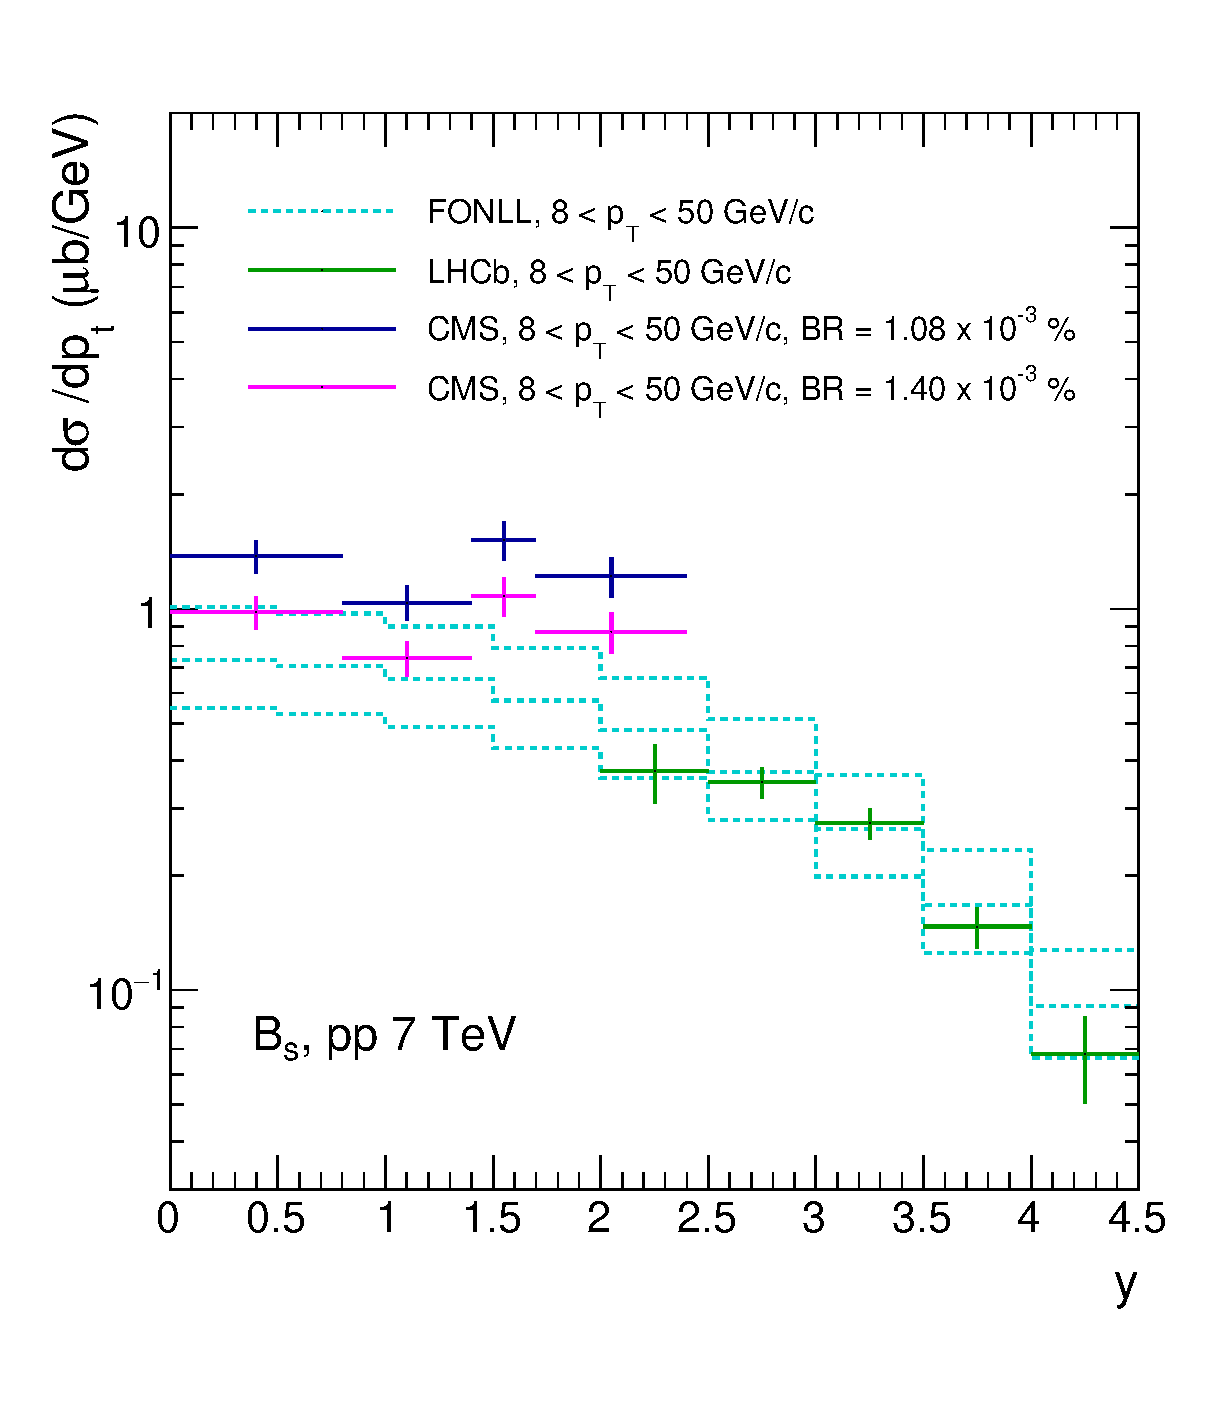
\includegraphics[width=.4\textwidth]{FigCap4/FONLL_CMSVsLHC_2.eps}
\caption{B$^{+}$, $\Lambda_{\rm b}$ and B$^0_{\rm s}$ differential cross-sections (red points) measured by LHCb in pp collisions at $\s =$ 7 TeV at \mbox{2 $< y <$ 4.5} compared to FONLL predictions at the same energy (blue boxes)~\cite{Aaij:2013noa,Aaij:2015fea}.
In the bottom right panel, B$^0_{\rm s}$-meson differential cross-section as a function of $y$ from LHCb is compared to same measurements from CMS at mid-rapidity (8 $< p_{\rm T} <$ 50 GeV/$c$) and to FONLL predictions~\cite{Cacciari:1998it, Cacciari:2001td} in the full rapidity range. }
\label{fig:LHCbBmesons}
\end{center}
\end{figure}
\begin{figure}[!htbp]
\begin{center}
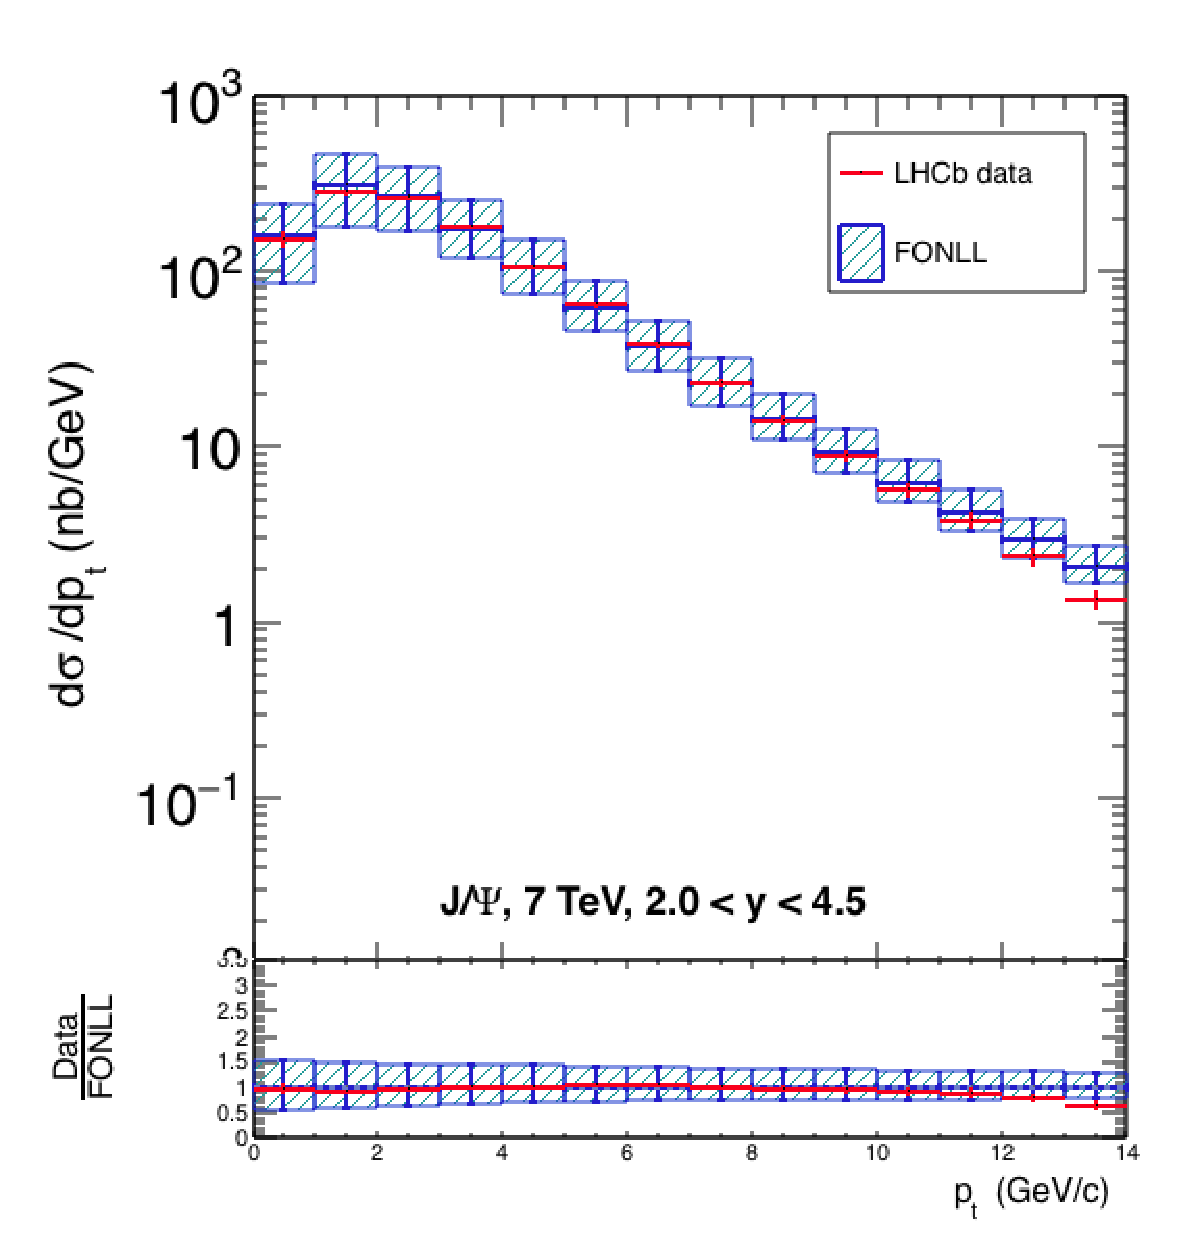
\includegraphics[width=.45\textwidth]{FigCap4/Jpsi_7TeV_y_20_45.eps}
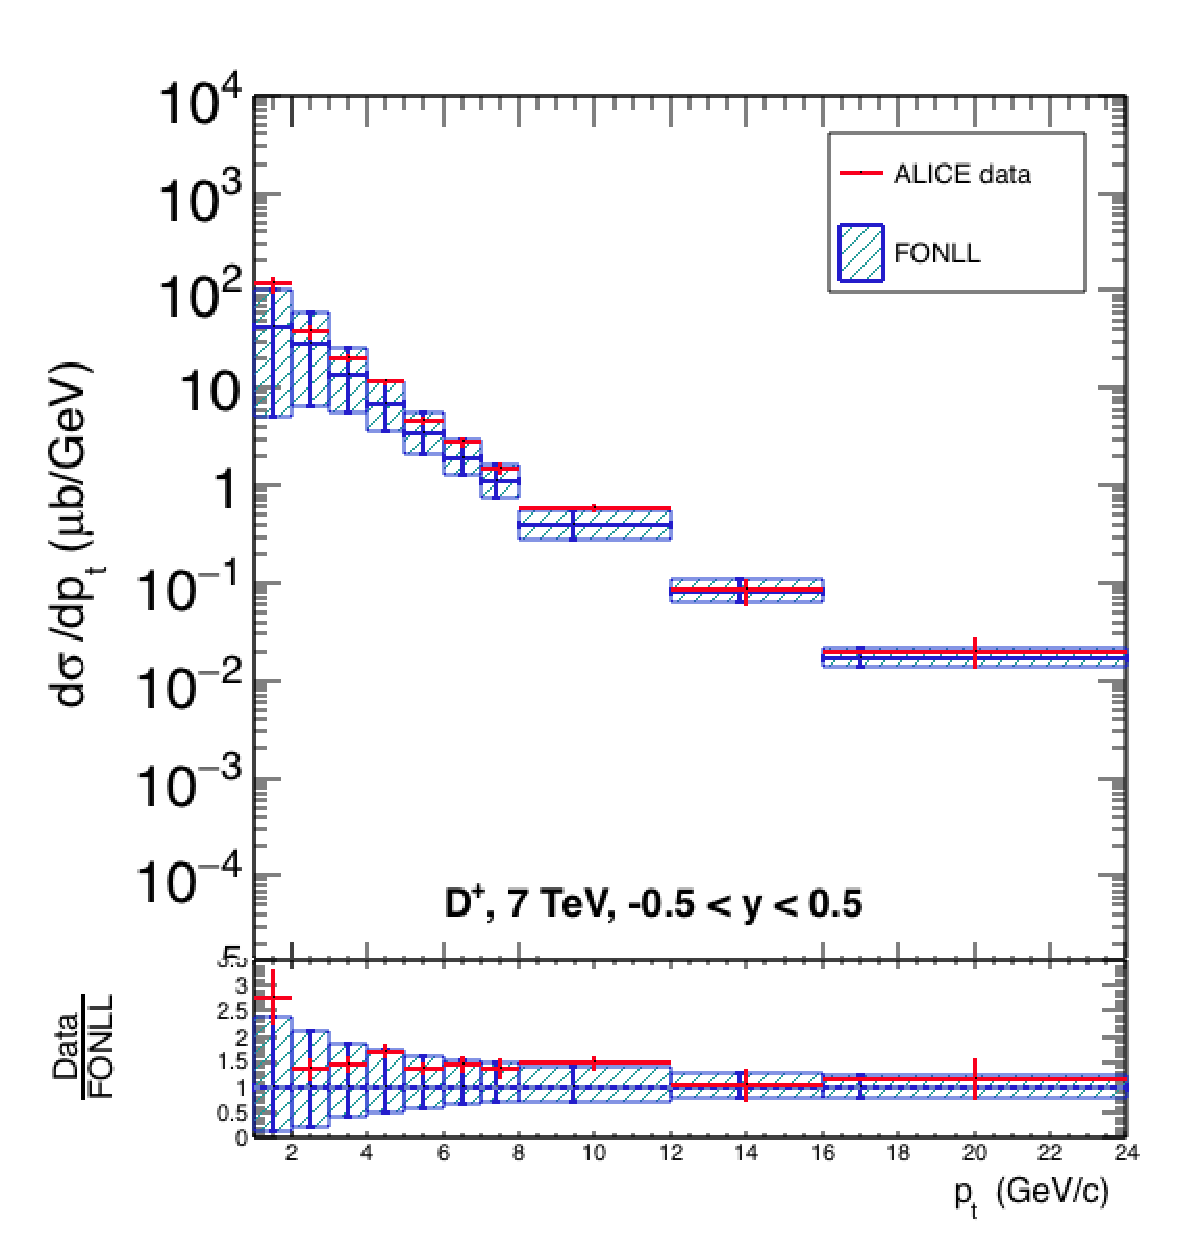
\includegraphics[width=.45\textwidth]{FigCap4/Dplus_7TeV_y_05_05.eps}
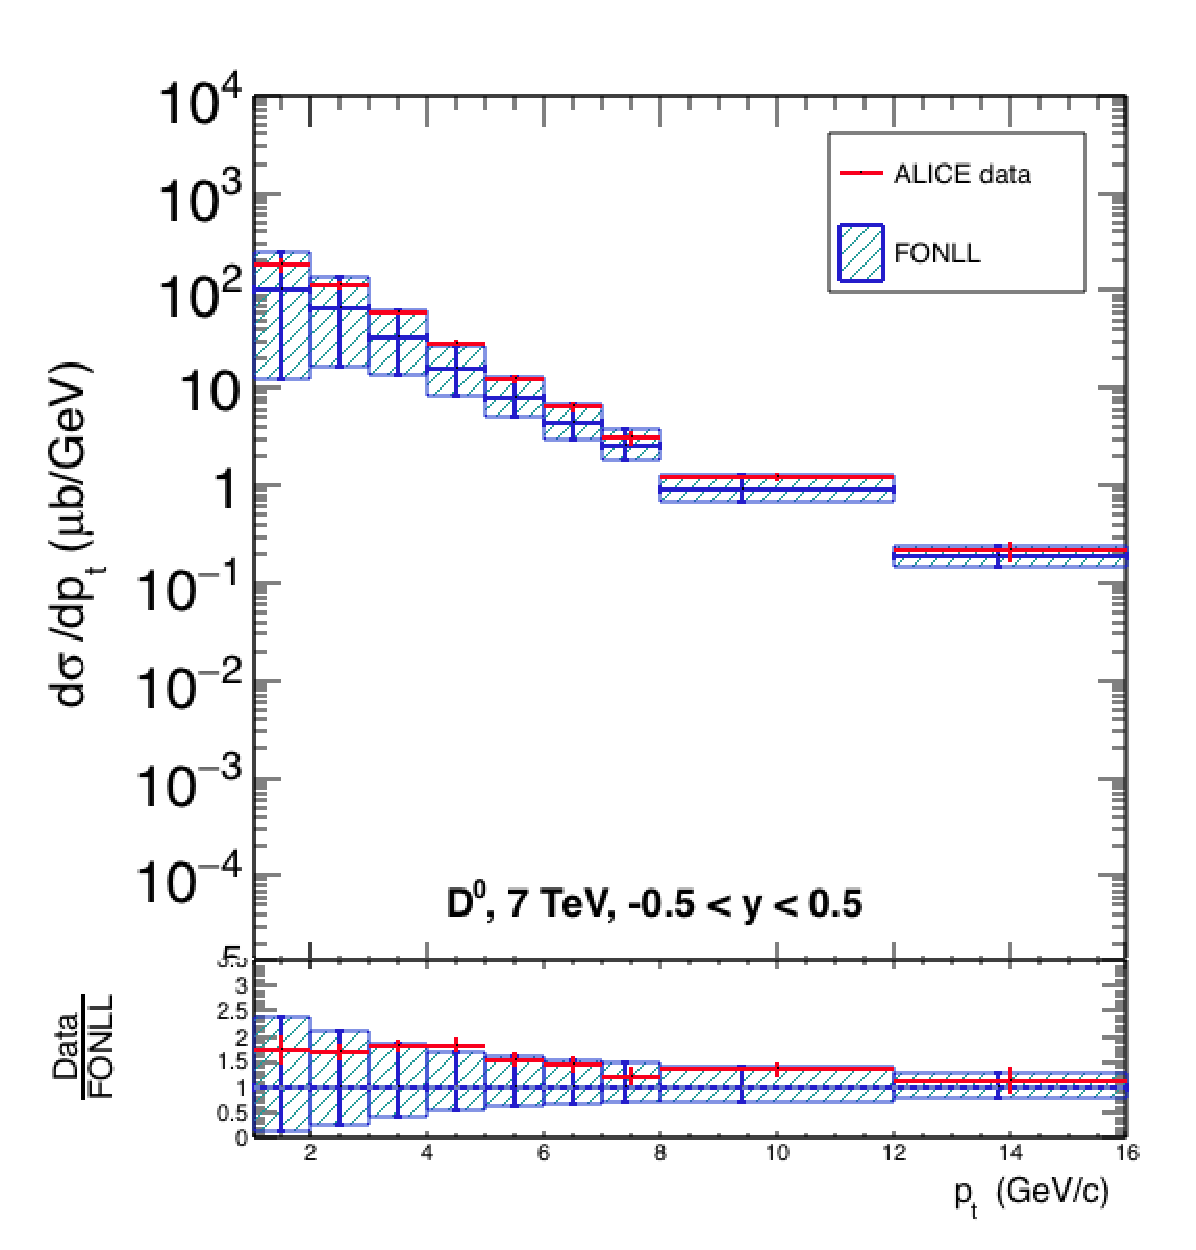
\includegraphics[width=.45\textwidth]{FigCap4/Dzero_7TeV_y_05_05.eps}
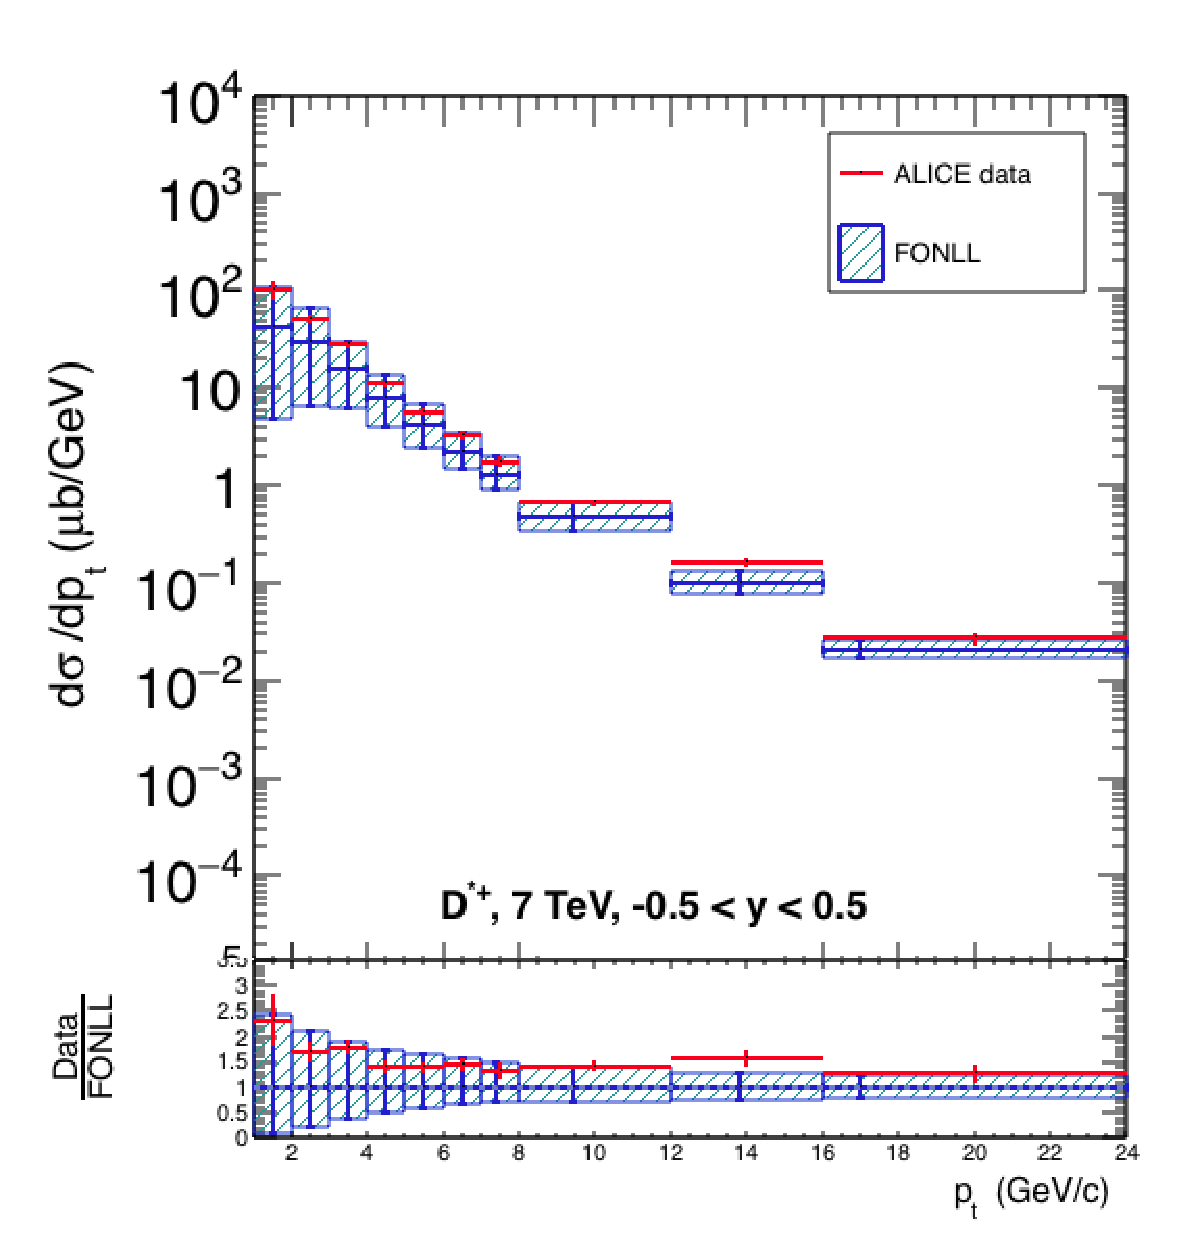
\includegraphics[width=.45\textwidth]{FigCap4/Dstar_7TeV_y_05_05.eps}
\caption{J/$\psi$ from $b$-hadron decays (from LHCb, \mbox{2 $< y <$ 4.5}~\cite{Aaij:2011jh}), D$^{+}$, D$^{0}$ and $\Dstar$-meson (from ALICE, mid-rapidity~\cite{ALICE:2011aa}) differential cross-sections (red points) as a function of $\pt$ in pp collisions at $\s = $ 7 TeV compared to FONLL predictions~\cite{Cacciari:1998it, Cacciari:2001td} at the same energy (blue boxes). }
\label{fig:Dmesons}
\end{center}
\end{figure}
A better agreement is found for 
LHCb B$^0_{\rm s}$-meson cross-section with FONLL calculations (bottom left panel), measured in a wider 
$p_{T}$ range than CMS. The CMS and LHCb B$^0_{\rm s}$-meson cross-sections in 
8 $< p_{\rm T} <$ 50 GeV/$c$ are shown in 
the bottom right panel as a function of $y$, together with FONLL predictions in the 
two different rapidity intervals. For the CMS data, two cases are 
reported, one obtained using the 2015 PDG~\cite{Agashe:2014kda} value for 
BR(B$_{\rm s} \rightarrow J/{\rm \psi} ~\phi$) = (1.40 $\pm$ 0.04)$\times 10^{-3}$,
the other obtained using the 2010 PDG~\cite{Nakamura:2010zzi} value BR = (1.08 $\pm$ 0.09)$\times 10^{-3}$, 
referenced in the CMS paper. The agreement of FONLL to the measurements is good
at forward rapidity and also at mid-rapidity when the updated value of BR(B$_{\rm s} \rightarrow J/{\rm \psi} ~\phi$) is used.
In Fig.~\ref{fig:Dmesons} the cross-section 
of $J/\psi$-meson from beauty-hadron decays in pp collisions at 
$\s = $ 7 TeV measured by LHCb~\cite{Aaij:2011jh} and 
the D$^{+}$-, D$^{0}$-, D$^{*+}$-meson cross-sections in pp collisions at $\s = $ 7 TeV by ALICE~\cite{ALICE:2011aa}
are presented. For $J/\psi$ mesons from beauty decays, FONLL provides a good description of 
the data (note that this holds also for data at $\s =$ 8 TeV~\cite{Aaij:2013yaa}). 
The D-meson results show that the measurements 
systematically lay on the upper edge of FONLL uncertainty 
band, thus charm production being underestimated by the FONLL
calculation with the central values of charm mass ($m_c = 1.5 \, \Gevc$) and
of factorisation and renormalisation scales.\\
\begin{figure}[!h]
\begin{center}
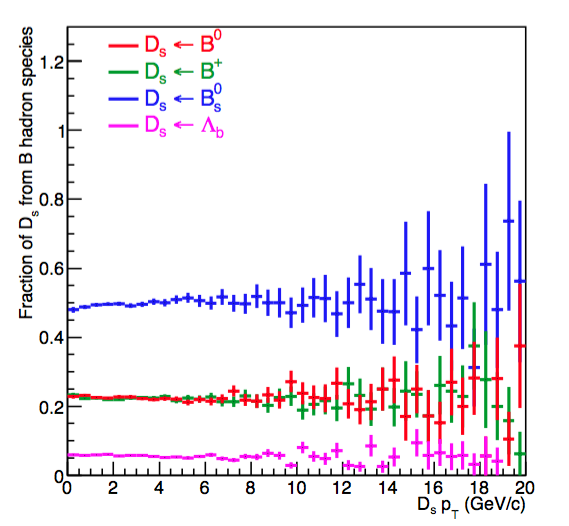
\includegraphics[width=0.49\textwidth]{FigCap4/DsParents.png}
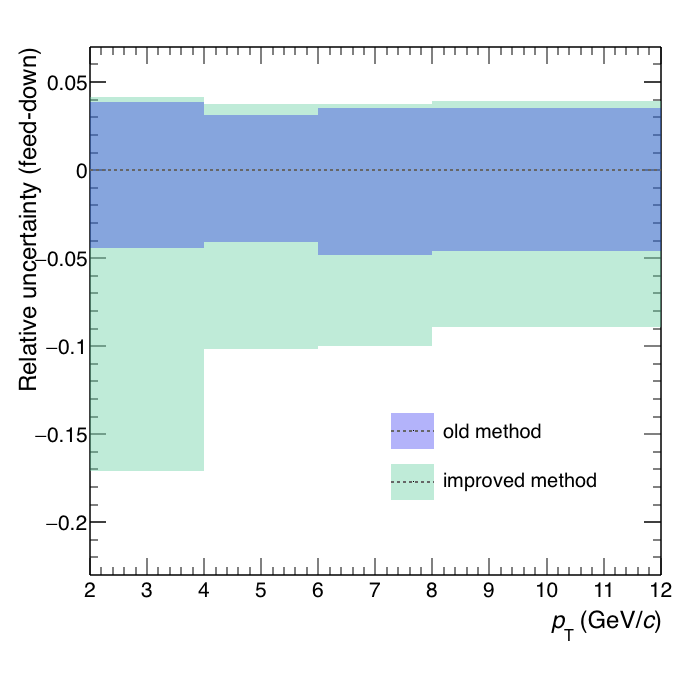
\includegraphics[width=0.49\textwidth]{FigCap4/comparisonFDerr_pass2_pass4.png}
\caption{Left: fraction of $\Ds$ originating from decays of different species of beauty hadrons. Right: comparison of systematic uncertainties on beauty feed-down component subtraction with the old and the new procedure.}
\label{fig:DsParentsAndFDunc}
\end{center}
\end{figure}
Considering that:
\begin{itemize}
\item FONLL provides a good description of B$^{+}$- and B$^{0}$-meson 
cross-sections at $\s =$ 7 TeV at both mid- and forward rapidity and of 
the cross-section of $J/{\rm \psi}$ from beauty-hadron decays at forward rapidity at  $\s =$ 7, 8 TeV;
\item FONLL provides a good description also for the 
B$^0_{\rm s}$-meson cross-section at forward rapidity where data are available in a wider $\pt$ range 
than at mid-rapidity. FONLL also describes 
$\Lambda_{\rm b}$-baryon cross-section, provided 
the usage of the $f(b\rightarrow \Lambda_{\rm b})$ measured in pp collisions;
\end{itemize}
the calculation of $f_{\rm prompt}$ with the method in Eq.~\ref{eq:fpr} is then fully justified.
Indeed, as Fig.~\ref{fig:DsParentsAndFDunc} (left) shows, around half of B feed-down 
$\Ds$ originates from B$^0$- and B$^+$-meson decays 
and half from B$^0_{\rm s}$-meson decays, which are all described
by FONLL calculations. The sum of the contributions to the $\Ds$ yield shown in Fig.~\ref{fig:DsParentsAndFDunc} (left) is unity.
The method in Eq.~\ref{eq:fc}, instead, would suffer from the 
fact that FONLL underestimates charm production at LHC energies. 
It is reasonable to conclude that, on the basis of the current 
measurements, Eq.~\ref{eq:fc} could introduce a bias if 
used to correct for the beauty feed-down component, thus artificially enhancing 
the systematic uncertainty. In Fig.~\ref{fig:DsParentsAndFDunc} (right) the comparison of the 
relative (low and high) systematic uncertainties on the $\Ds$ cross-section, 
due to the beauty feed-down subtraction, show that the lower uncertainties are reduced by a factor 2-3, 
depending on $\pt$, with the improved procedure with respect to the old one.
The low uncertainty bars result the most affected by the reduction since the estimate of the prompt
fraction with Eq.~\ref{eq:fc} is systematically lower than that with Eq.~\ref{eq:fpr},
because FONLL calculations underestimate charm production at LHC.

\subsection{Generated $\pt$ shape}
\label{subsec:MCptshapePP}
The influence of the shape of the generated $\Ds$ $\pt$ spectrum used in 
Monte Carlo simulations on the efficiency calculated in the $\pt$ intervals used
in the measurement was also evaluated. 
To estimate this contribution, the efficiencies computed with the $\Ds$ $\pt$ shape from PYTHIA with Perugia-0 tune
were compared to the ones obtained with that from FONLL calculations. 
This resulted in a systematic effect on the $\Ds$ efficiency of $\sim$ 3\% 
in the two lowest $\pt$ intervals and of $\sim$ 2\% at higher transverse momenta.\\

\begin{table}[!h]
\centering
\begin{tabular}{l|ccccc}
 \hline 
 & \multicolumn{4}{c}{$\pt$ interval ($\GeV/c$)}\\
 & 2--4 & 4--6 & 6--8 & 8--12\\
\hline
Raw yield extraction & 5\%& 5\%& 5\%& 5\%\\
Topol. sel. efficiency & 7\%& 7\%& 7\%& 7\%\\
Tracking efficiency & 5\%& 5.5\% & 6\% & 6\%\\
PID efficiency & 7\%& 7\%& 7\%& 7\%\\
MC $\pt$ shape   &3\%&3\%&2\%&2\%\\
Feed-down from B & $^{+4.1\%}_{-4.6\%}$& $^{+3.7\%}_{-4.7\%}$& $^{+3.8\%}_{-4.8\%}$& $^{+4.0\%}_{-4.8\%}$\\
Luminosity  & \multicolumn{4}{c}{3.5\%} \\
BR  & \multicolumn{4}{c}{3.5\%} \\
\hline 
\end{tabular}
\caption{Relative systematic uncertainties on the $\pt$-differential production
cross section of prompt $\Ds$ mesons.}
\label{tab:SystDs}
\end{table}

\begin{figure}[!h]
\begin{center}
\includegraphics[width=.99\textwidth]{FigCap4/uncertainties_pass2_pass4.eps}
\caption{Comparison of statistical and global systematic uncertainty on $\Dsplus$-meson
cross section in the new analysis~\cite{Acharya:2017jgo} and in the publication based on the old
reconstruction.}
\label{fig:UncNewVsOld}
\end{center}
\end{figure}


The values of the systematic uncertainties estimated according to the procedures 
discussed above are summarised
in Table~\ref{tab:SystDs}. 
The $\Dsplus$-meson production 
cross-section normalisation has also a further normalisation uncertainty
due to the 3.5\% uncertainty on the luminosity~\cite{Abelev:2012sea} 
and to the uncertainty on the branching ratio 
of the considered decay channel (2.27 $\pm$ 0.08 \%). The systematic uncertainty 
on the luminosity originates from the uncertainty 
in the determination of the cross section of the minimum-bias trigger 
that was measured by means of the van der Meer scan technique~\cite{vanderMeer:296752}.
In Fig.~\ref{fig:UncNewVsOld} the values of statistical and global
systematic uncertainties of $\Ds$-meson cross-section are shown as a function of $\pt$ and compared to values from 
the analysis of previous reconstruction of this sample. 
The statistical uncertainties are reduced due to a 20\% larger integrated 
luminosity of the sample. The improvement of a factor of 1.5-2 in the total uncertainty  
originates from a revision of the treatment of the different sources, which is now
more more data-driven.


\section{Results}
\label{sec:resultsPP}
\subsection{$\Dsplus$ $\pt$-differential cross section}
\label{sec:ppCrosSec}
The $\pt$-differential cross section for prompt $\Ds$ 
production in $|y|<0.5$ is shown in  
Fig.~\ref{fig:CrossSecDsvsGMVFNS}~\cite{Acharya:2017jgo}.
The error bars represent the statistical uncertainties, while the systematic 
uncertainties are shown as boxes around the data points. 
The symbols are positioned horizontally at the centre of each $\pt$ interval,
with the horizontal bars representing the width of the $\pt$ interval. 
\begin{figure}[!b]
\begin{center}
%\includegraphics[width=.48\textwidth]{FigCap4/DsCrossModel.eps}
\includegraphics[width=.48\textwidth]{FigCap4/DsppCrossSecVsGMVFNSAndRatio.pdf}
\includegraphics[width=.48\textwidth]{FigCap4/DsppCrossSecVsKtFactAndRatio.pdf}
\caption{$\pt$-differential production cross section of prompt $\Dsplus$ mesons 
with $|y|<0.5$ in the interval \mbox{$2<\pt<12~\gev/c$}, in pp collisions at 
$\s  =$ 7 TeV~\cite{Acharya:2017jgo}. 
The cross section is compared to two pQCD calculations: 
GM-VFNS~\cite{Kniehl:2012ti} (left panel) and a leading order (LO) calculation 
based on $k_{\rm T}$-factorisation~\cite{Maciula:2013wg} (right panel).
}
\label{fig:CrossSecDsvsGMVFNS}
\end{center}
\end{figure}
The results are consistent within uncertainties with 
those reported in the previous publication on charmed-meson 
cross sections in pp collisions at $\s=$ 7 TeV~\cite{ALICE:2011aa,Abelev:2012tca},
as can be seen in Fig.~\ref{fig:comparisonPass2Pass4}, 
but the total uncertainties (sum in quadrature of statistical and systematic
errors) are reduced by a factor 1.5-2, depending on the the $\pt$ interval.
The measured $\pt$-differential cross section is also compared with results from 
perturbative QCD calculations with the GM-VFNS~\cite{Kniehl:2004fy,Kniehl:2005mk,Kniehl:2012ti}
and leading-order (LO) $k_{\rm T}$-factorisation~\cite{Maciula:2013wg} approaches.
The results of these calculations, performed in the same $\pt$ intervals of the 
measurement, are shown as filled boxes spanning the theoretical uncertainties
and a solid line representing the values obtained with the central values of 
the pQCD parameters.
The theoretical uncertainties are estimated in the two frameworks
by varying the renormalisation and factorisation scales. 
In $k_{\rm T}$-factorisation calculations also the effect of the 
charm-quark mass uncertainty is considered.
In the GM-VFNS calculations, the CTEQ6.6 PDFs~\cite{Pumplin:2002vw}
were used. The LO $k_{\rm T}$-factorisation calculations were performed
with an updated set of unintegrated gluon-distribution functions computed 
from the recent MMHT2014-LO PDFs~\cite{Harland-Lang:2014zoa}.
The GM-VFNS calculations describe the data within 
uncertainties for $\pt>4~\gev/c$, while in the interval
$2<\pt<4~\gev/c$ the predictions overestimate the measured production
cross sections. The central value of the LO $k_{\rm T}$-factorisation predictions lies systematically 
below the data.\\

\begin{figure}[!htb]
\begin{center}
\includegraphics[width=0.5\textwidth]{FigCap4/CrossSec_pass4_publPass2.png}
\caption{Comparison of $\pt$-differential production cross section of prompt $\Dsplus$ mesons 
in pp collisions at $\s = 7 $ TeV, $|y|<0.5$, with the first~\cite{Abelev:2012tca} and second~\cite{Acharya:2017jgo} reconstruction.}
\label{fig:comparisonPass2Pass4}
\end{center}
\end{figure}

\begin{figure}[!htb]
\begin{center}
\includegraphics[width=1\textwidth]{FigCap4/DmesonRatiosVsModels.pdf}
\caption{Ratios of D-meson production cross sections as a function of $\pt$~\cite{Acharya:2017jgo}.
Predictions from FONLL, GM-VFNS and LO $\kt$-factorisation calculations
are also shown. For the pQCD calculations the line shows the ratio of
the central values of the theoretical cross sections, while the shaded area is 
defined by the ratios computed from the upper and lower limits of the 
theoretical uncertainty band.}
\label{fig:DratiosVsPt}
\end{center}
\end{figure}


\subsection{$\pt$-differential D-meson ratios}
\label{sec:ppDratios}
The ratios of the $\pt$-differential cross sections of $\Dzero$, $\Dplus$, 
$\Dstar$ and $\Ds$ mesons are reported in Fig.~\ref{fig:DratiosVsPt}~\cite{Acharya:2017jgo}.
In the evaluation of the systematic uncertainties on these ratios, 
the sources of correlated and uncorrelated systematic effects were treated 
separately. In particular, the contributions of the yield extraction and cut efficiency 
were considered as uncorrelated among the mesons, while those of feed-down from 
beauty-hadron decays and tracking efficiency were treated as fully 
correlated among the different D-meson species.
The measured D-meson ratios do not show a significant $\pt$ dependence within 
the experimental uncertainties, thus suggesting a small difference 
between the fragmentation functions of charm quarks to pseudoscalar 
($\Dzero$, $\Dplus$ and $\Dsplus$) and vector ($\Dstar$) mesons and to strange and 
non-strange mesons.
The data are compared to the ratios of the D-meson cross sections from FONLL 
(only for $\Dzero$, $\Dplus$ and $\Dstar$ mesons), GM-VFNS and LO 
$\kt$-factorisation pQCD calculations.
The ratios of the theoretical predictions were computed assuming their 
uncertainties to be fully correlated among the D-meson species, which 
results in an almost complete cancellation of the uncertainties in the ratio. 
Note that in all these pQCD calculations, the relative abundances of the 
different D-meson species are not predicted by the theory, but 
the fragmentation fractions, $f({\rm c\rightarrow D})$, are taken from 
the experimental measurements~\cite{Kneesch:2007ey,Cacciari:2012ny,Cacciari:2003zu,Maciula:2013wg,Barate:1999bg,Gladilin:2014tba}.
In the FONLL and GM-VFNS frameworks, the $\pt$ dependence 
of the ratios of the D-meson production cross sections arises from the 
different fragmentation functions used to model the transfer of energy from 
the charm quark to a specific D-meson 
species~\cite{Cacciari:2003zu,Kneesch:2007ey,Kniehl:2006mw}, 
and from the different contributions from decays of higher excited states.
The parton fragmentation models used in the calculations provide
an adequate description of the measured data.
In the LO $\kt$-factorisation calculations, the same fragmentation function 
(Peterson~\cite{Peterson:1982ak}) is used for $\Dzero$, $\Dplus$ and $\Dsplus$ 
mesons, resulting in the same shape of the $\pt$ distributions of these three 
meson species, while 
the fragmentation functions for vector mesons from Ref.~\cite{Braaten:1994bz} 
are used for $\Dstar$ mesons~\cite{Maciula:2013wg}.

\subsection{$\pt$-integrated $\Dsplus$ cross section}
\label{sec:ppDsXsecPtint}
The visible cross section of prompt $\Dsplus$ mesons, obtained by integrating
the $\pt$-differential cross section in the measured $\pt$ range, is reported
in Table~\ref{tab:ptintegcs}.
\begin{table}[!h]
\centering
\begin{tabular}{c|c|l} 
 & Kinematic range & Visible cross section ($\mub$) \\
\hline
\rule{0pt}{12pt} 
$\Dsplus$     & $2<\pt<12~\GeV/c$ & $\phantom{0}40 \pm \phantom{0}8 ({\rm stat}) \pm \phantom{0}5 ({\rm syst}) \pm \phantom{0}1 ({\rm lumi}) \pm 1 ({\rm BR})$\\[1ex]
\hline
\end{tabular}
\caption{Visible production cross sections of prompt $\Dsplus$ mesons in $|y| < 0.5$ in pp collisions at $\sqrts = 7~\TeV$.}
\label{tab:ptintegcs}
\end{table}
The systematic uncertainty was defined by propagating the yield extraction 
uncertainties as uncorrelated among the four $\pt$ intervals of the measurements and all the other uncertainties 
as correlated.

The production cross section per unit of rapidity, ${\rm d}\sigma/{\rm d}y$, 
at mid-rapidity was computed by extrapolating the 
visible cross section to the full $\pt$ range.
The extrapolation factor was defined as
the ratio between the total production cross section in $|y|<0.5$ and that 
in the experimentally covered phase space, both of them calculated with the
FONLL central parameters. 
Since for $\Dsplus$ mesons a FONLL prediction is not available,
the central value of the extrapolation factor was computed 
from the prediction based on the $\pt$-differential cross section of charm 
quarks from FONLL, the fractions $f({\rm c\rightarrow \Dsplus})$ and 
$f({\rm c\rightarrow D_{\rm s}^{*+}})$ from ALEPH~\cite{Barate:1999bg}, and the 
fragmentation functions from~\cite{Braaten:1994bz}, which have one parameter, 
$r$, that was set to 0.1 as done in FONLL~\cite{Cacciari:2003zu}.
The ${\rm D}_{\rm s}^{*+}$ mesons produced in the $c$-quark fragmentation were 
made to decay with PYTHIA and the resulting $\Dsplus$ mesons were summed to the 
primary ones to obtain the prompt yield.
The systematic uncertainty on the extrapolation factor was estimated by
considering the contributions due to i) the uncertainties on the 
CTEQ6.6 PDFs~\cite{Pumplin:2002vw} and ii) the variation of the charm-quark 
mass and the renormalisation and factorisation scales in the FONLL 
calculation, as proposed in~\cite{Cacciari:2012ny}.
An additional contribution to the systematic uncertainty  was assigned
based on the envelope of the results obtained using the 
FONLL $\pt$-differential cross sections of $\Dzero$, 
$\Dplus$ and $\Dstar$ mesons to compute the $\Dsplus$ extrapolation factor.
The resulting values for the extrapolation factor and for the prompt $\Dsplus$-meson 
production cross section per unit of rapidity ${\rm d}\sigma/{\rm d}y$ are 
reported in Table~\ref{tab:dsdy}.
\begin{table}[!h]
\centering
\begin{tabular}{c|c|l} 
 & Extr. factor to $\pt>0$ & ${\rm d}\sigma/{\rm d}y \mid_{|y|<0.5}$ ($\mub$) \\
\hline
\rule{0pt}{12pt} 
$\Ds$     & $2.23^{+0.71}_{-0.65}$ &  $\phantom{0}89 \pm 18 ({\rm stat}) \pm 11 ({\rm syst}) \pm \phantom{0}3 ({\rm lumi}) \pm 3 ({\rm BR})^{+28}_{-26} ({\rm extrap})$\\[1ex]
\hline
\end{tabular}
\caption{Production cross sections of prompt $\Dsplus$ mesons in \mbox{$|y| < 0.5$} and full $\pt$ range in pp collisions at $\sqrts = 7~\TeV$.}
\label{tab:dsdy}
\end{table}
\subsection{$\pt$-integrated D-meson ratios}
\label{sec:ppDratiosPtint}
The $\Dsplus$ and non-strange D-meson integrated cross-sections values,
in Tab.~\ref{tab:ptintegcs} and in ~\cite{Acharya:2017jgo} respectively, 
were used to compute the ratios of the $\pt$-integrated D-meson 
production cross sections, which are reported in Table~\ref{tab:ptintegrat}.
The systematic uncertainties on the ratios were computed taking into
account the sources correlated and uncorrelated among the different D-meson
species as described in Sec.~\ref{sec:ppDratios}.
The measured ratios are compatible within uncertainties with the results at
$\sqrts=2.76~\TeV$~\cite{Abelev:2012vra} and with the measurements of
the LHCb collaboration at forward rapidity ($2.0<y<4.5$) at three 
different collision energies $\sqrts=$~5, 7 and 
13~TeV~\cite{Aaij:2013mga,Aaij:2016jht,Aaij:2015bpa}.
The measured $\pt$-integrated production ratios are also compatible with the
charm-quark fragmentation fractions $f(\rm c\to D)$ measured in ${\rm e^+e^-}$ 
collisions from the compilation in~\cite{Gladilin:2014tba}.
These results indicate that the fragmentation fractions of charm quarks into
different D-meson species do not substantially vary with rapidity, collision
energy and colliding system.
\begin{table}[!h]
\centering
\begin{tabular}{c|c|l} 
 & Kinematic range & Production cross section ratio \\
\hline
\rule{0pt}{12pt} 
$\sigma(\Dplus) / \sigma(\Dzero)$ & $1<\pt<24~\GeV/c$ & $0.45 \pm 0.04 ({\rm stat}) \pm 0.05 ({\rm syst}) \pm 0.01 ({\rm BR})$\\[1ex]
$\sigma(\Dstar) / \sigma(\Dzero)$ & $1<\pt<24~\GeV/c$ & $0.52 \pm 0.07 ({\rm stat}) \pm 0.05 ({\rm syst}) \pm 0.01 ({\rm BR})$\\[1ex]
$\sigma(\Ds) / \sigma(\Dzero)$    & $2<\pt<12~\GeV/c$ & $0.19 \pm 0.04 ({\rm stat}) \pm 0.02 ({\rm syst}) \pm 0.01 ({\rm BR})$\\[1ex]
$\sigma(\Ds) / \sigma(\Dplus)$    & $2<\pt<12~\GeV/c$ & $0.45 \pm 0.09 ({\rm stat}) \pm 0.06 ({\rm syst}) \pm 0.02 ({\rm BR})$\\[1ex]
\hline
\end{tabular}
\caption{Ratios of the measured $\pt$-integrated cross sections of prompt D mesons in $|y| < 0.5$ in pp collisions at $\sqrts = 7~\TeV$.}
\label{tab:ptintegrat}
\end{table}

